This appendix includes unfolded systematics for all observables not included in Section~\ref{sec:uncertainties}. In some bins, the reducible background systematic uncertainty drops to zero as a result of the prediction being truncated to zero during the background smoothing procedure.

%%%%%%%%%%%%%%%%%%%%%%% UNFOLDED %%%%%%%%%%%%%%%%%%%%%%%

\begin{figure}[hp]
    \centering
    \begin{subfigure}{.49\textwidth}\centering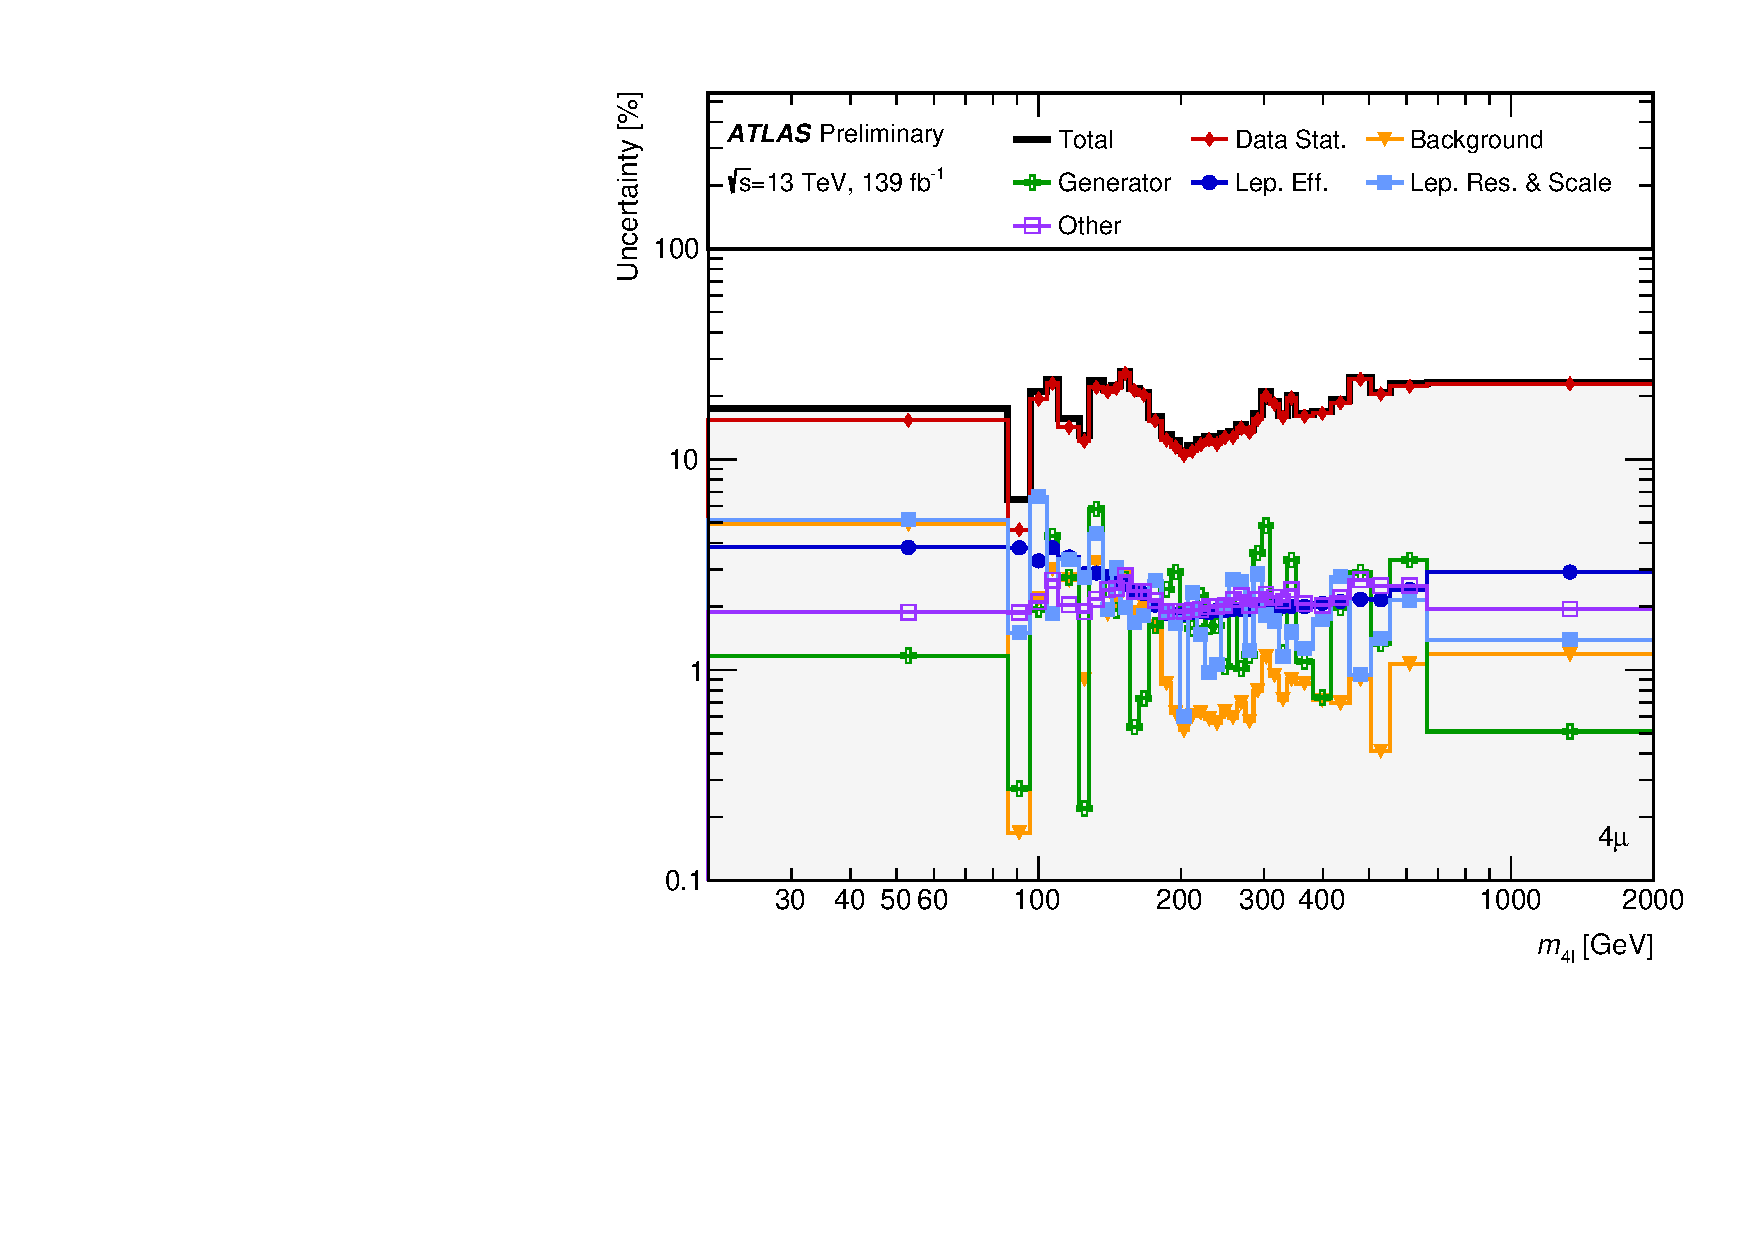
\includegraphics[width = 0.95\textwidth]{Figures/m4l/Systematics/Unfolded/UnfoldedSys_M4lvChannel_Stack_Paper0.pdf}\end{subfigure}
    \begin{subfigure}{.49\textwidth}\centering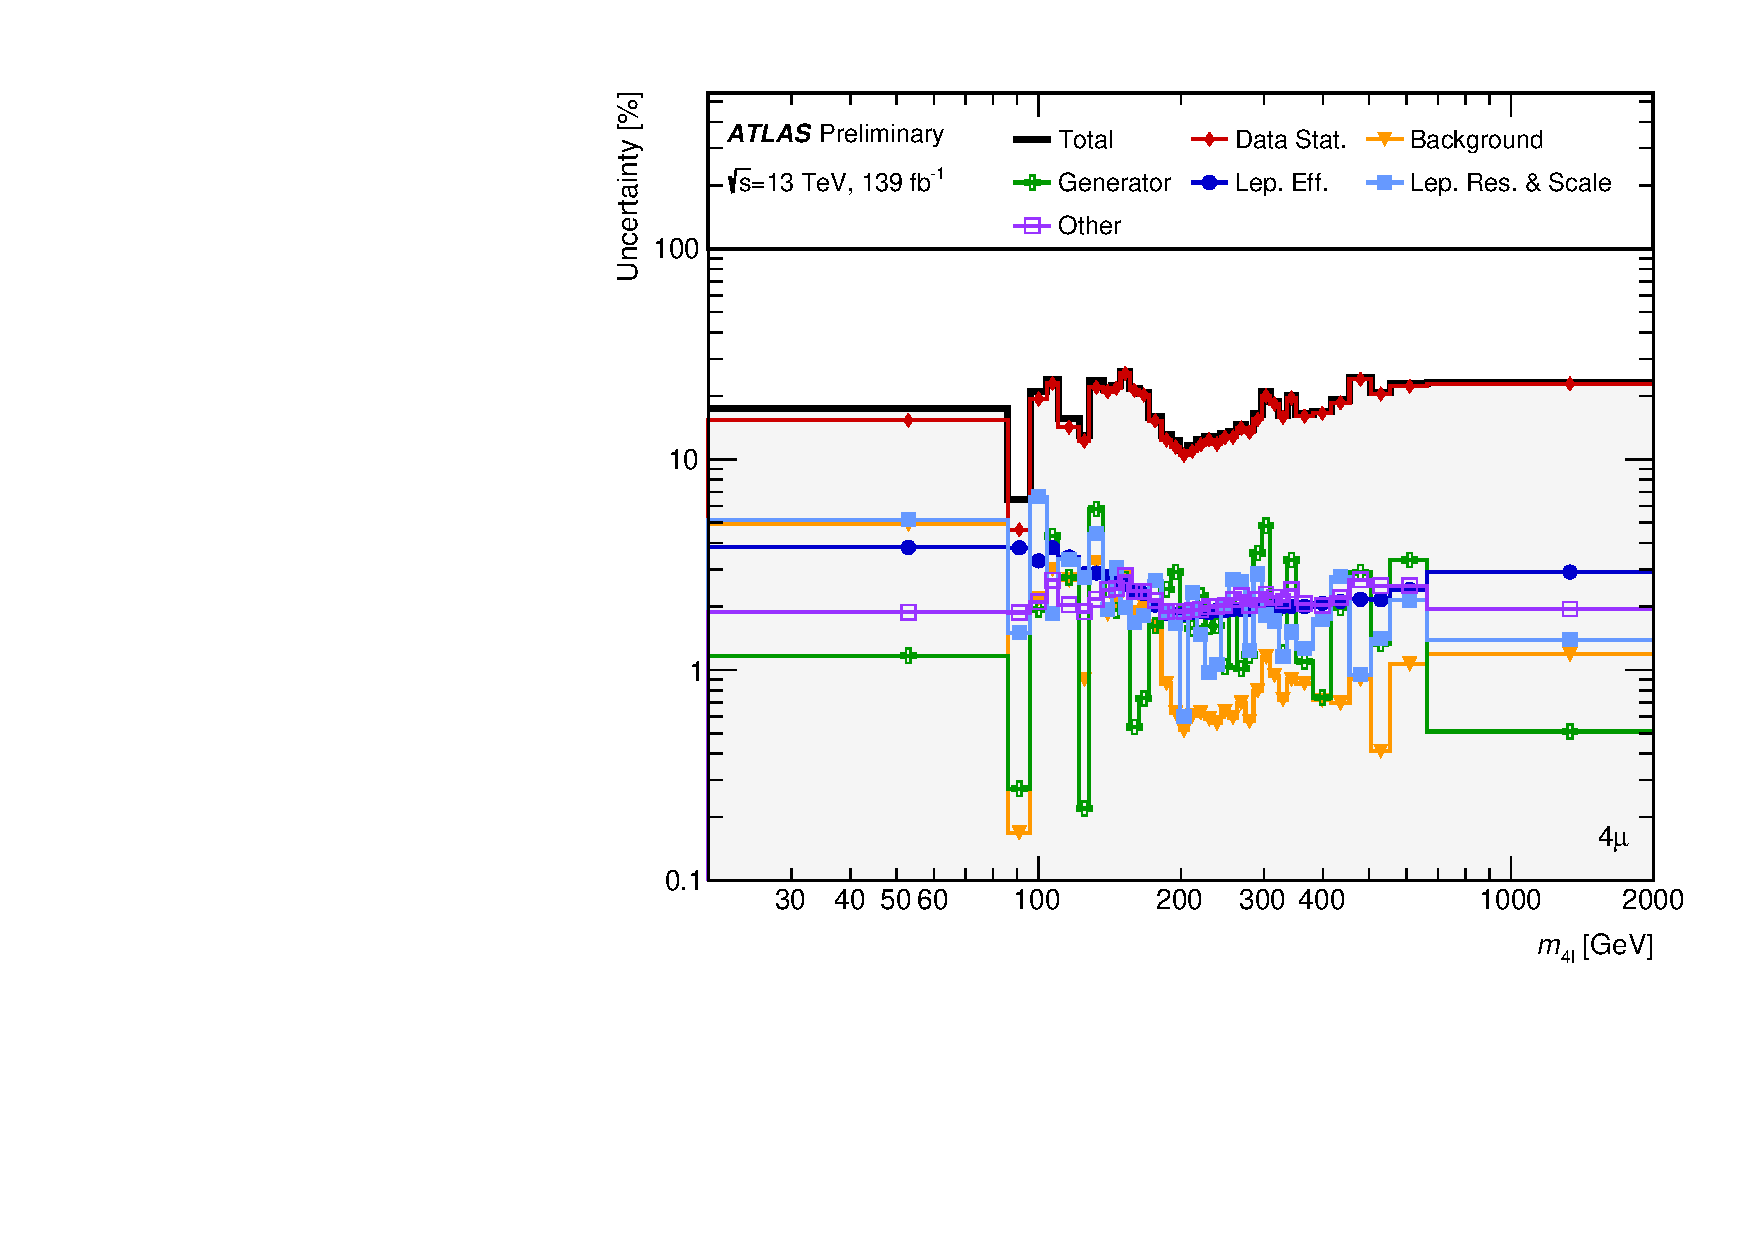
\includegraphics[width = 0.95\textwidth]{Figures/m4l/Systematics/Unfolded/UnfoldedSys_M4lvChannel_Stack_Paper0.pdf}\end{subfigure}
    \begin{subfigure}{.49\textwidth}\centering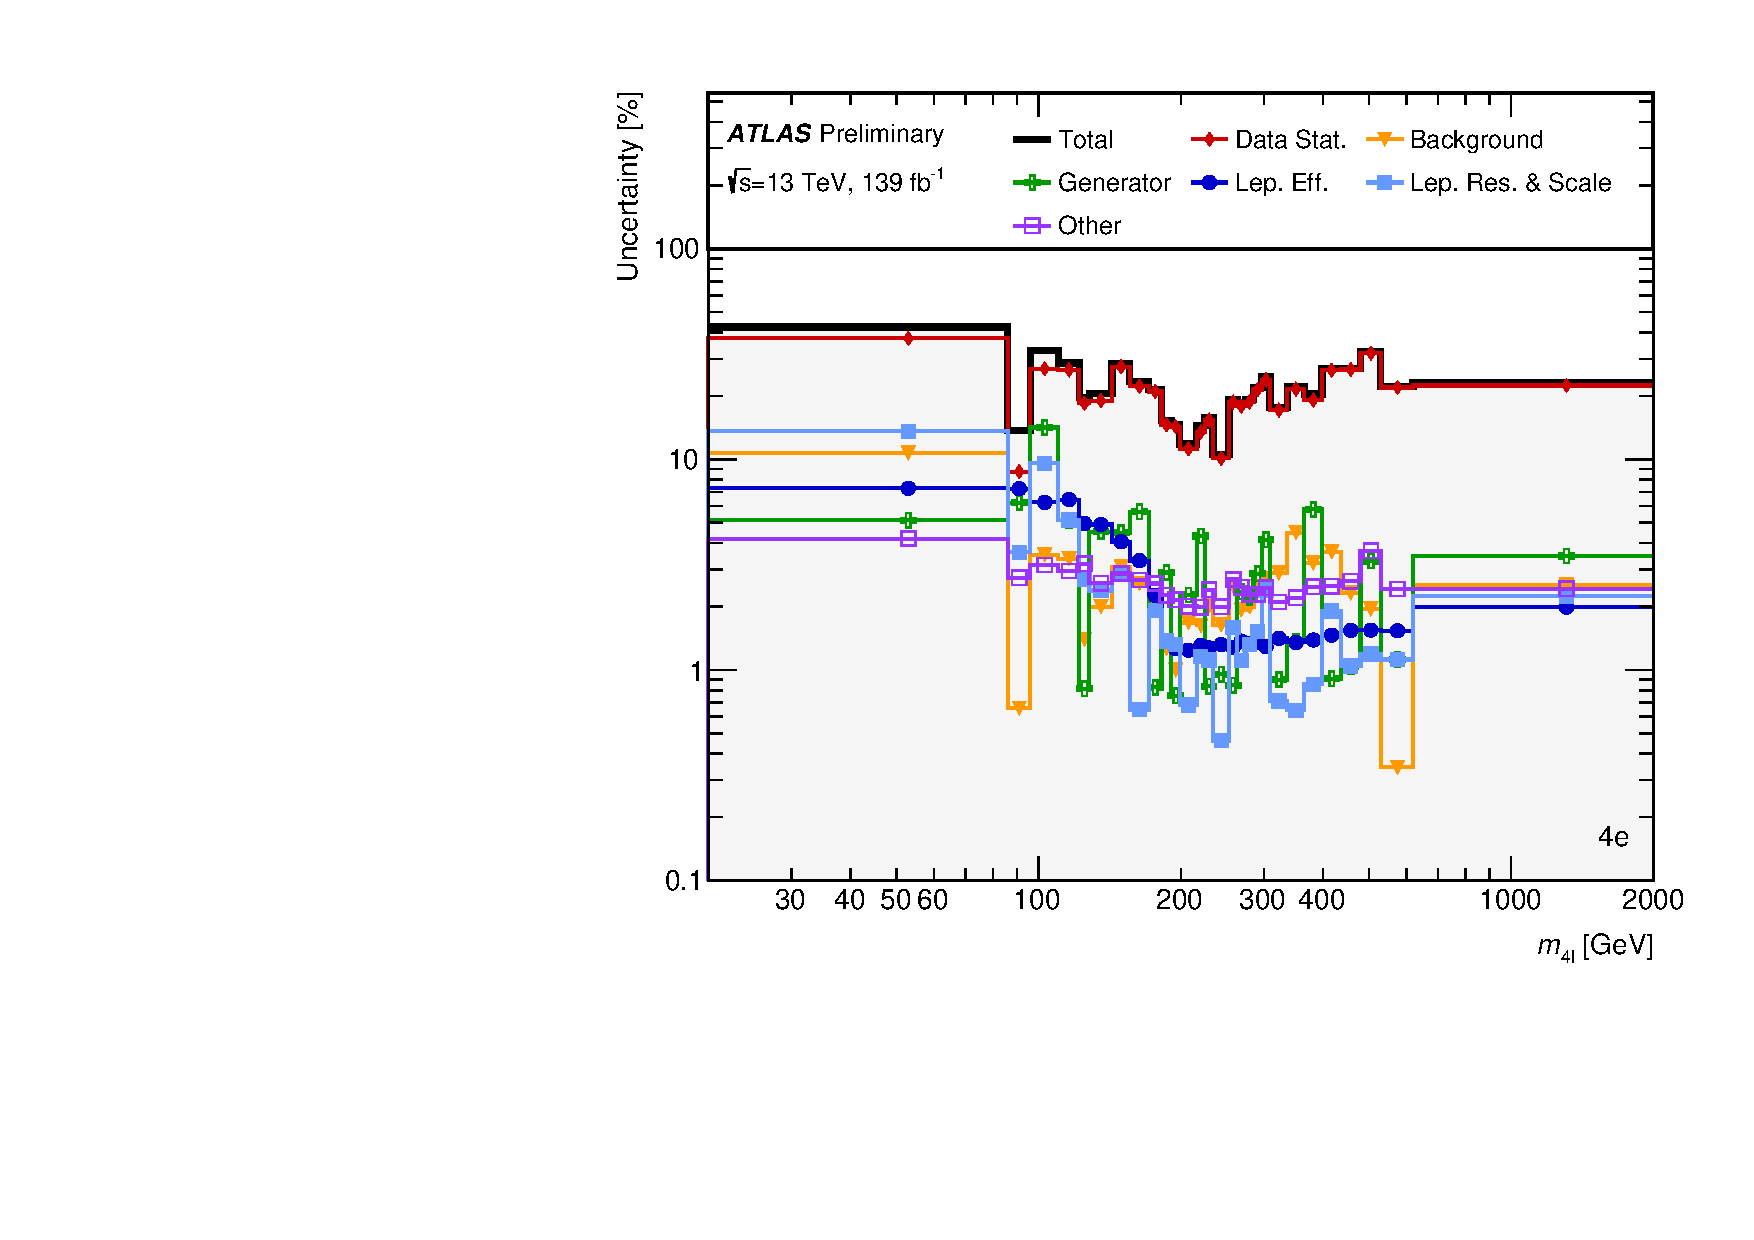
\includegraphics[width = 0.95\textwidth]{Figures/m4l/Systematics/Unfolded/UnfoldedSys_M4lvChannel_Stack_Paper1.pdf}\end{subfigure}
    \begin{subfigure}{.49\textwidth}\centering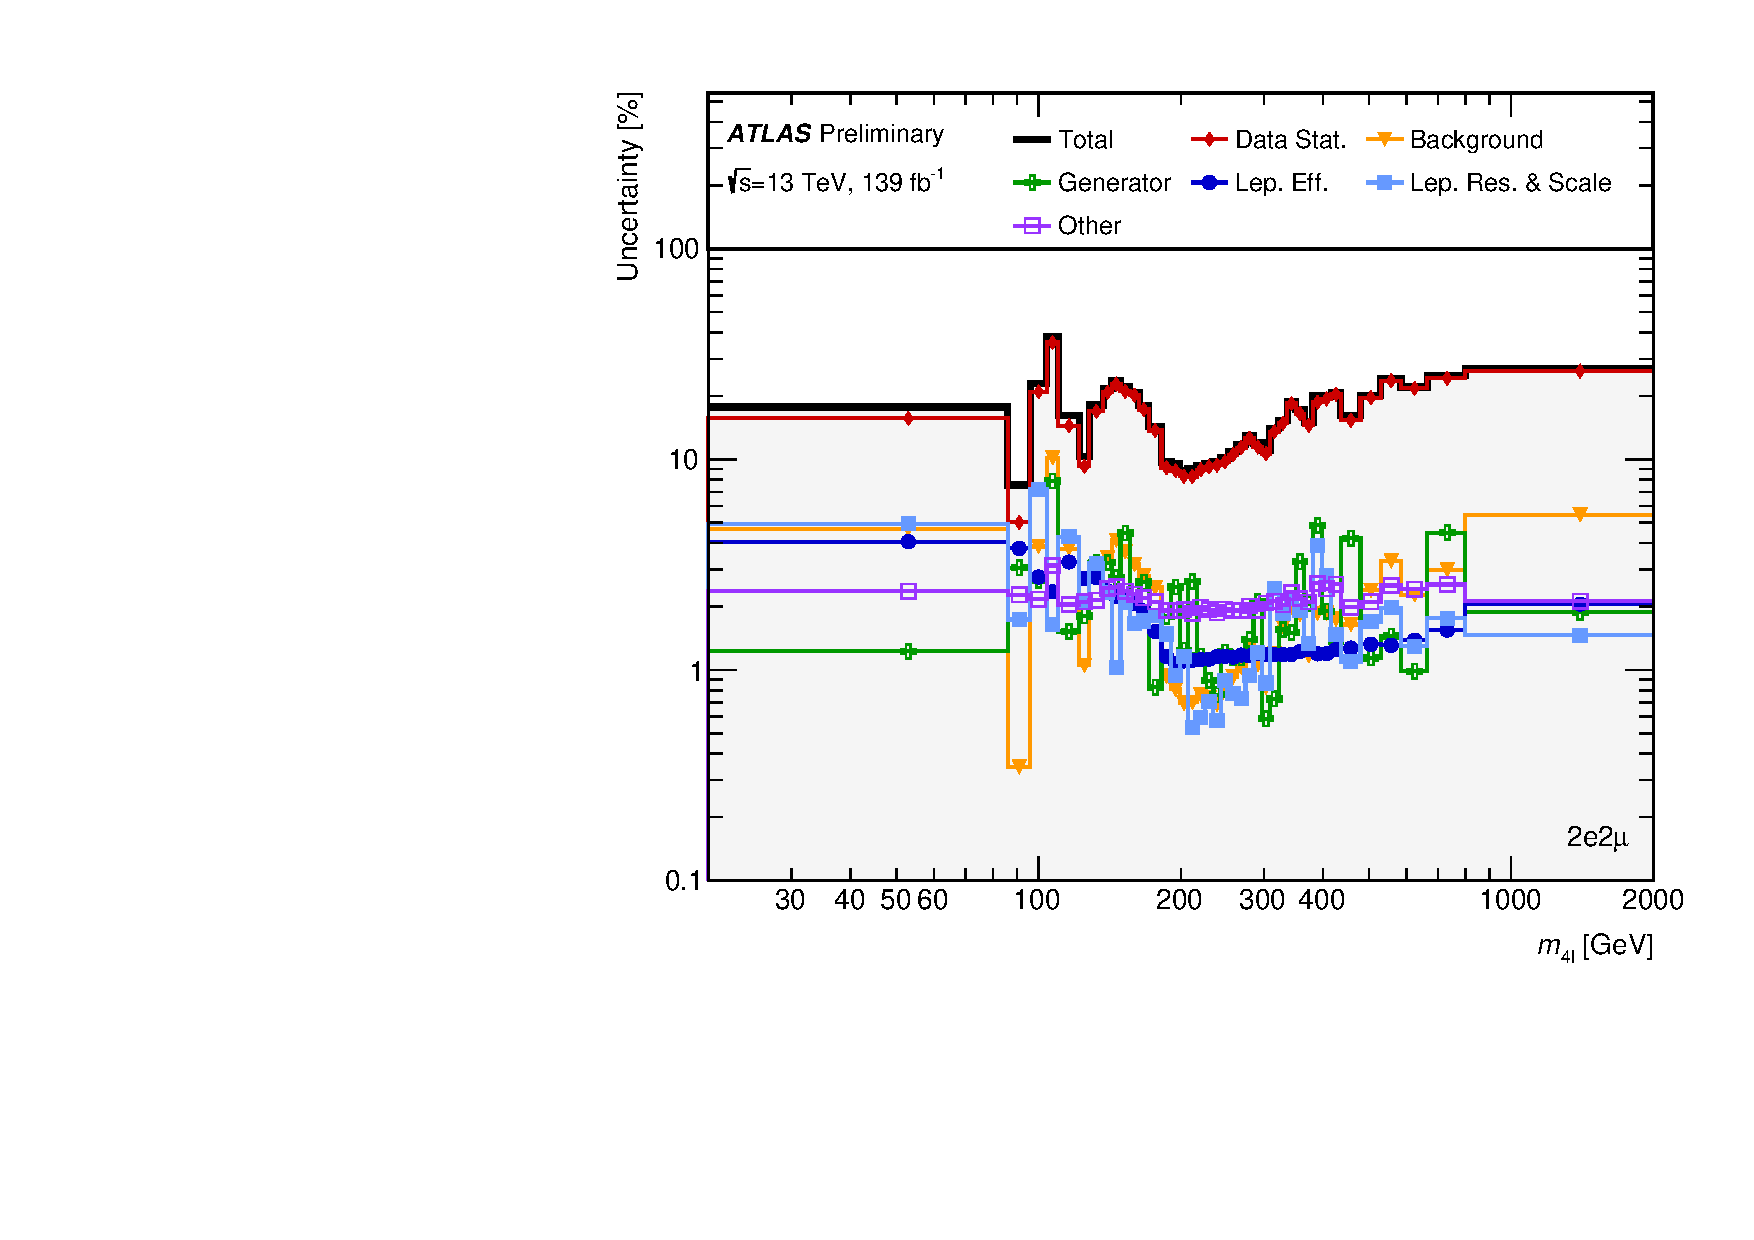
\includegraphics[width = 0.95\textwidth]{Figures/m4l/Systematics/Unfolded/UnfoldedSys_M4lvChannel_Stack_Paper2.pdf}\end{subfigure}
    \caption{Unfolded systematics versus $\mFourL$, in slices of the final-state channel.}
\end{figure}

\begin{figure}[hp]
    \centering
    \begin{subfigure}{.49\textwidth}\centering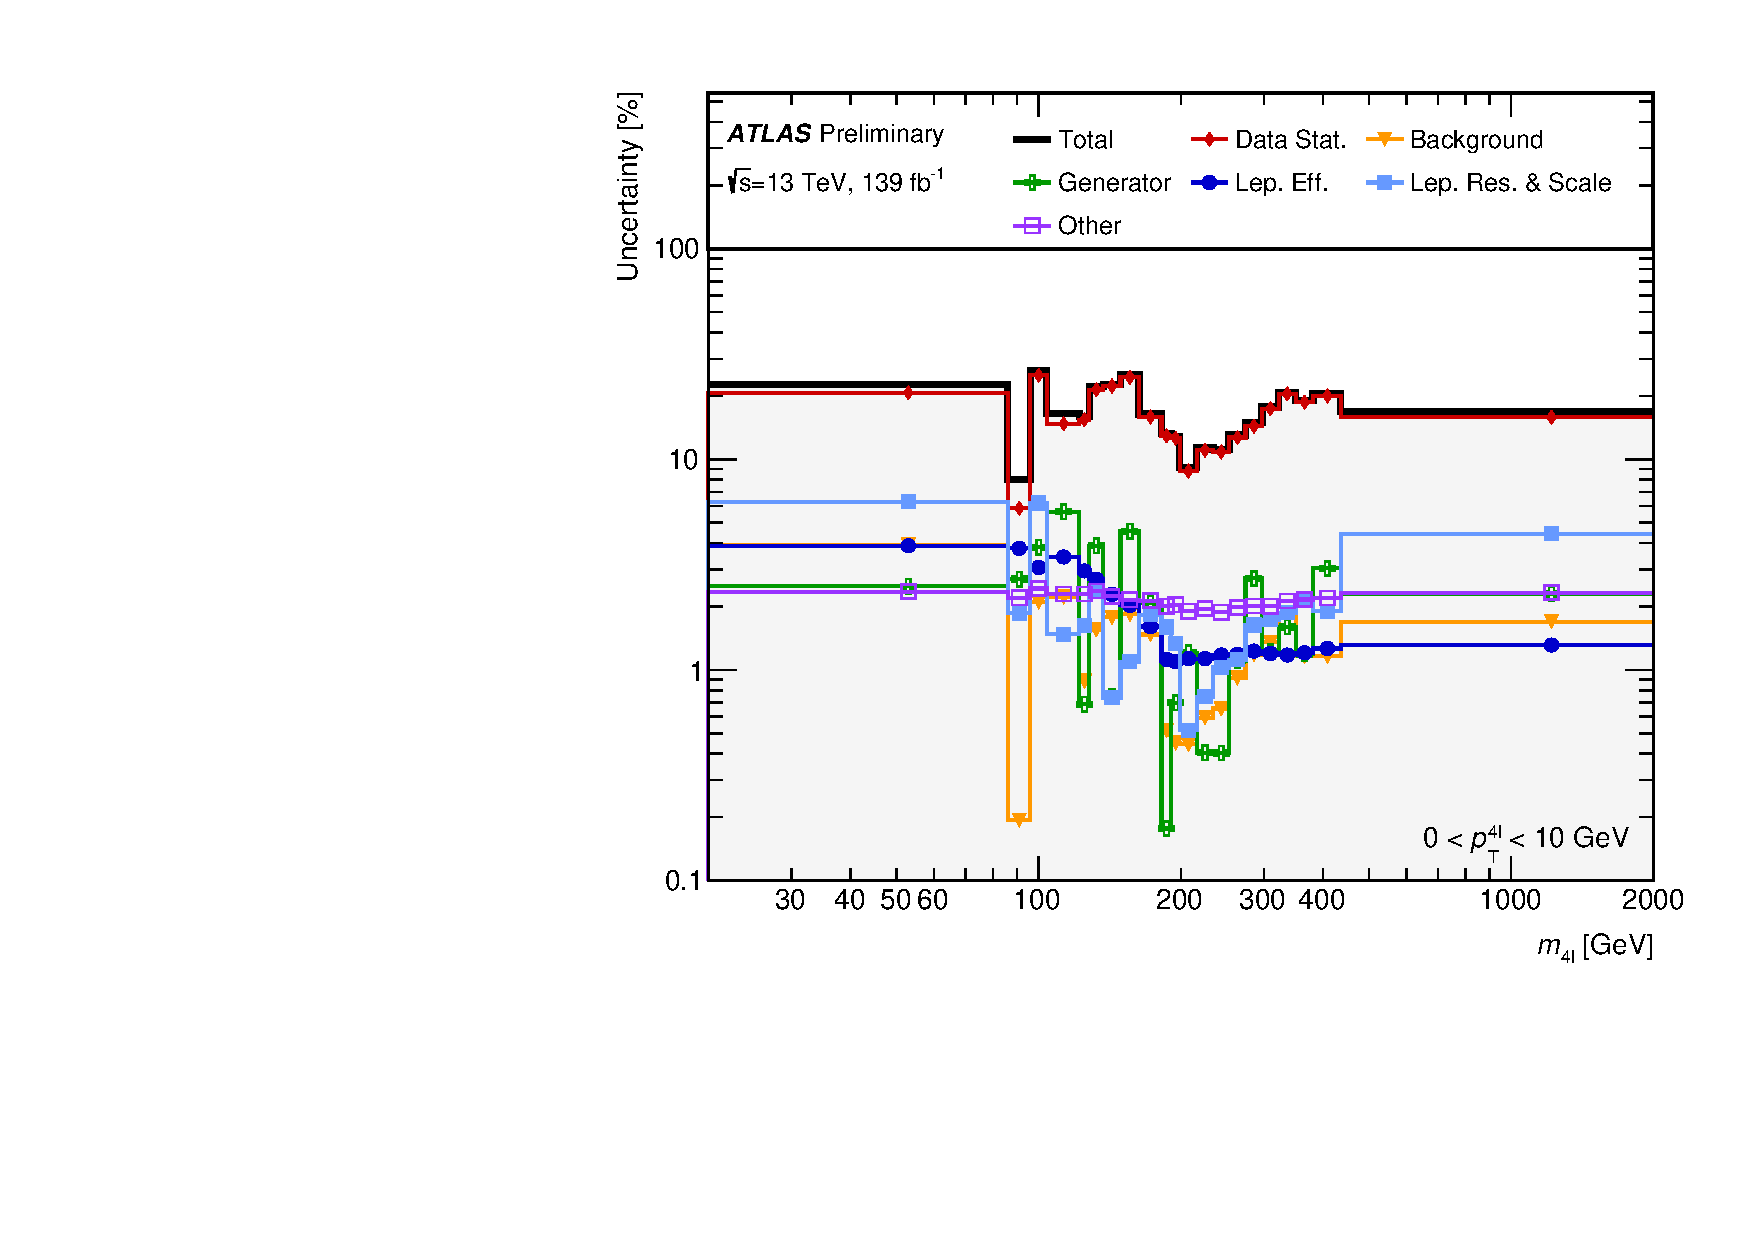
\includegraphics[width = 0.95\textwidth]{Figures/m4l/Systematics/Unfolded/UnfoldedSys_M4lvPt4lbin_Stack_Paper0.pdf}\end{subfigure}
    \begin{subfigure}{.49\textwidth}\centering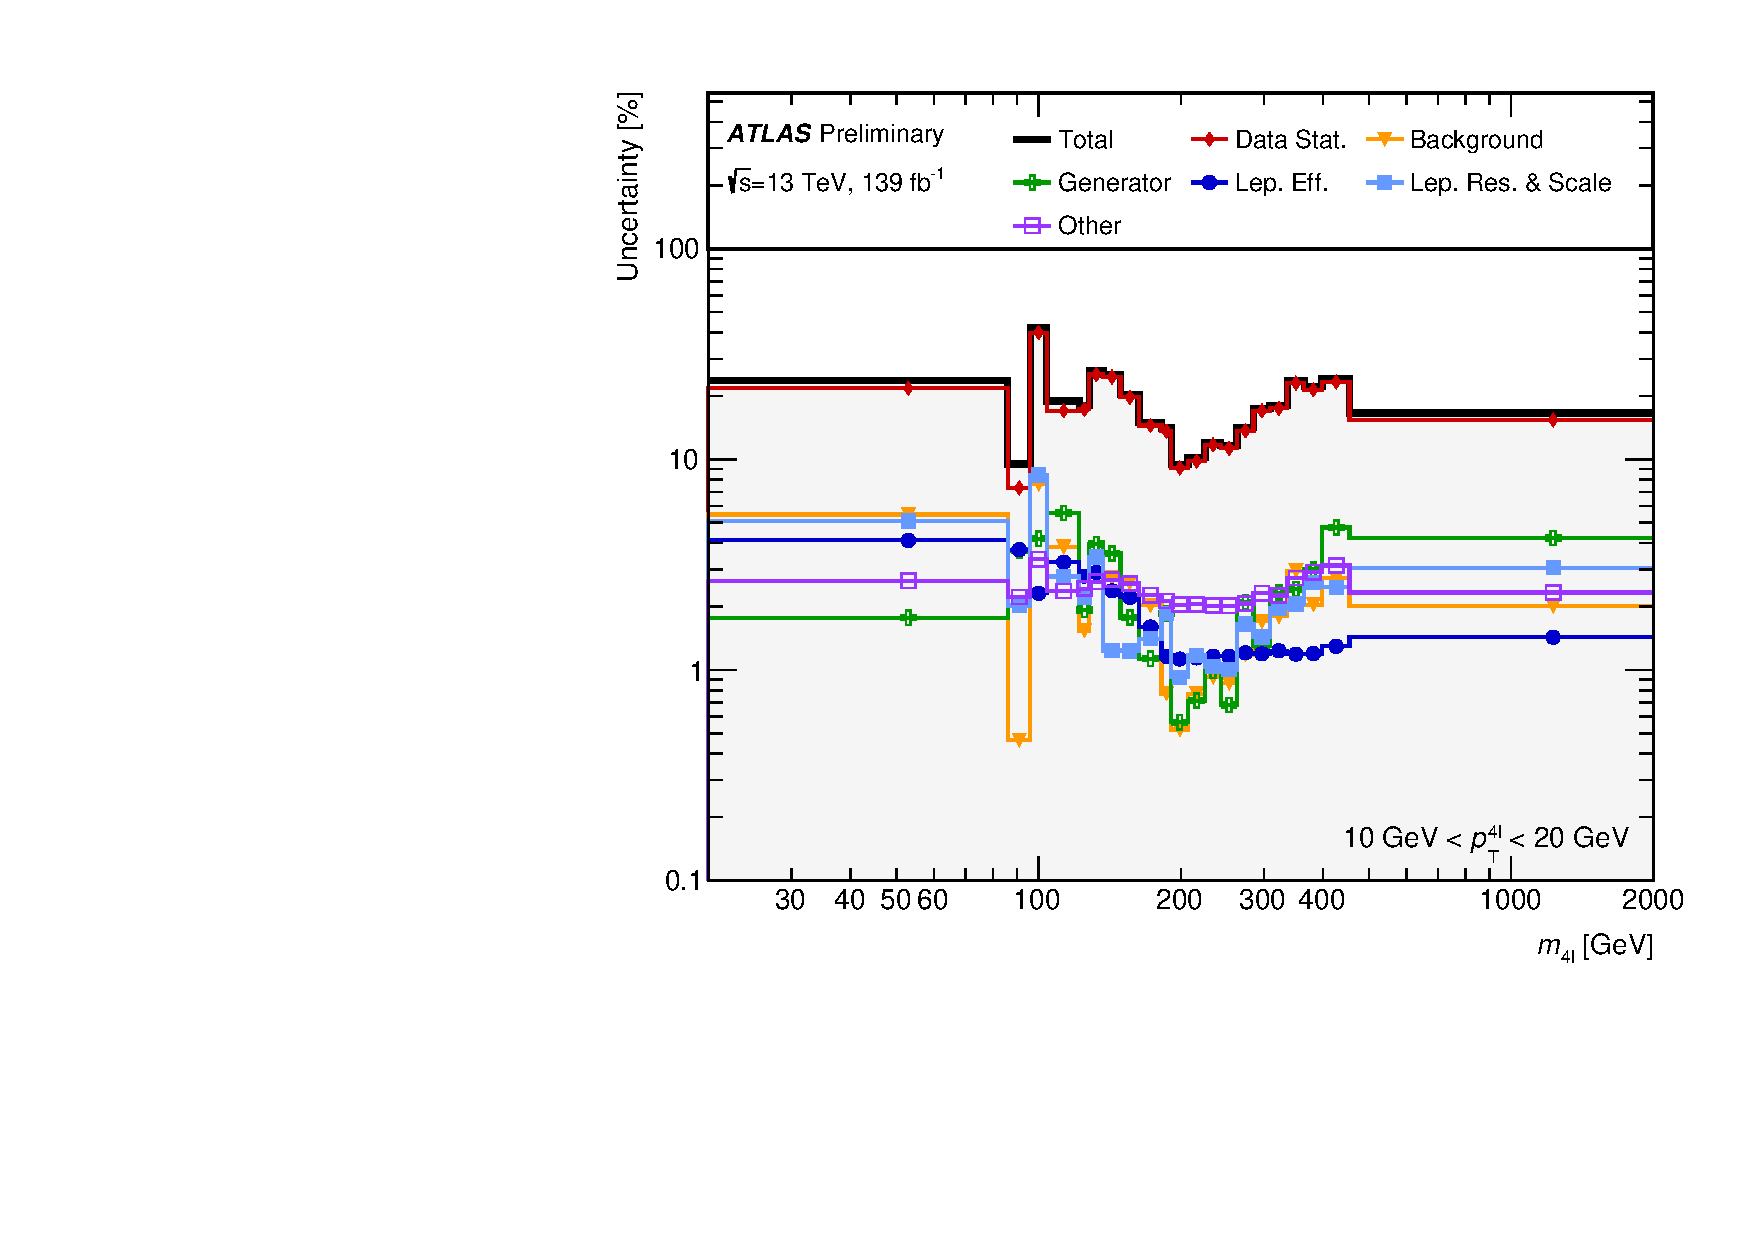
\includegraphics[width = 0.95\textwidth]{Figures/m4l/Systematics/Unfolded/UnfoldedSys_M4lvPt4lbin_Stack_Paper1.pdf}\end{subfigure}
    \begin{subfigure}{.49\textwidth}\centering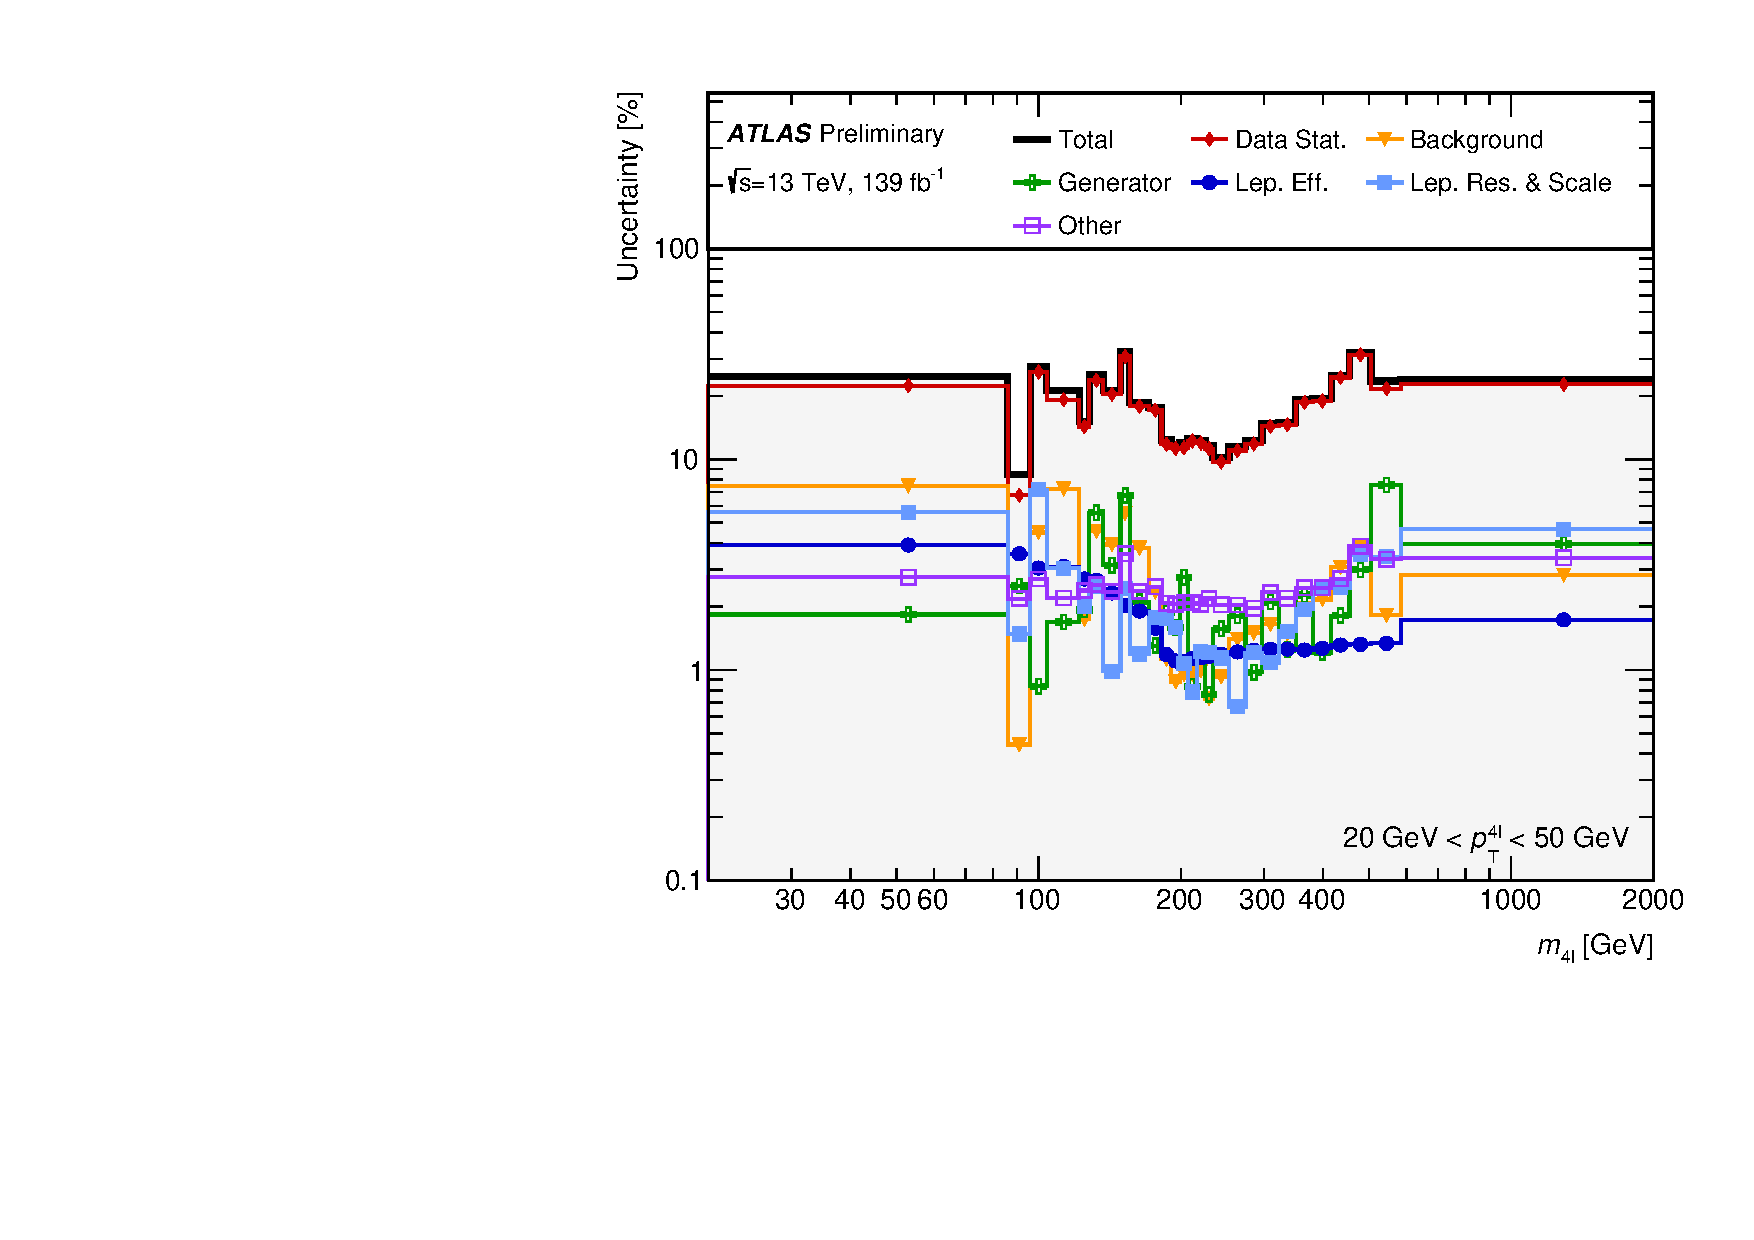
\includegraphics[width = 0.95\textwidth]{Figures/m4l/Systematics/Unfolded/UnfoldedSys_M4lvPt4lbin_Stack_Paper2.pdf}\end{subfigure}
    \begin{subfigure}{.49\textwidth}\centering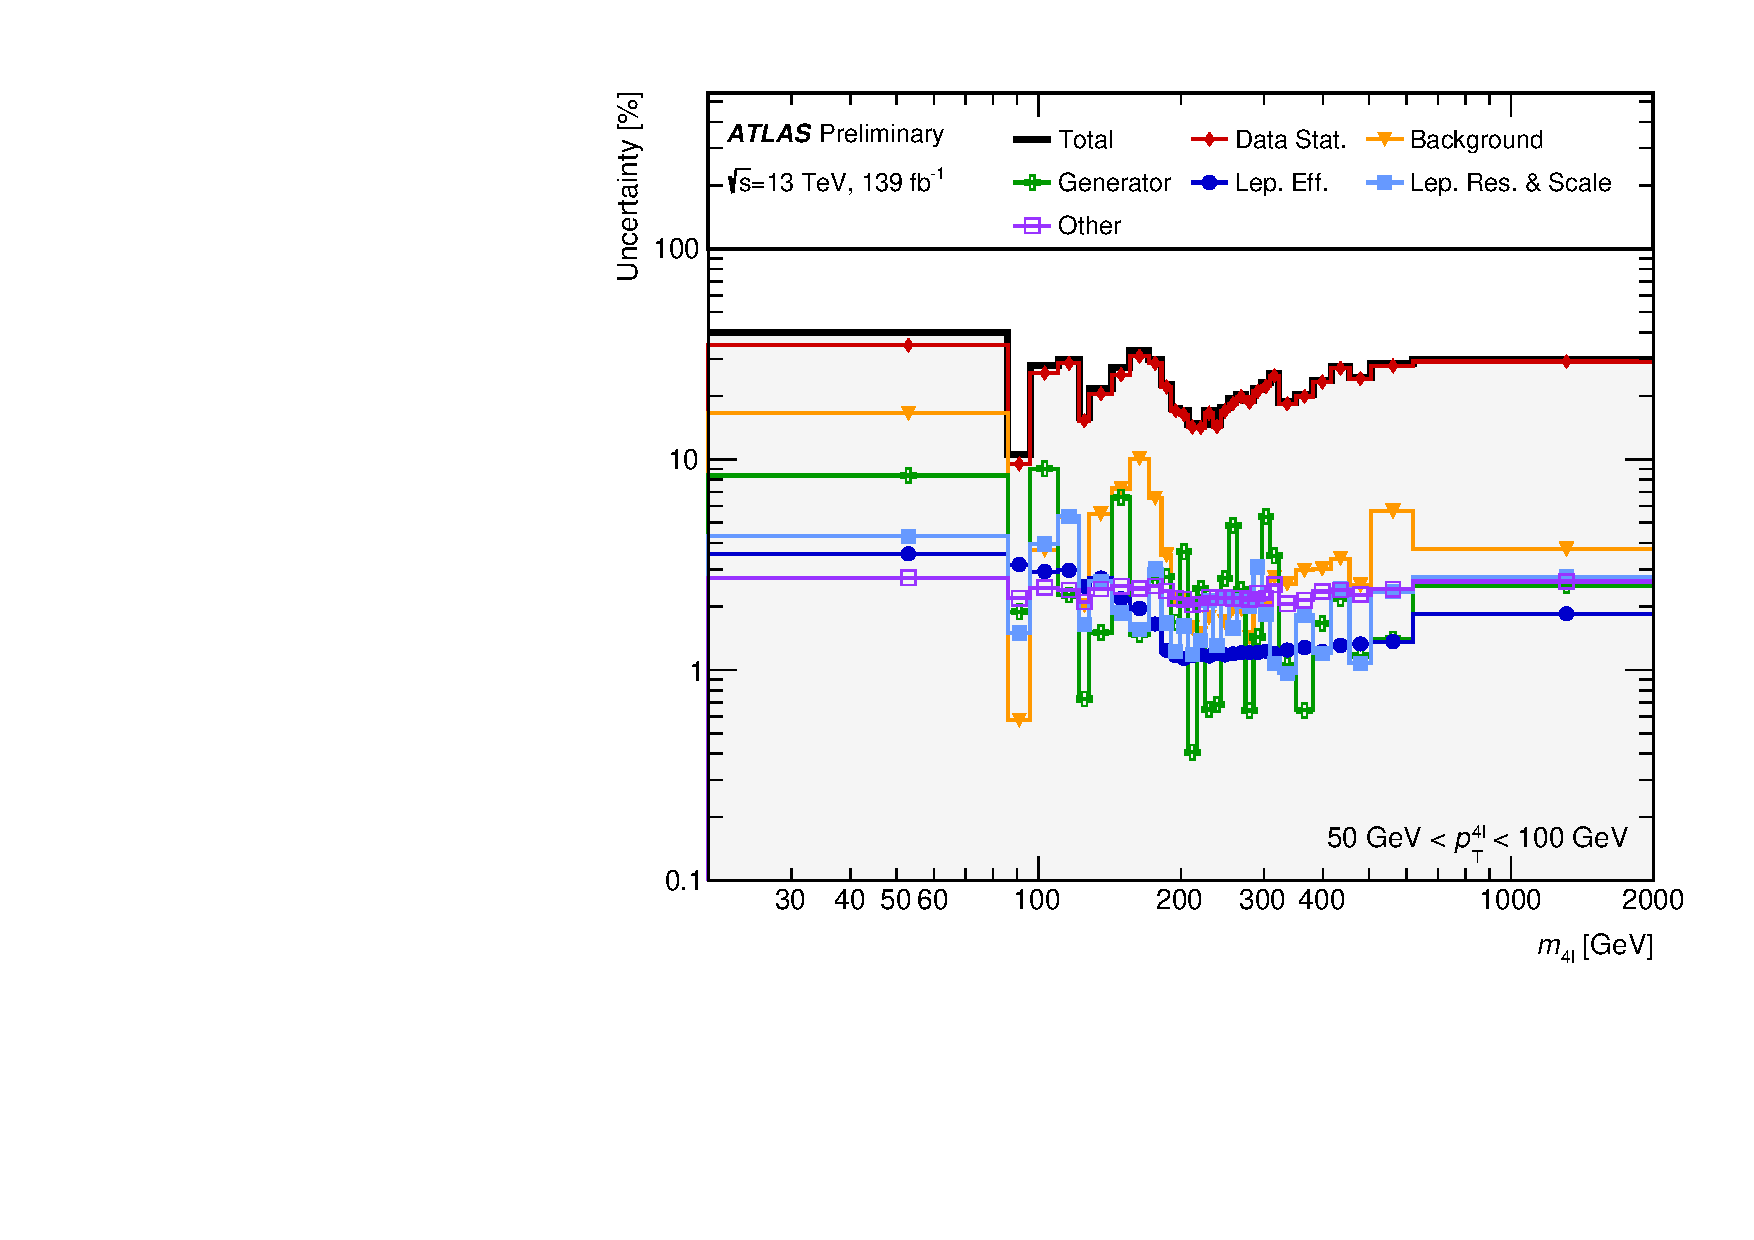
\includegraphics[width = 0.95\textwidth]{Figures/m4l/Systematics/Unfolded/UnfoldedSys_M4lvPt4lbin_Stack_Paper3.pdf}\end{subfigure}
    \begin{subfigure}{.49\textwidth}\centering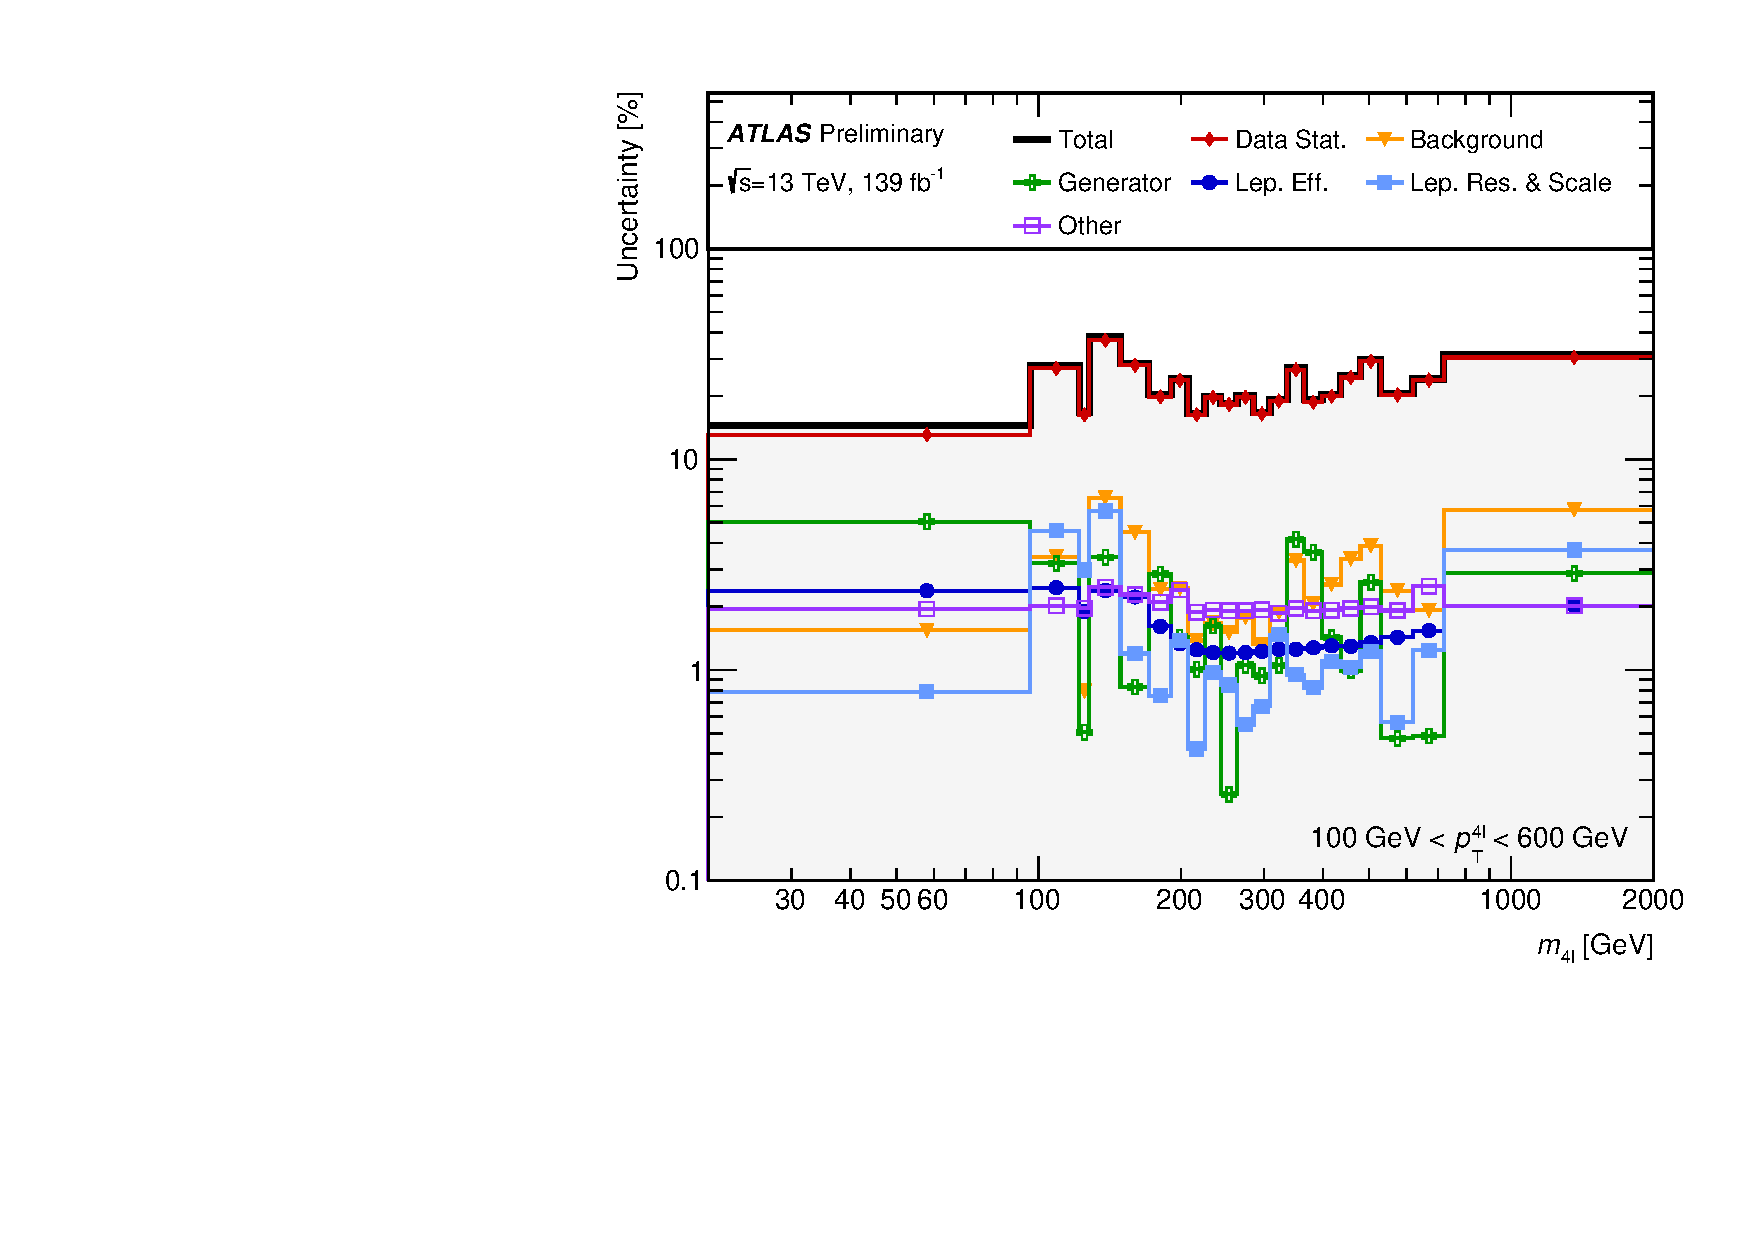
\includegraphics[width = 0.95\textwidth]{Figures/m4l/Systematics/Unfolded/UnfoldedSys_M4lvPt4lbin_Stack_Paper4.pdf}\end{subfigure}
    \caption{Unfolded systematics versus $\mFourL$, in slices of $\ptFourL$.}
\end{figure}

\begin{figure}[hp]
    \centering
    \begin{subfigure}{.49\textwidth}\centering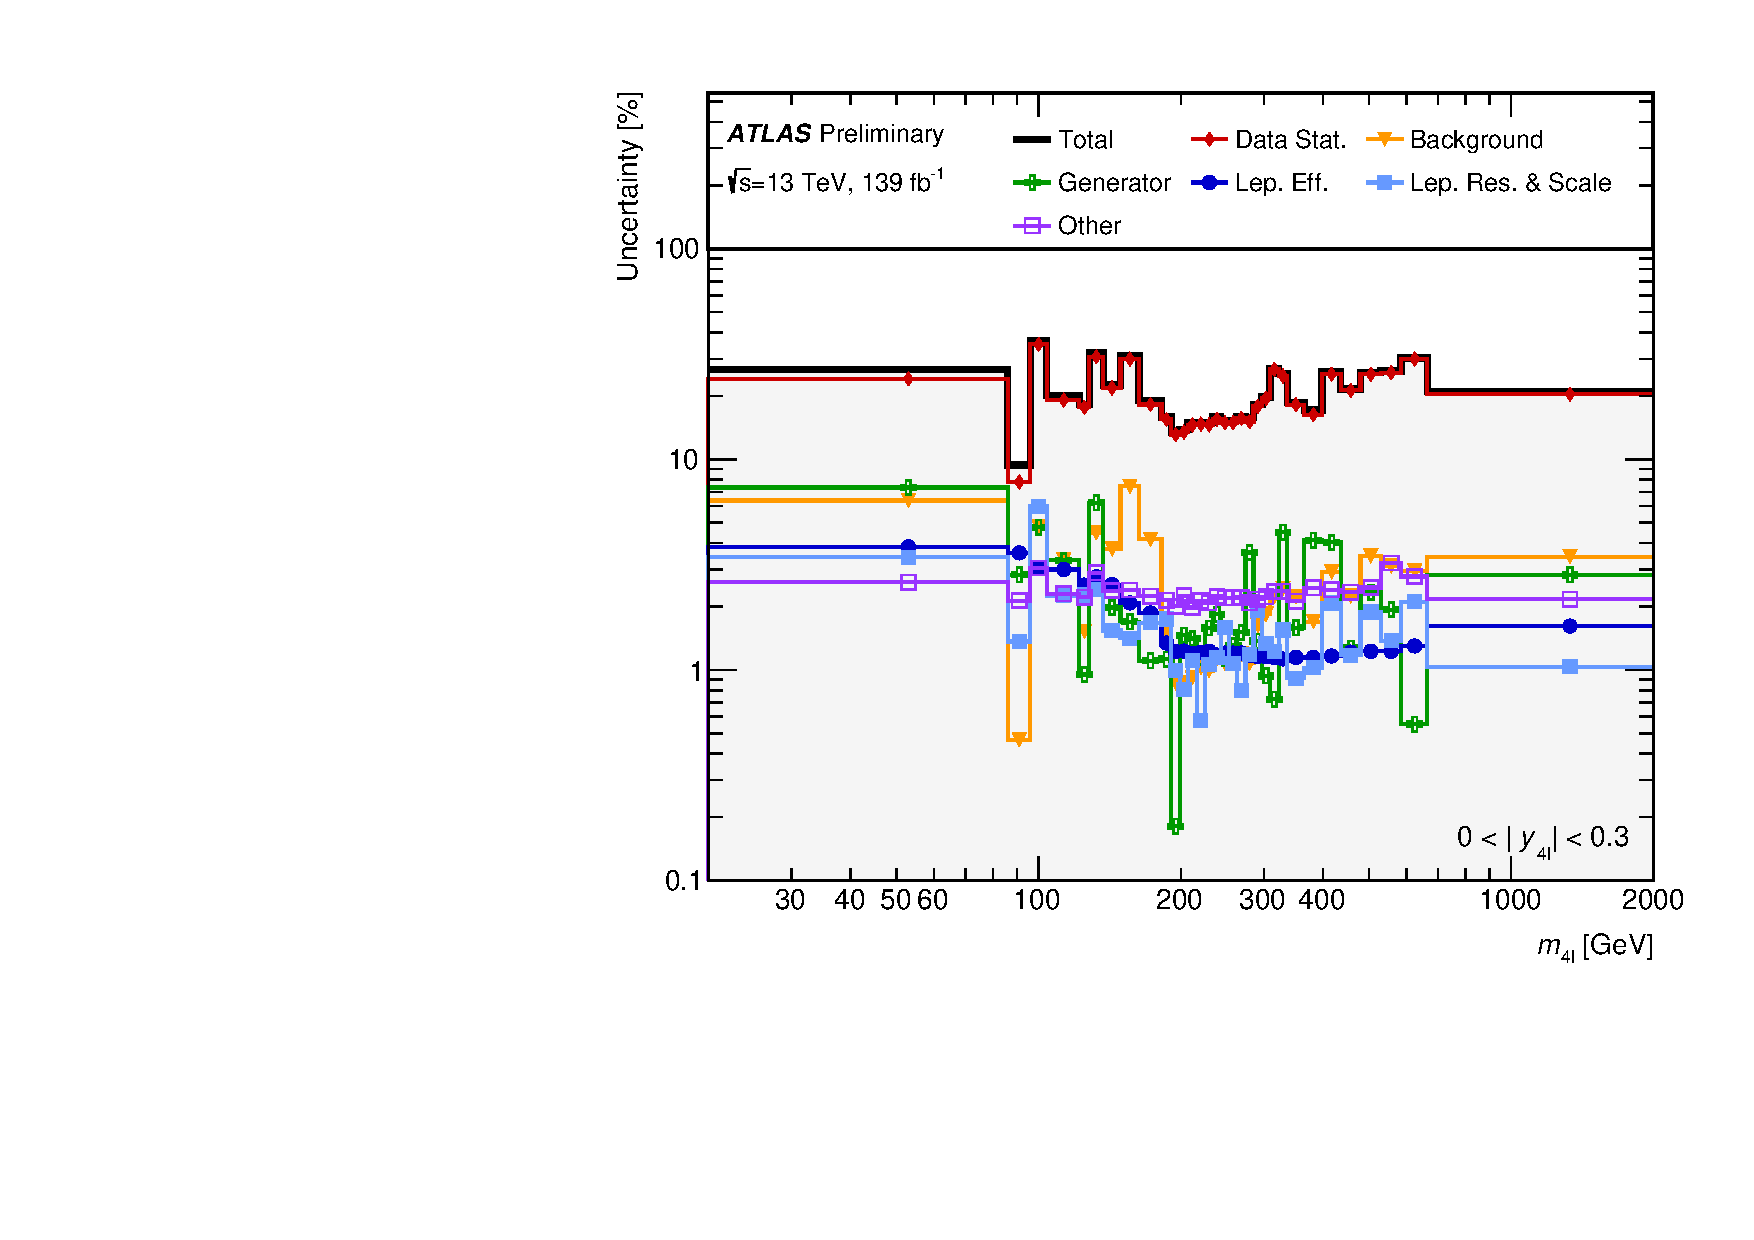
\includegraphics[width = 0.95\textwidth]{Figures/m4l/Systematics/Unfolded/UnfoldedSys_M4lvRapiditybin_Stack_Paper0.pdf}\end{subfigure}
    \begin{subfigure}{.49\textwidth}\centering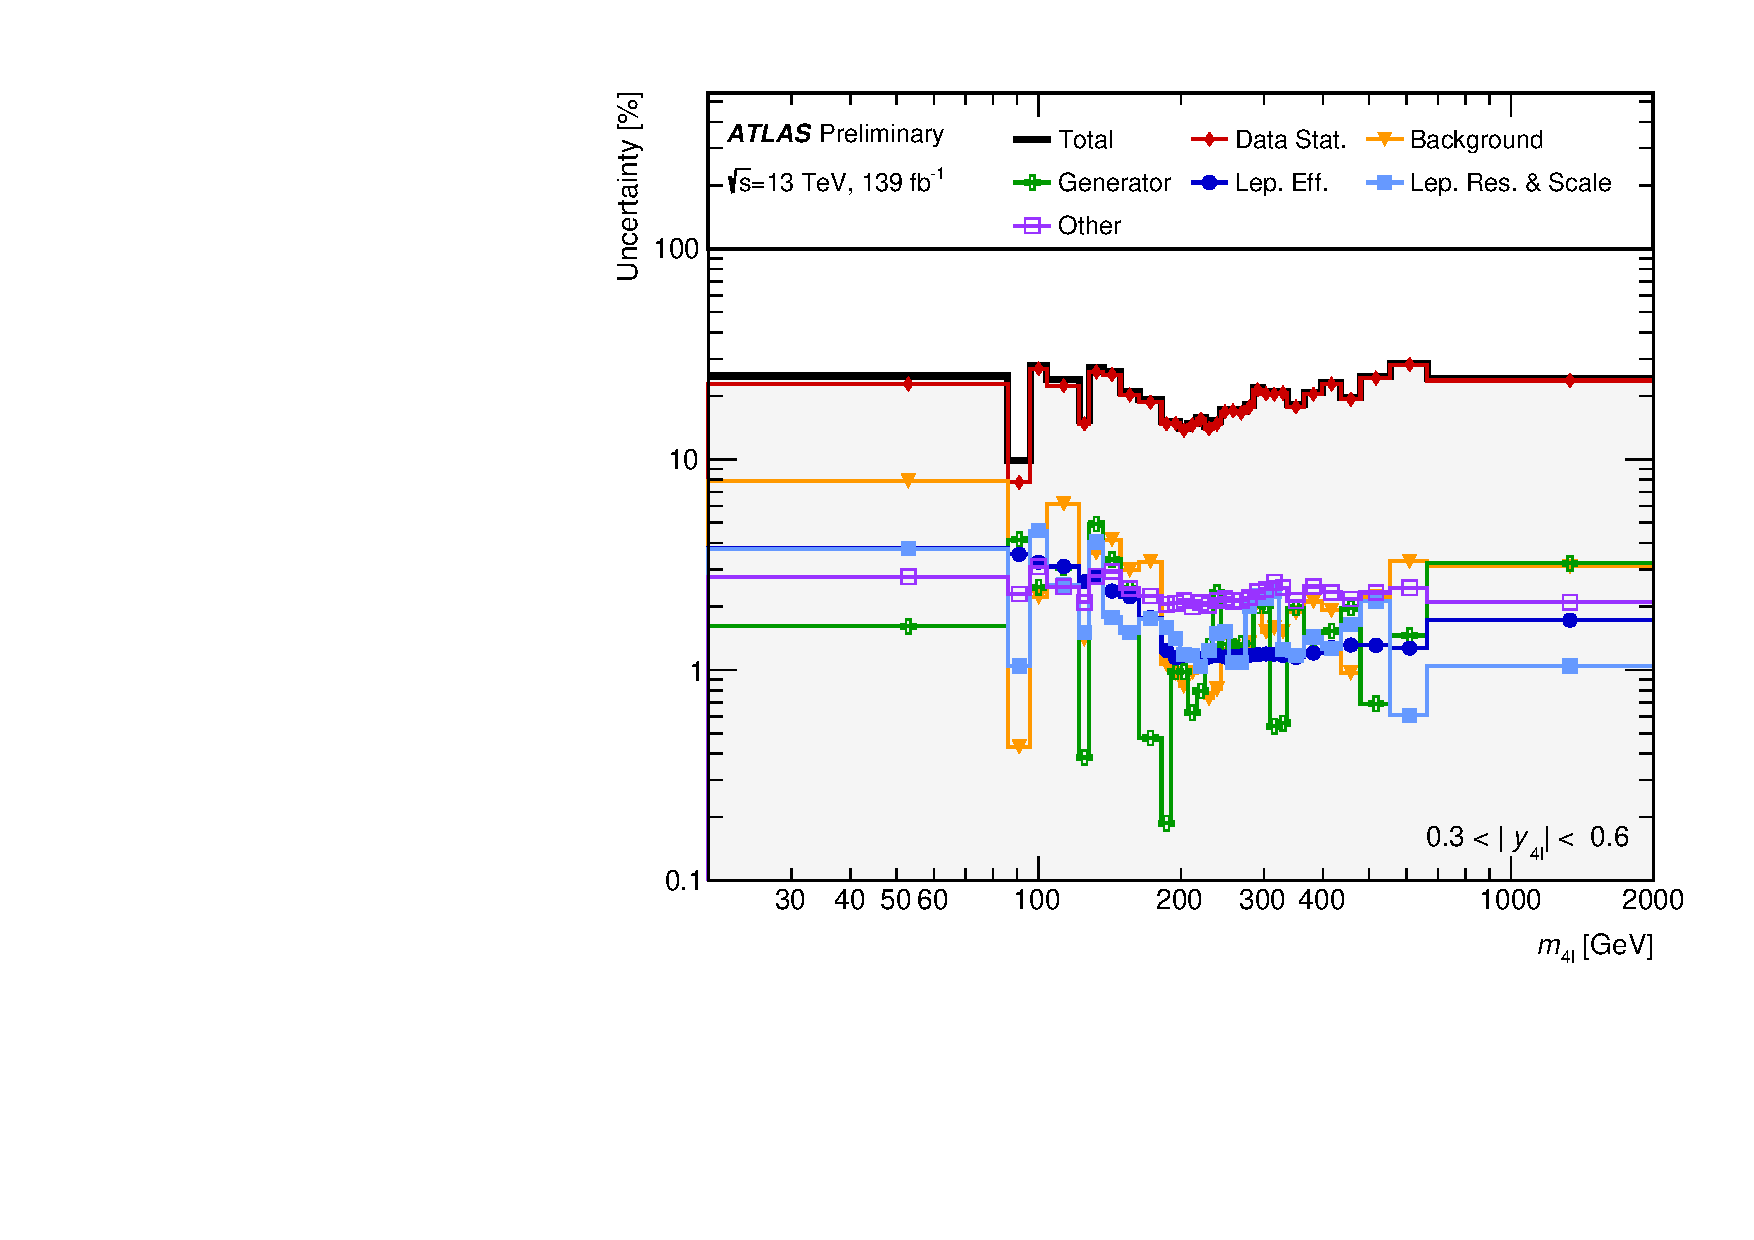
\includegraphics[width = 0.95\textwidth]{Figures/m4l/Systematics/Unfolded/UnfoldedSys_M4lvRapiditybin_Stack_Paper1.pdf}\end{subfigure}
    \begin{subfigure}{.49\textwidth}\centering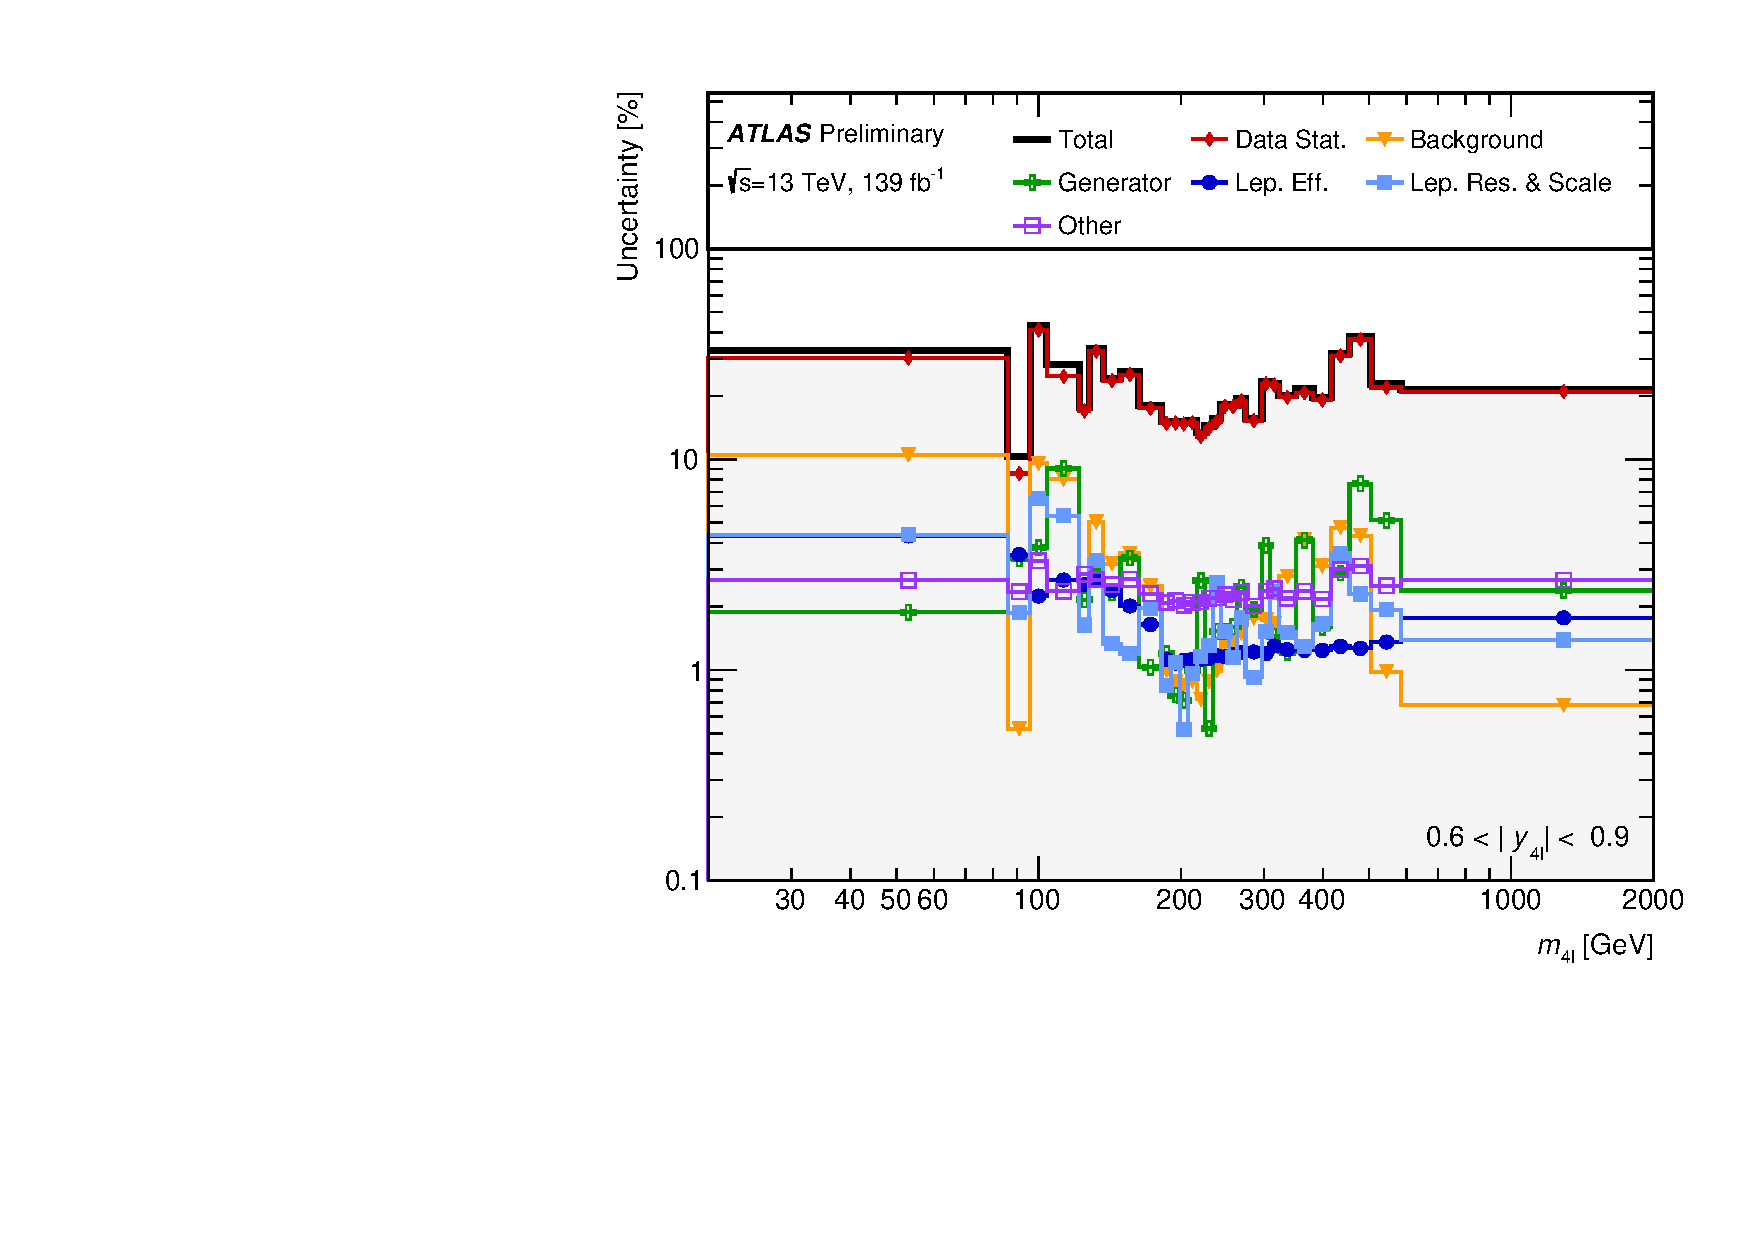
\includegraphics[width = 0.95\textwidth]{Figures/m4l/Systematics/Unfolded/UnfoldedSys_M4lvRapiditybin_Stack_Paper2.pdf}\end{subfigure}
    \begin{subfigure}{.49\textwidth}\centering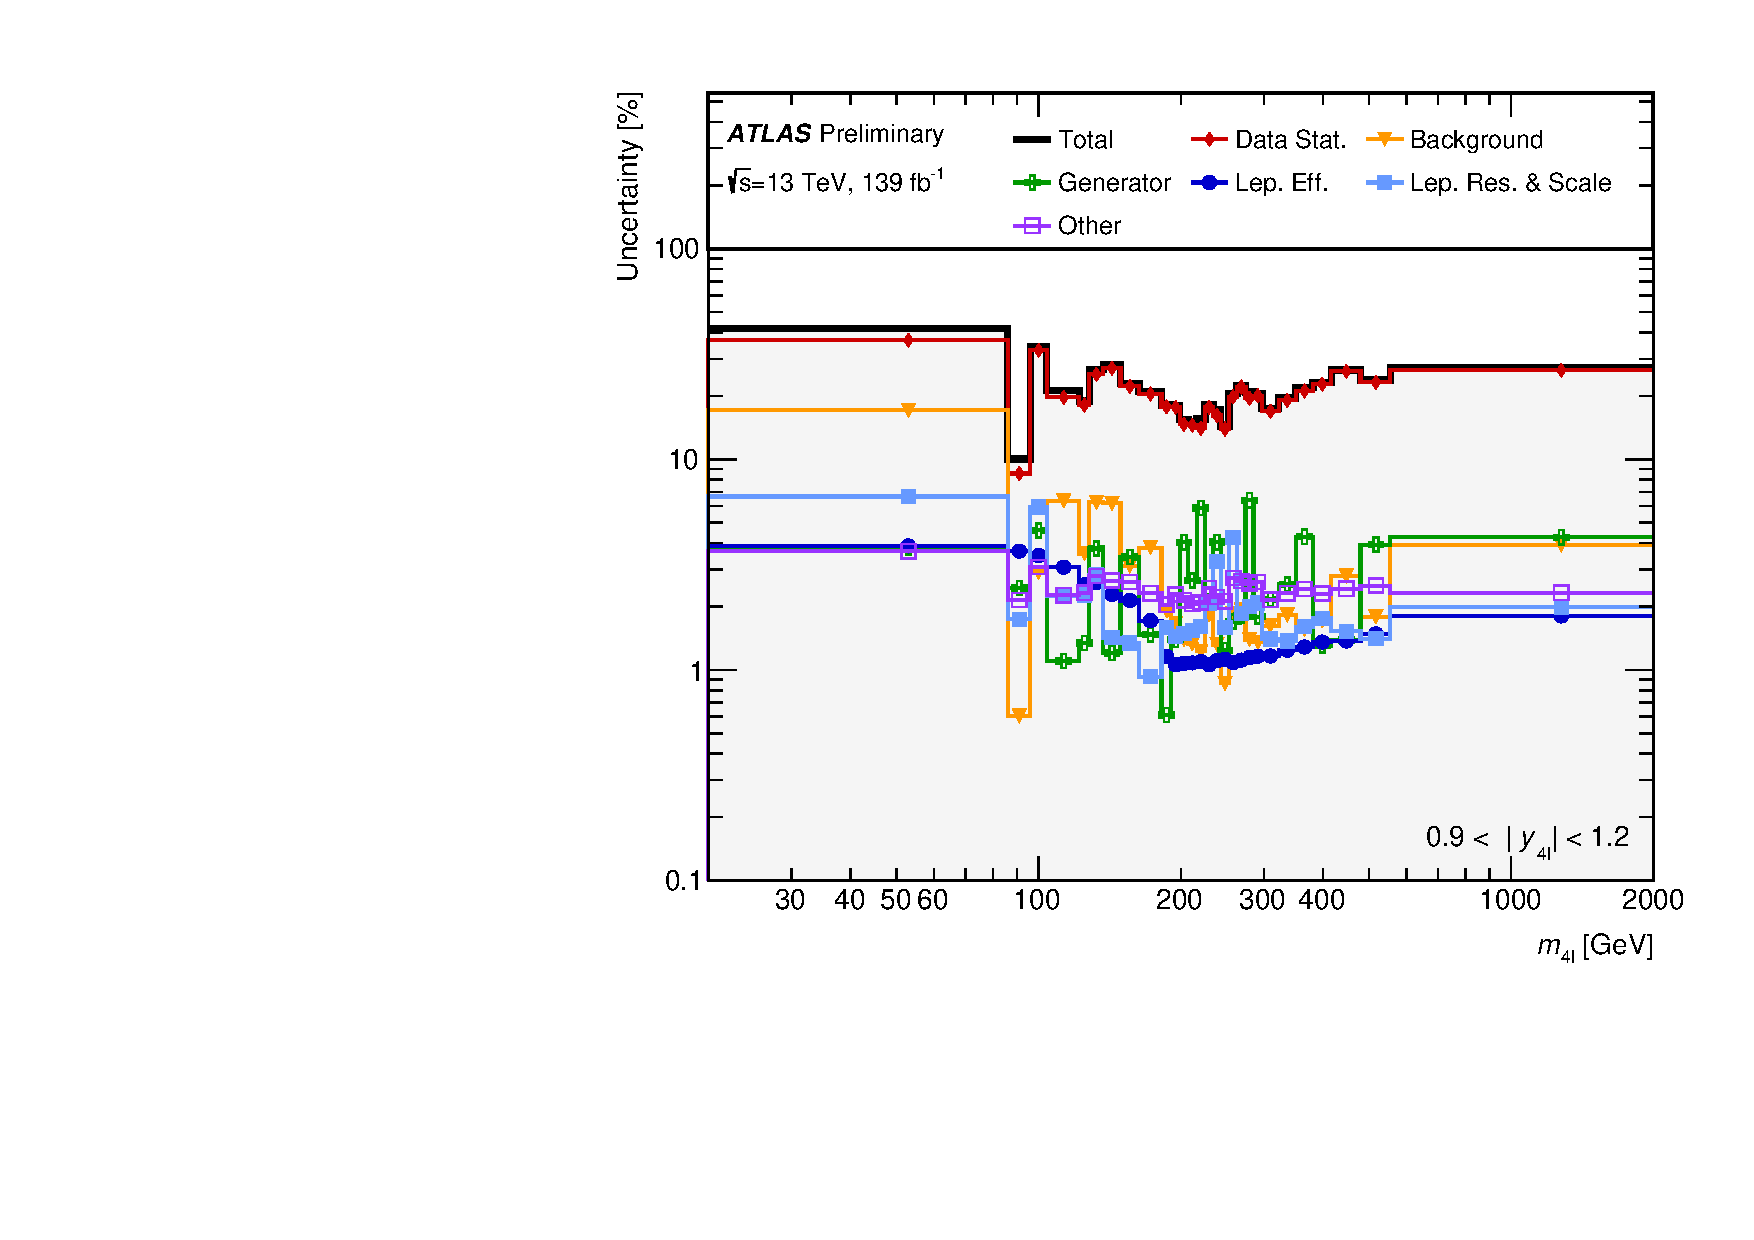
\includegraphics[width = 0.95\textwidth]{Figures/m4l/Systematics/Unfolded/UnfoldedSys_M4lvRapiditybin_Stack_Paper3.pdf}\end{subfigure}
    \begin{subfigure}{.49\textwidth}\centering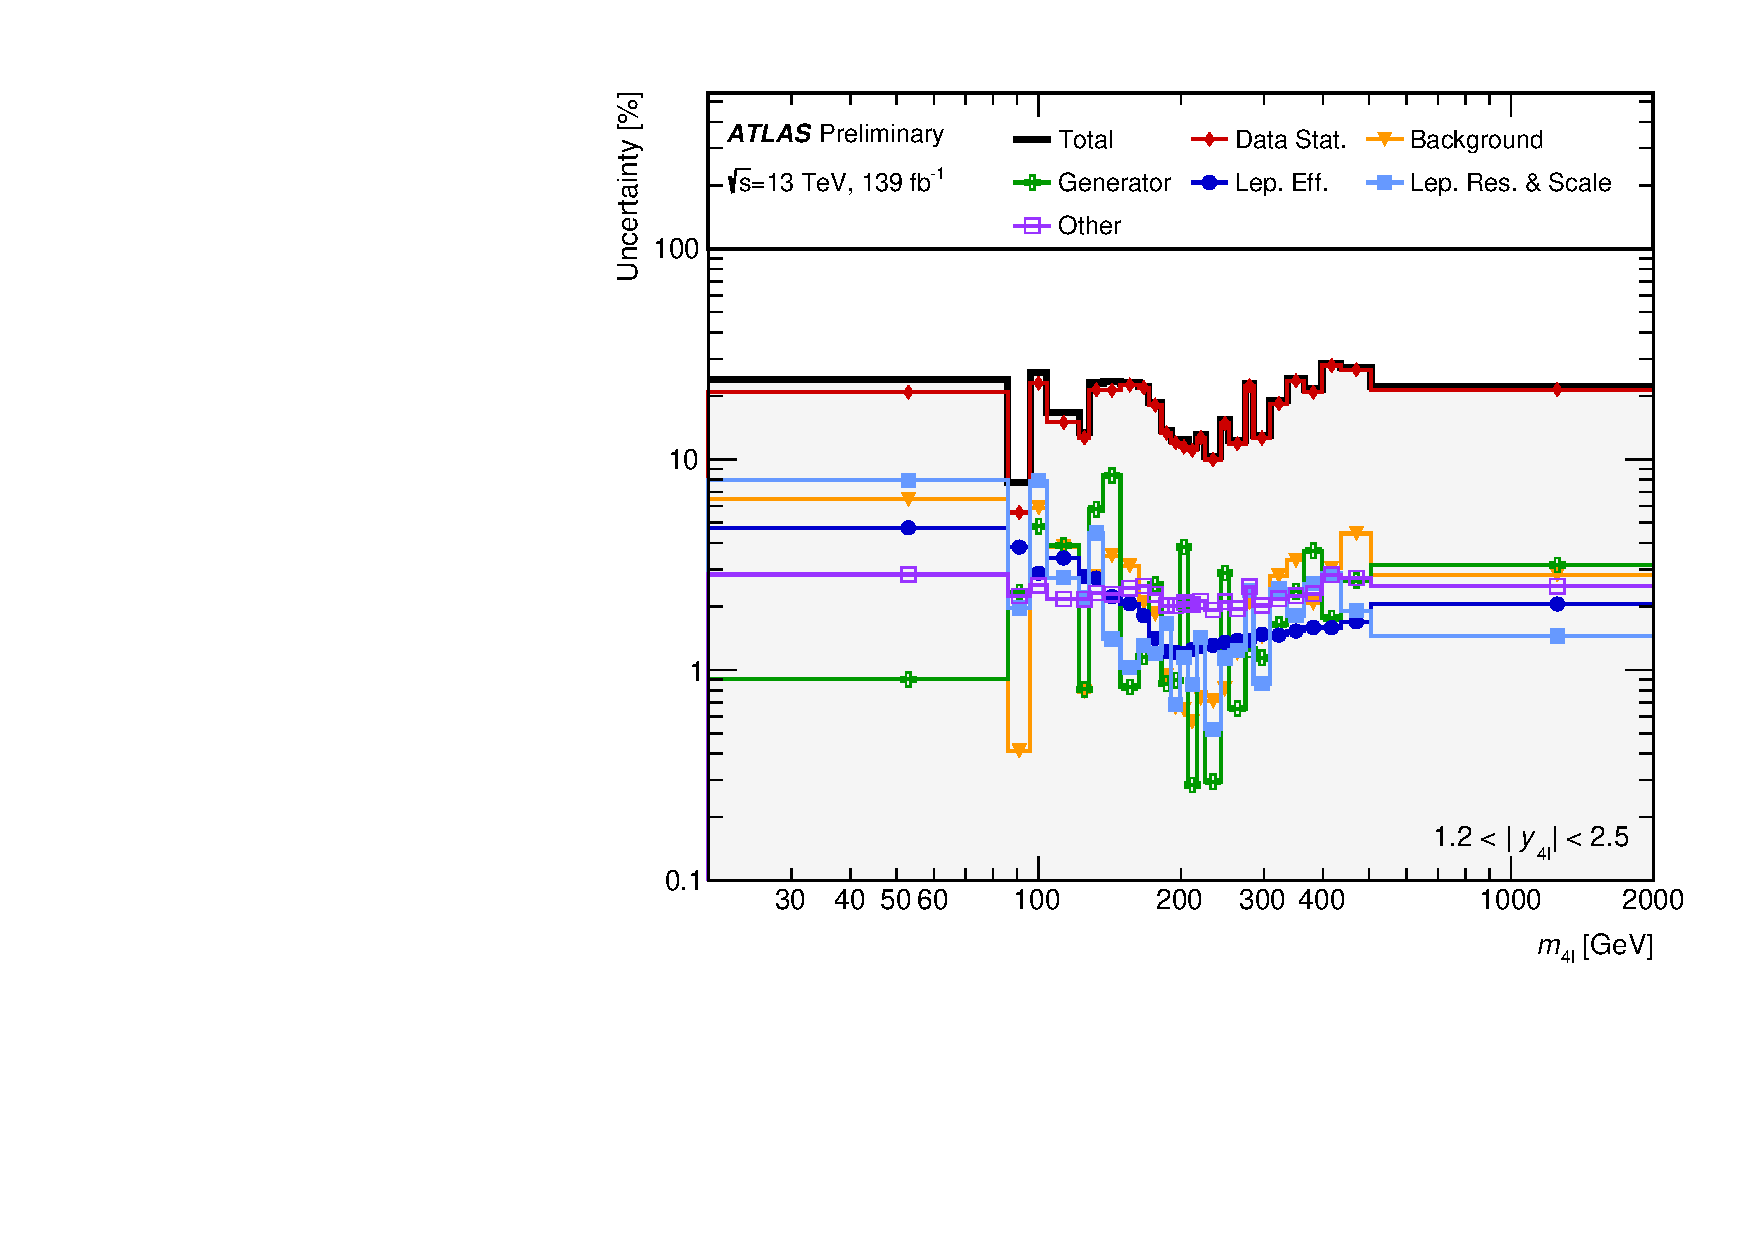
\includegraphics[width = 0.95\textwidth]{Figures/m4l/Systematics/Unfolded/UnfoldedSys_M4lvRapiditybin_Stack_Paper4.pdf}\end{subfigure}
    \caption{Unfolded systematics versus $\mFourL$, in slices of $\yFourL$.}
\end{figure}

\begin{figure}[hp]
    \centering
    \begin{subfigure}{.49\textwidth}\centering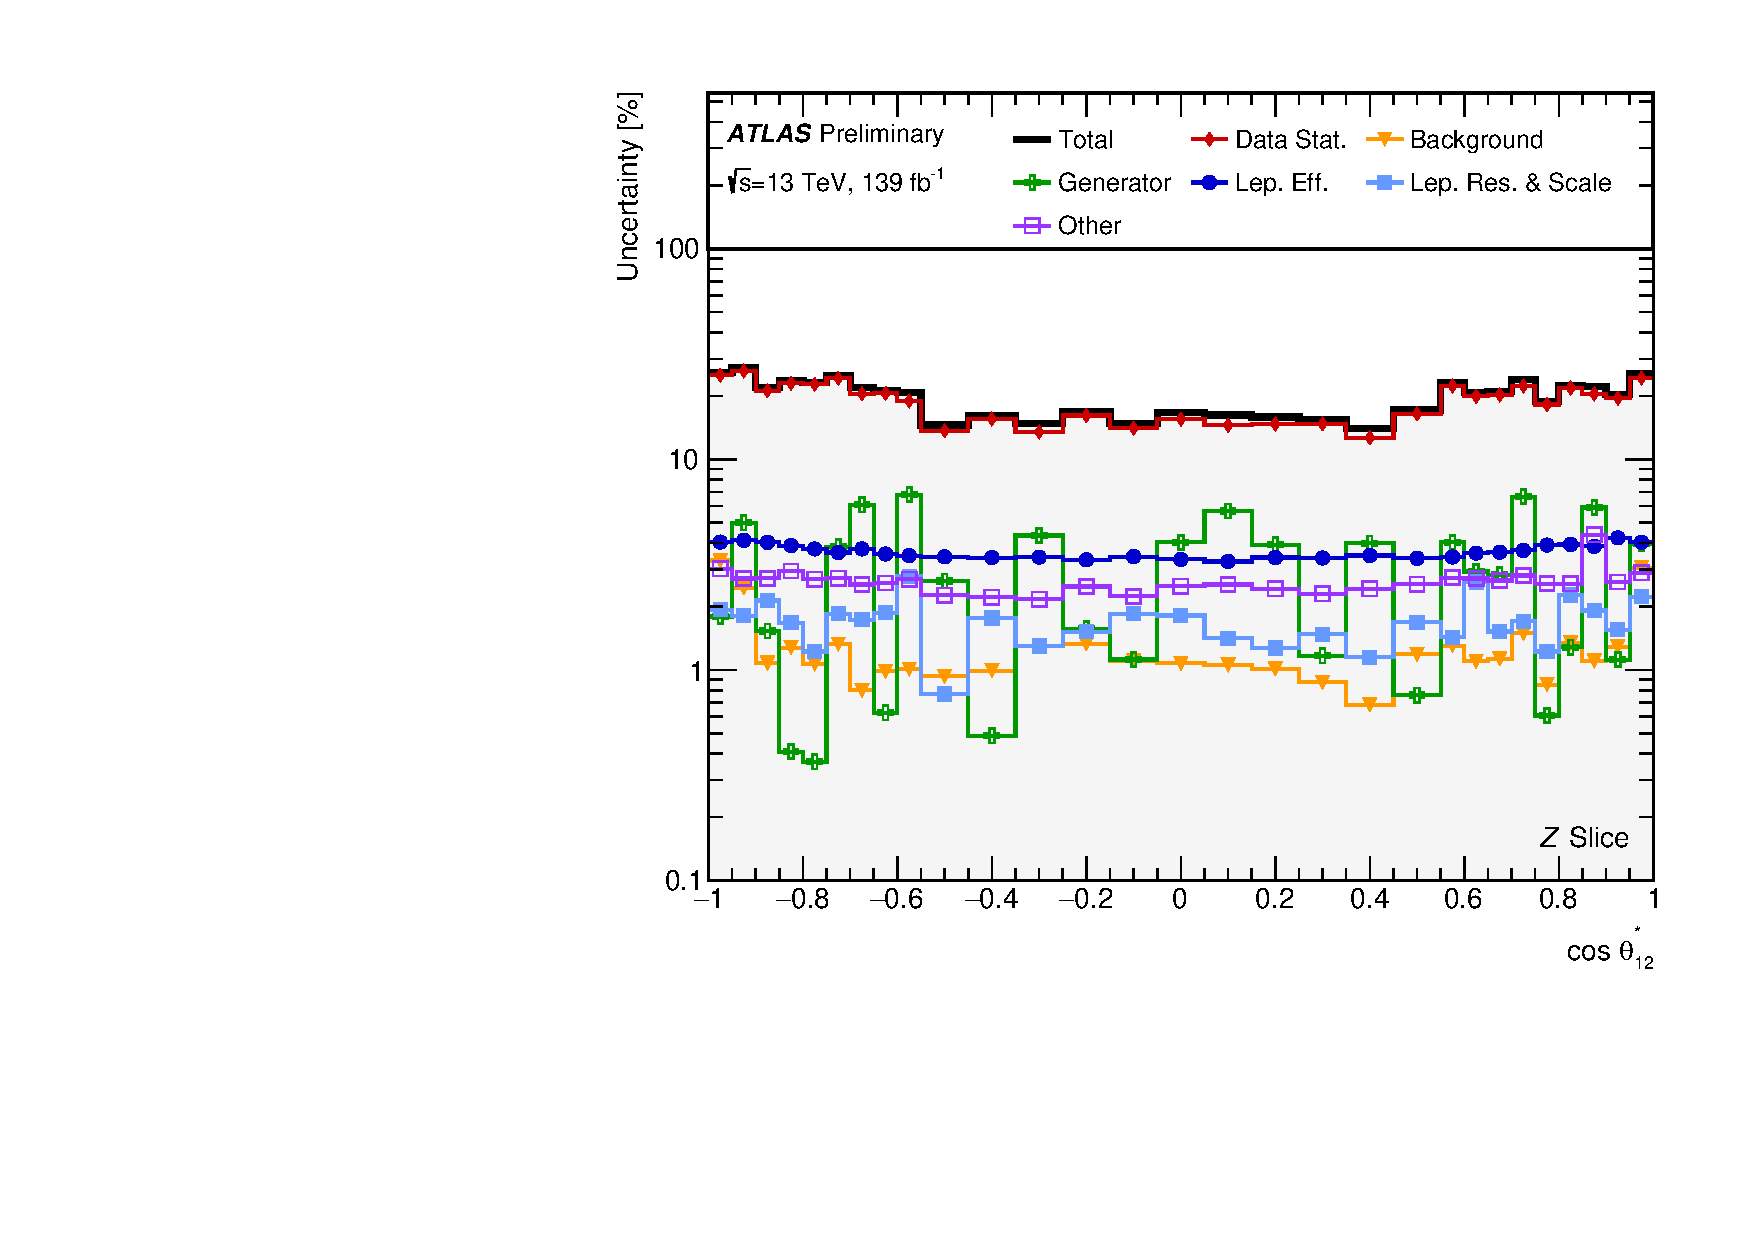
\includegraphics[width = 0.95\textwidth]{Figures/m4l/Systematics/Unfolded/UnfoldedSys_CTS12_vs_M4l_Stack_Paper0.pdf}\end{subfigure}
    \begin{subfigure}{.49\textwidth}\centering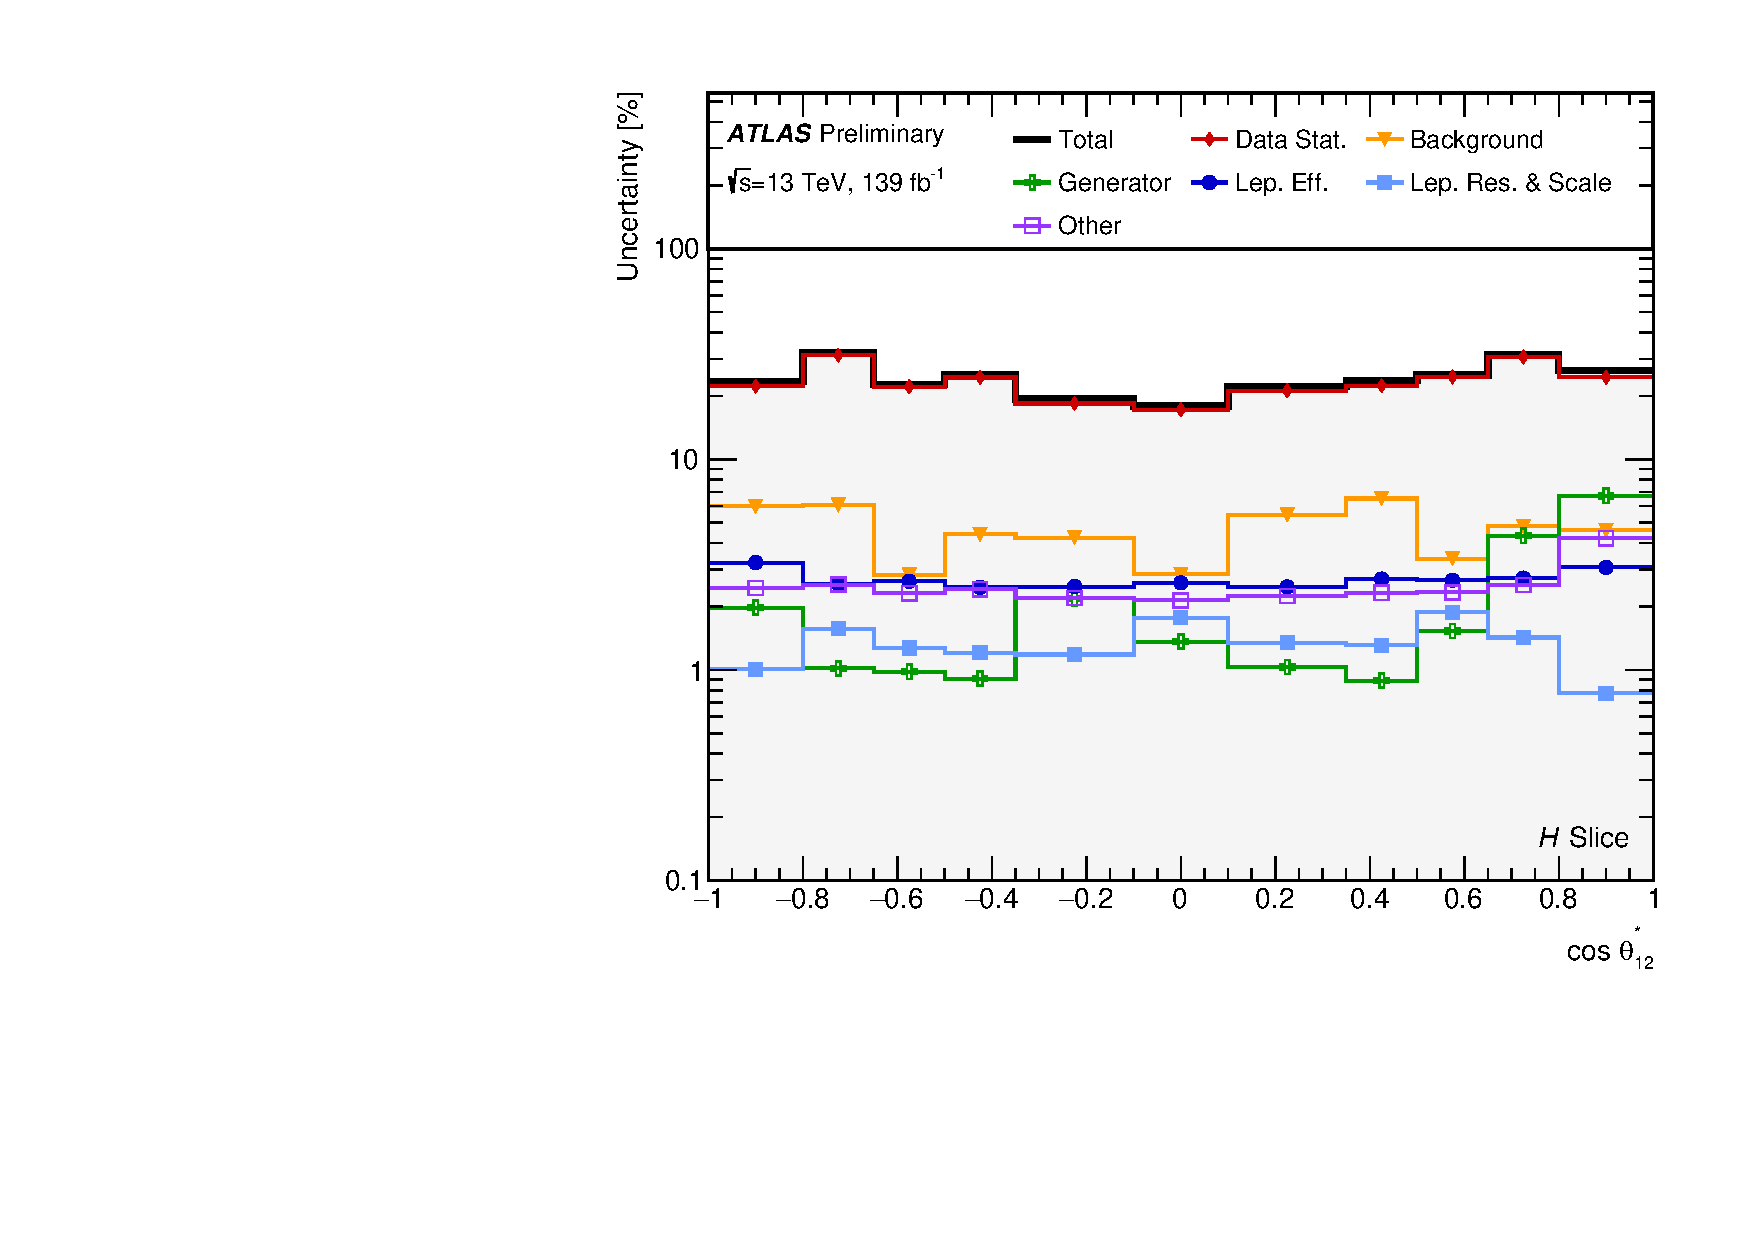
\includegraphics[width = 0.95\textwidth]{Figures/m4l/Systematics/Unfolded/UnfoldedSys_CTS12_vs_M4l_Stack_Paper1.pdf}\end{subfigure}
    \begin{subfigure}{.49\textwidth}\centering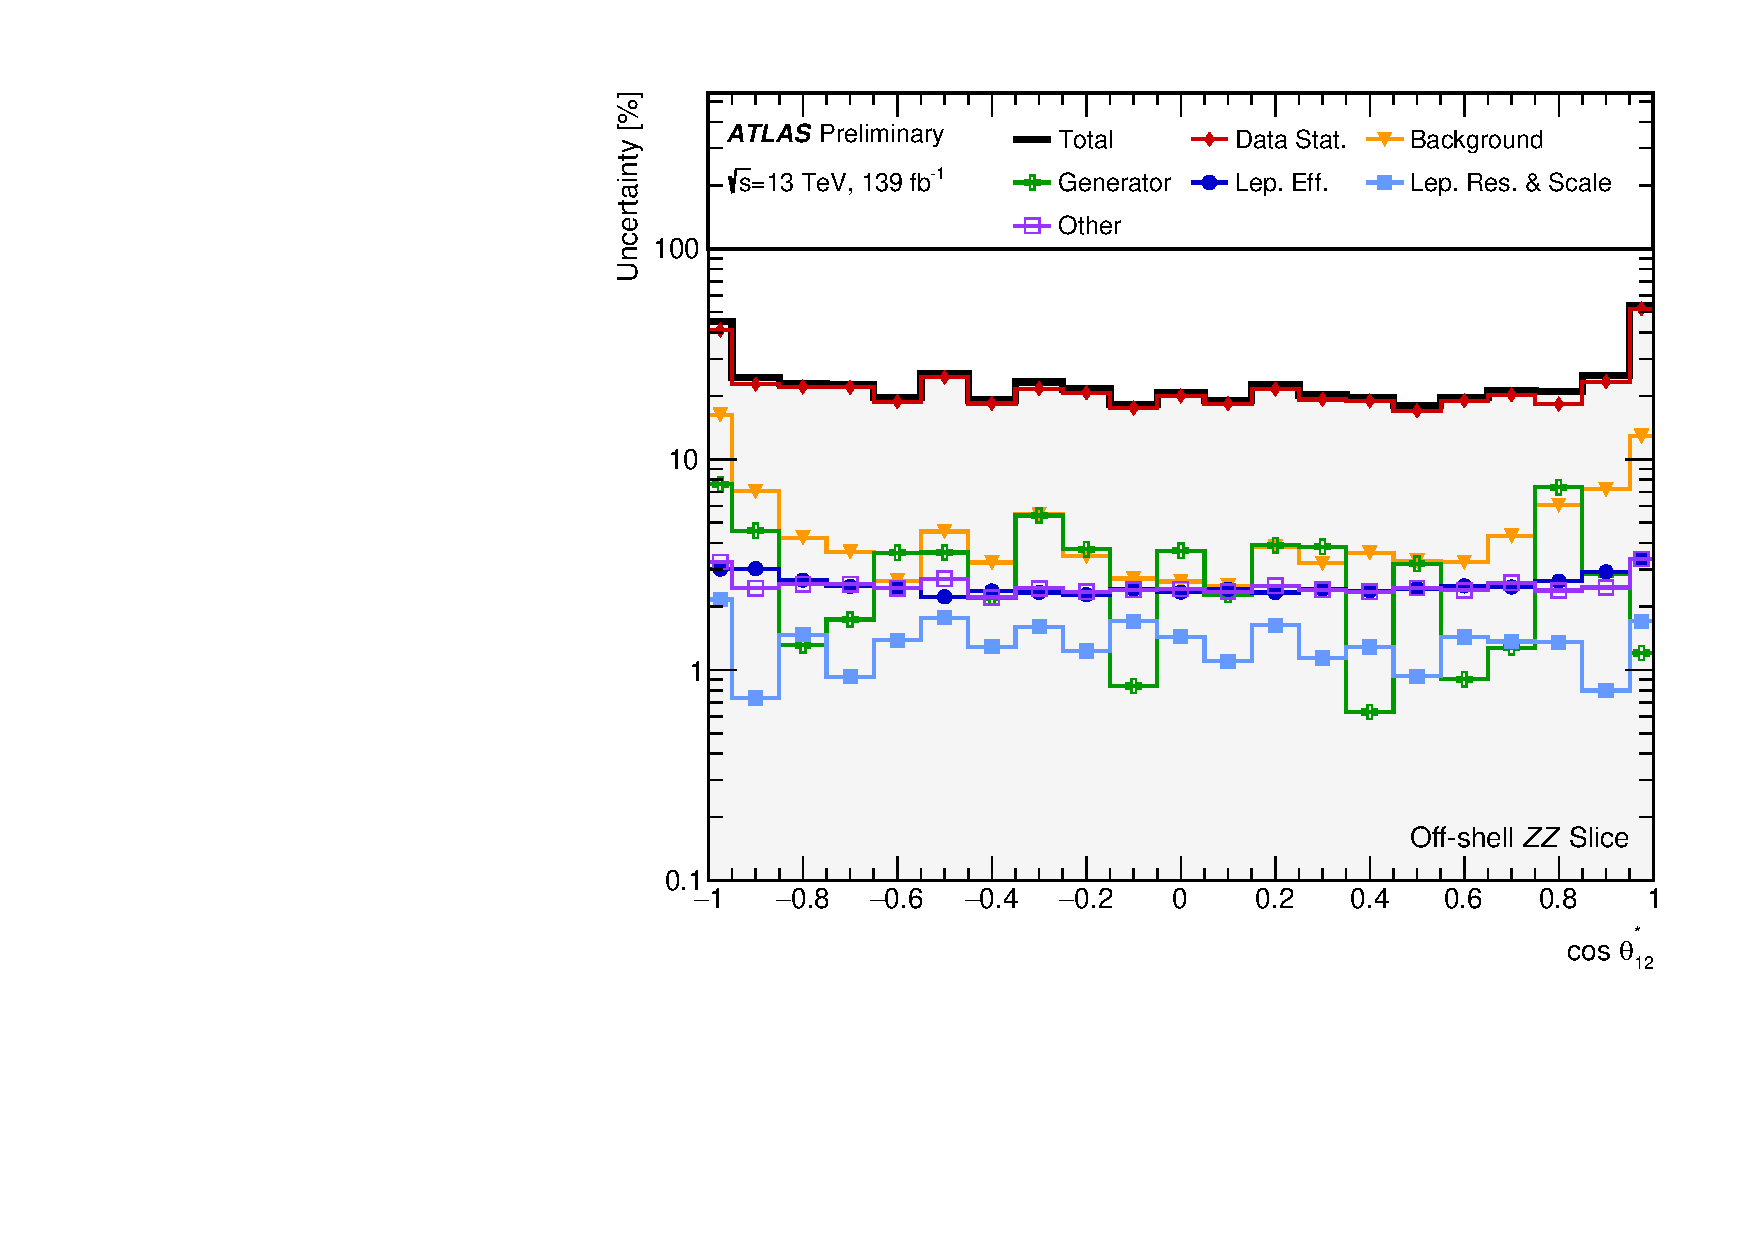
\includegraphics[width = 0.95\textwidth]{Figures/m4l/Systematics/Unfolded/UnfoldedSys_CTS12_vs_M4l_Stack_Paper2.pdf}\end{subfigure}
    \begin{subfigure}{.49\textwidth}\centering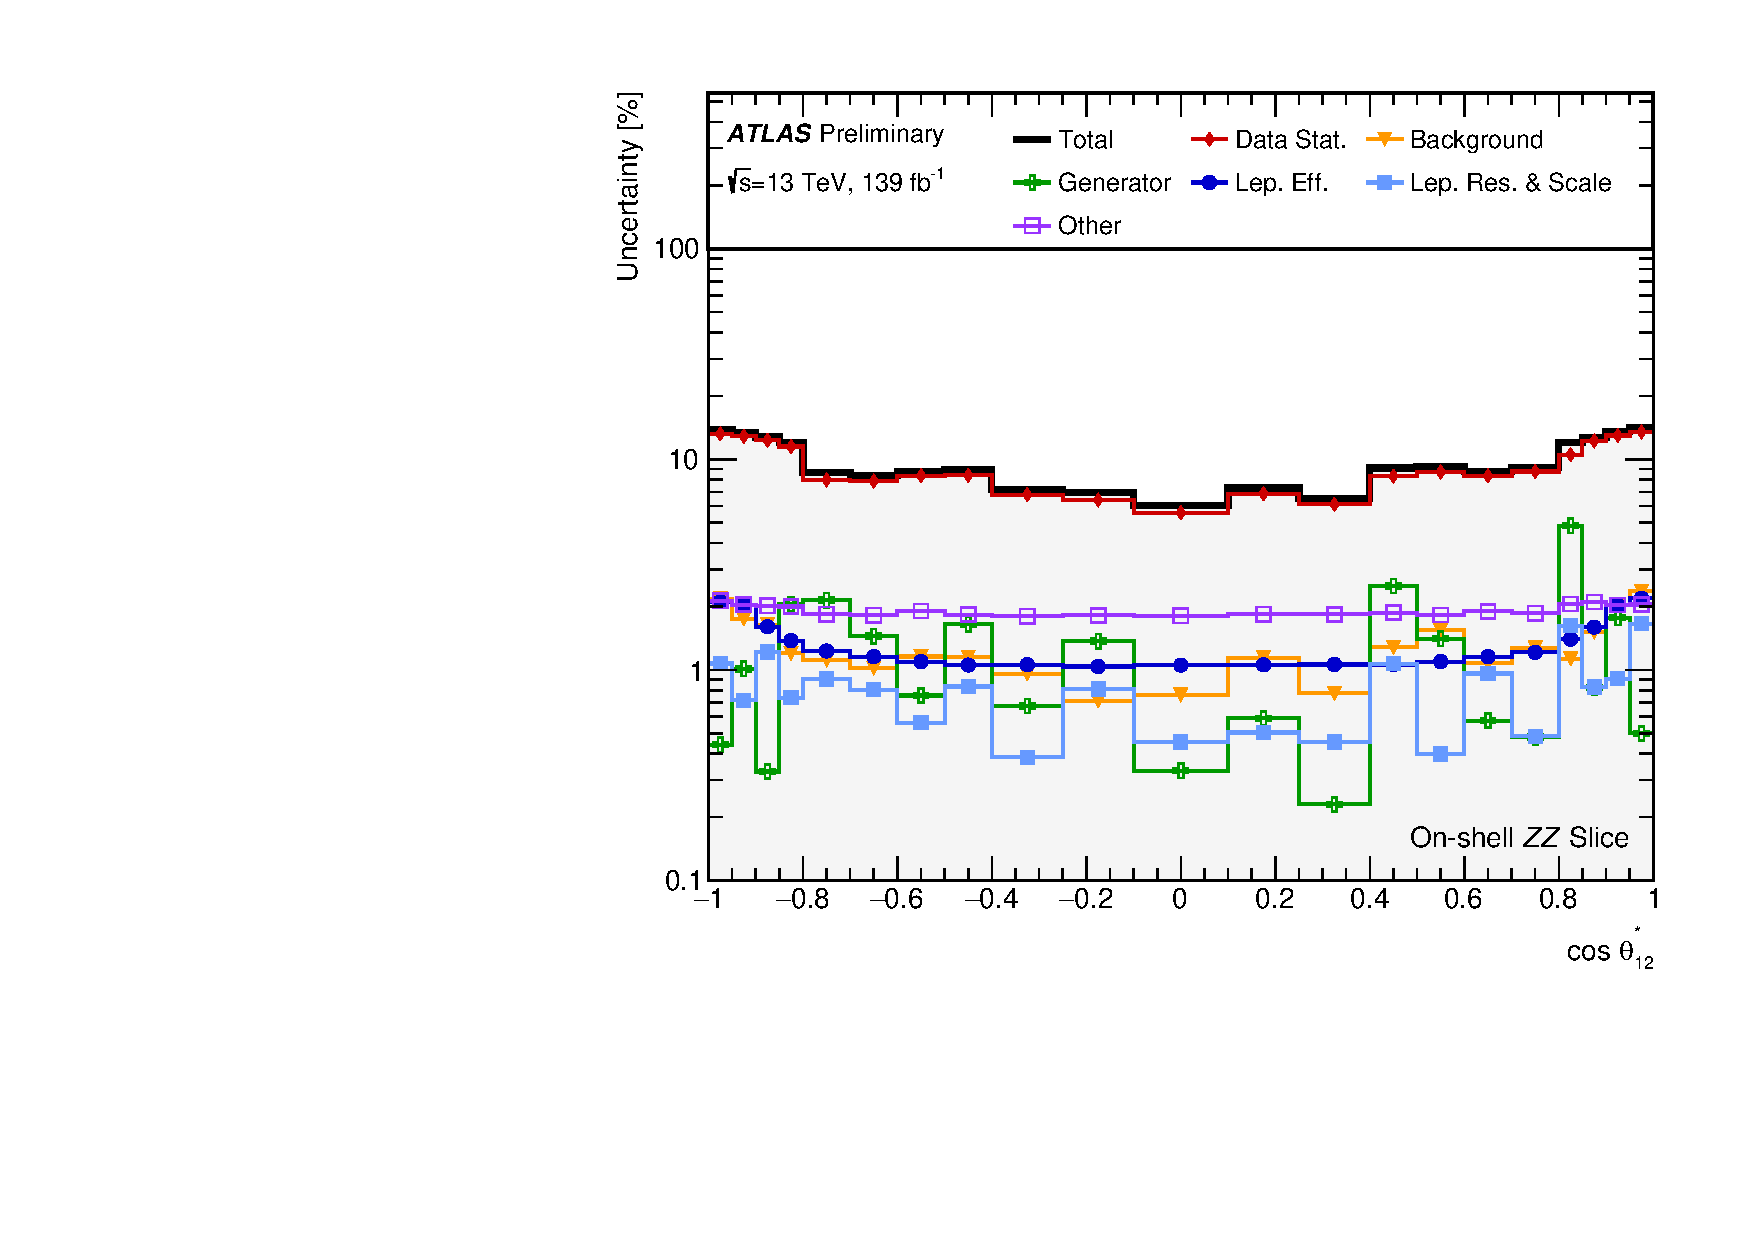
\includegraphics[width = 0.95\textwidth]{Figures/m4l/Systematics/Unfolded/UnfoldedSys_CTS12_vs_M4l_Stack_Paper3.pdf}\end{subfigure}
    \caption{Unfolded systematics versus $\costhetastar_{1}$, in slices of $\mFourL$.}
\end{figure}

\begin{figure}[hp]
    \centering
    \begin{subfigure}{.49\textwidth}\centering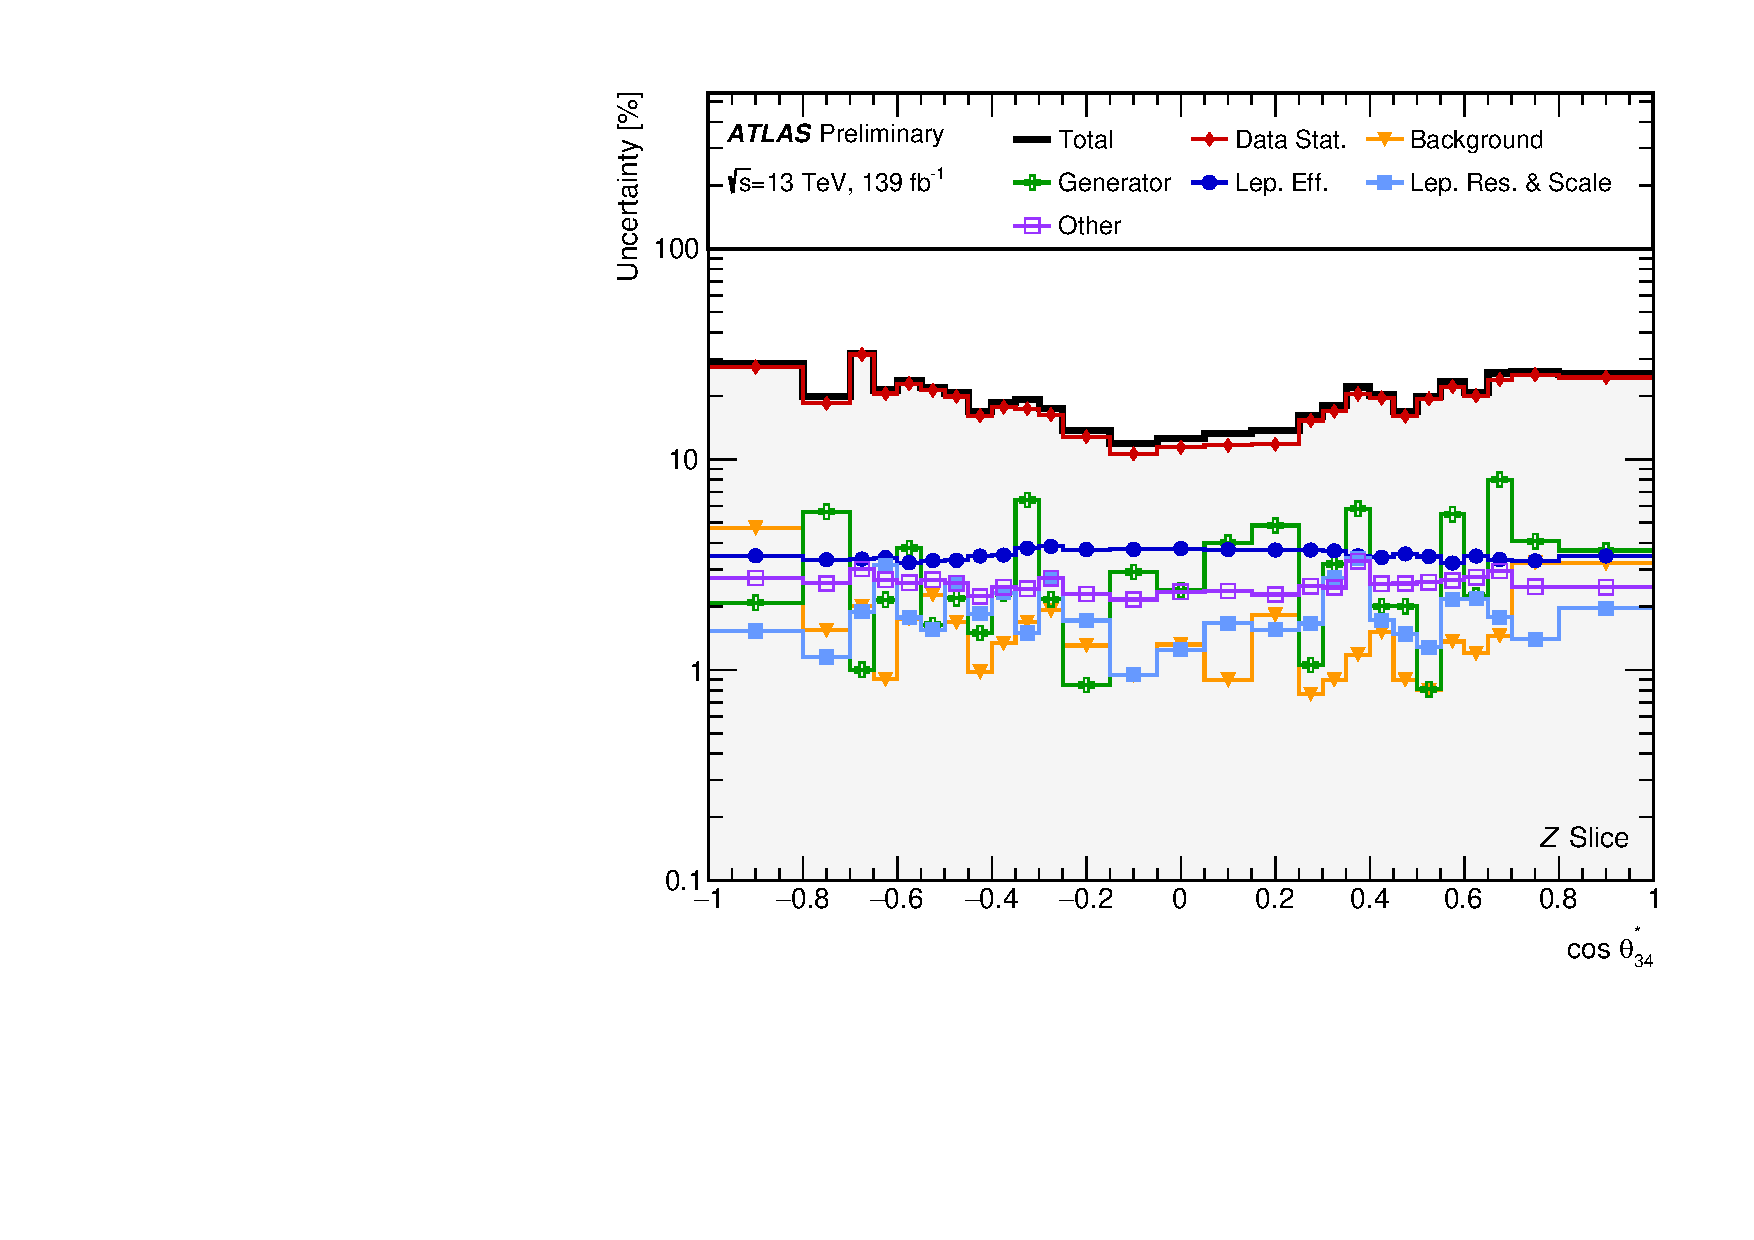
\includegraphics[width = 0.95\textwidth]{Figures/m4l/Systematics/Unfolded/UnfoldedSys_CTS34_vs_M4l_Stack_Paper0.pdf}\end{subfigure}
    \begin{subfigure}{.49\textwidth}\centering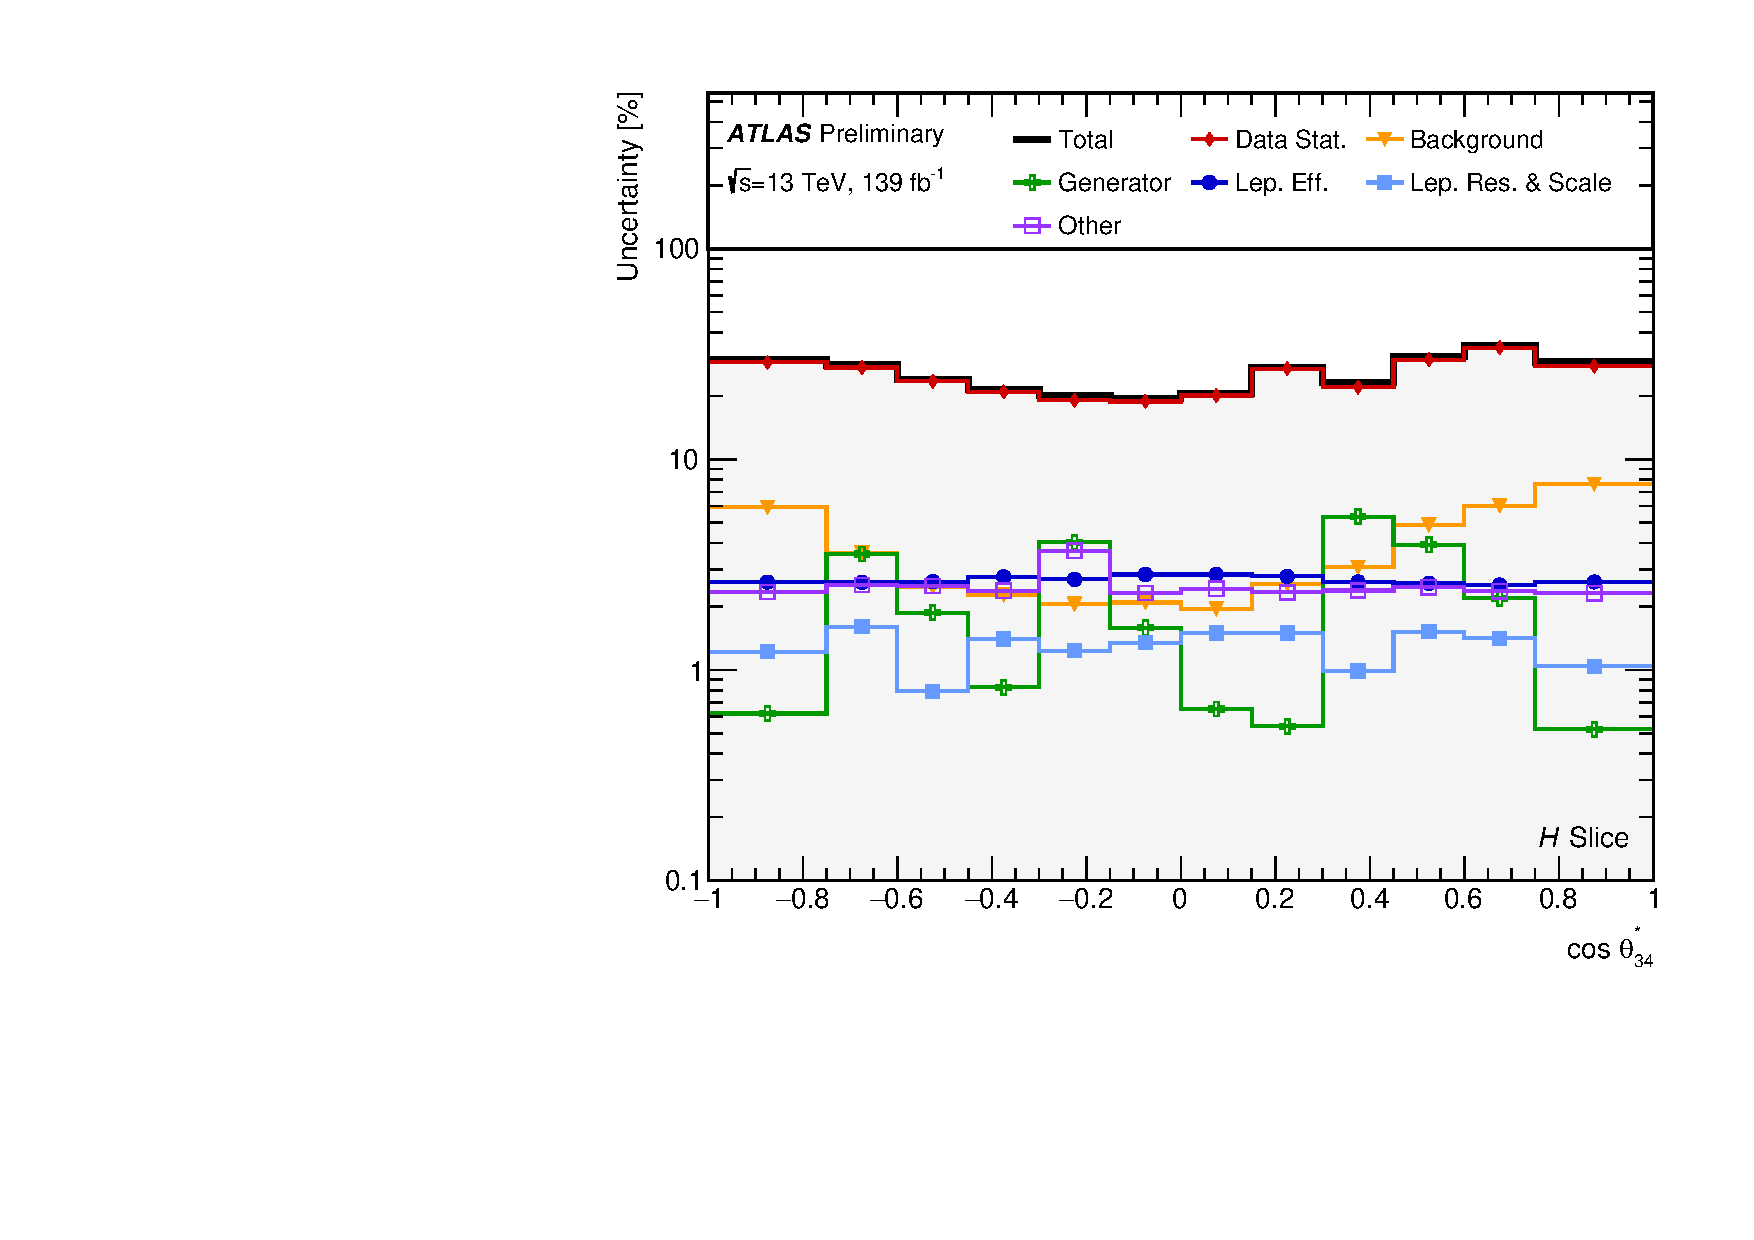
\includegraphics[width = 0.95\textwidth]{Figures/m4l/Systematics/Unfolded/UnfoldedSys_CTS34_vs_M4l_Stack_Paper1.pdf}\end{subfigure}
    \begin{subfigure}{.49\textwidth}\centering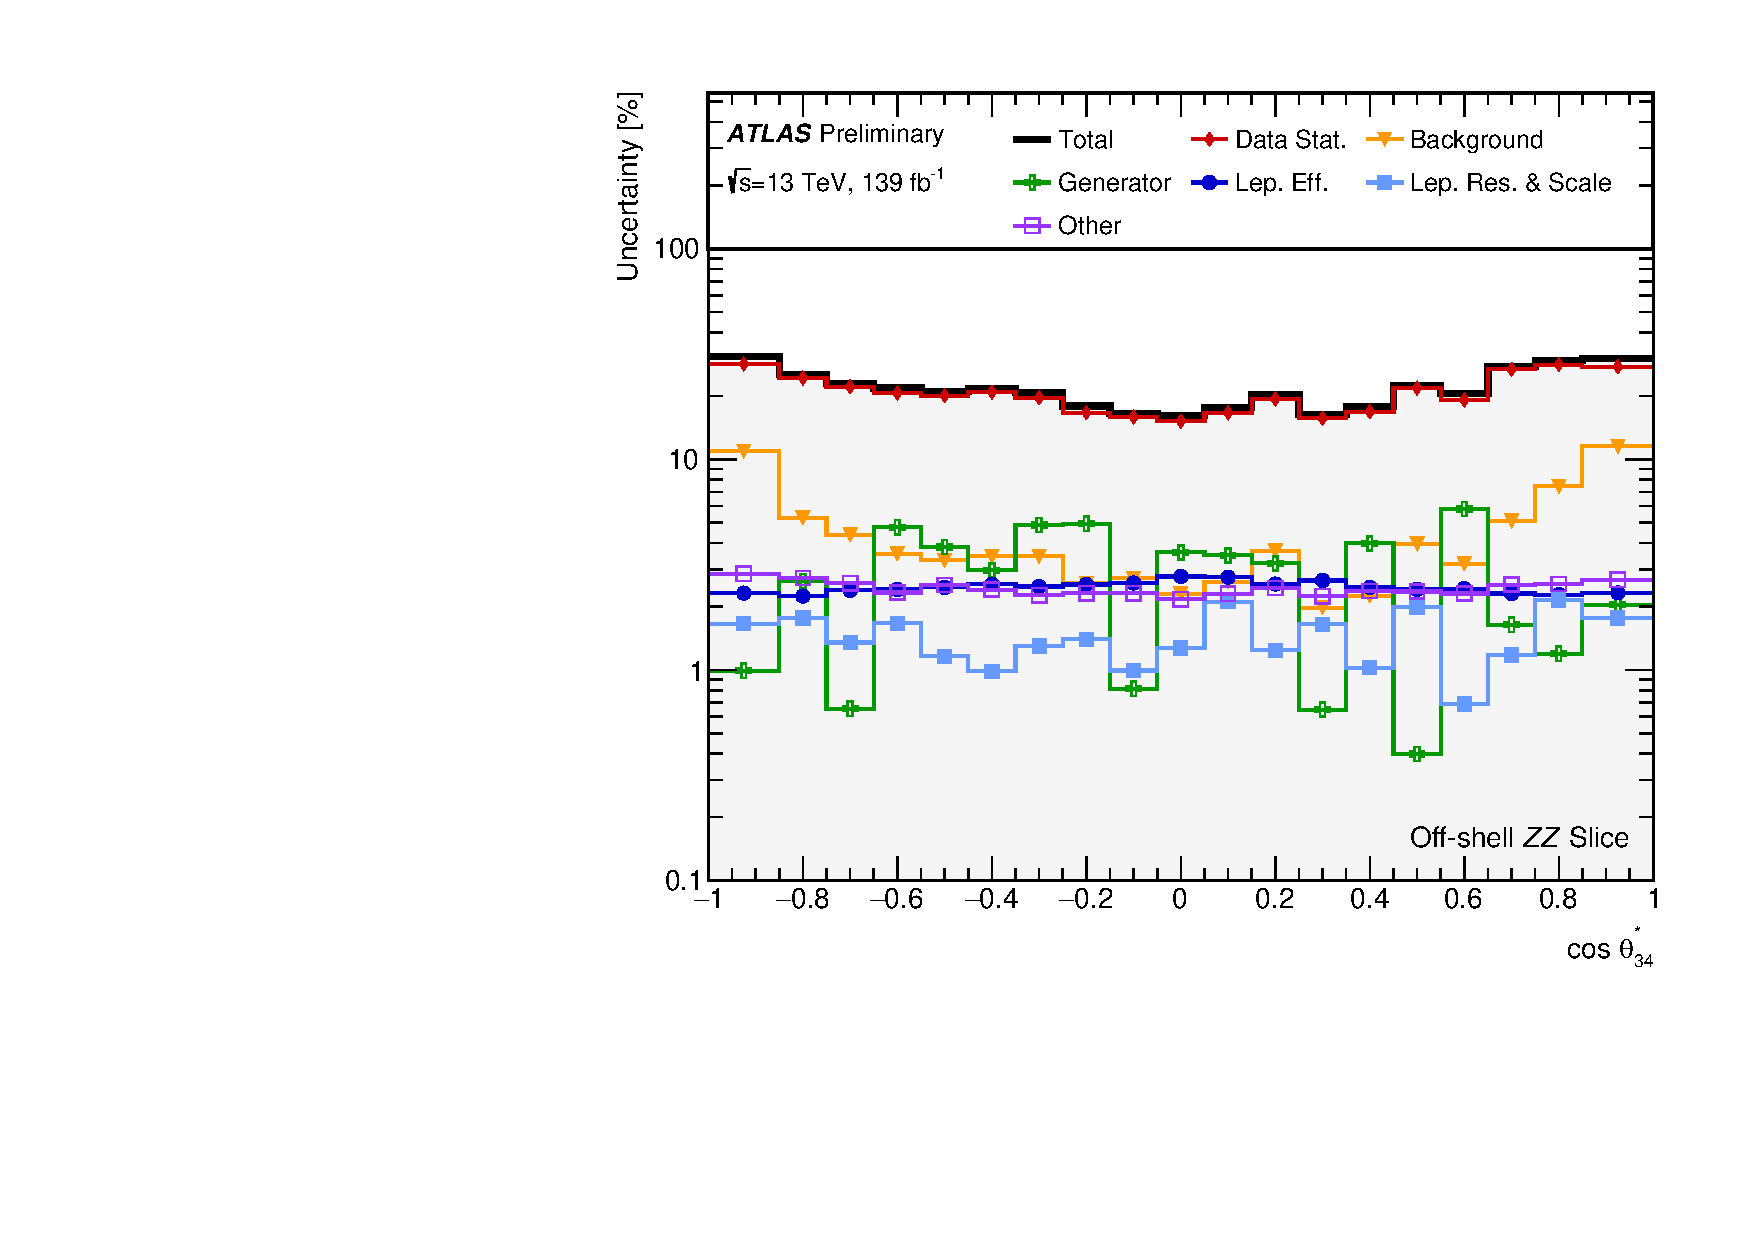
\includegraphics[width = 0.95\textwidth]{Figures/m4l/Systematics/Unfolded/UnfoldedSys_CTS34_vs_M4l_Stack_Paper2.pdf}\end{subfigure}
    \begin{subfigure}{.49\textwidth}\centering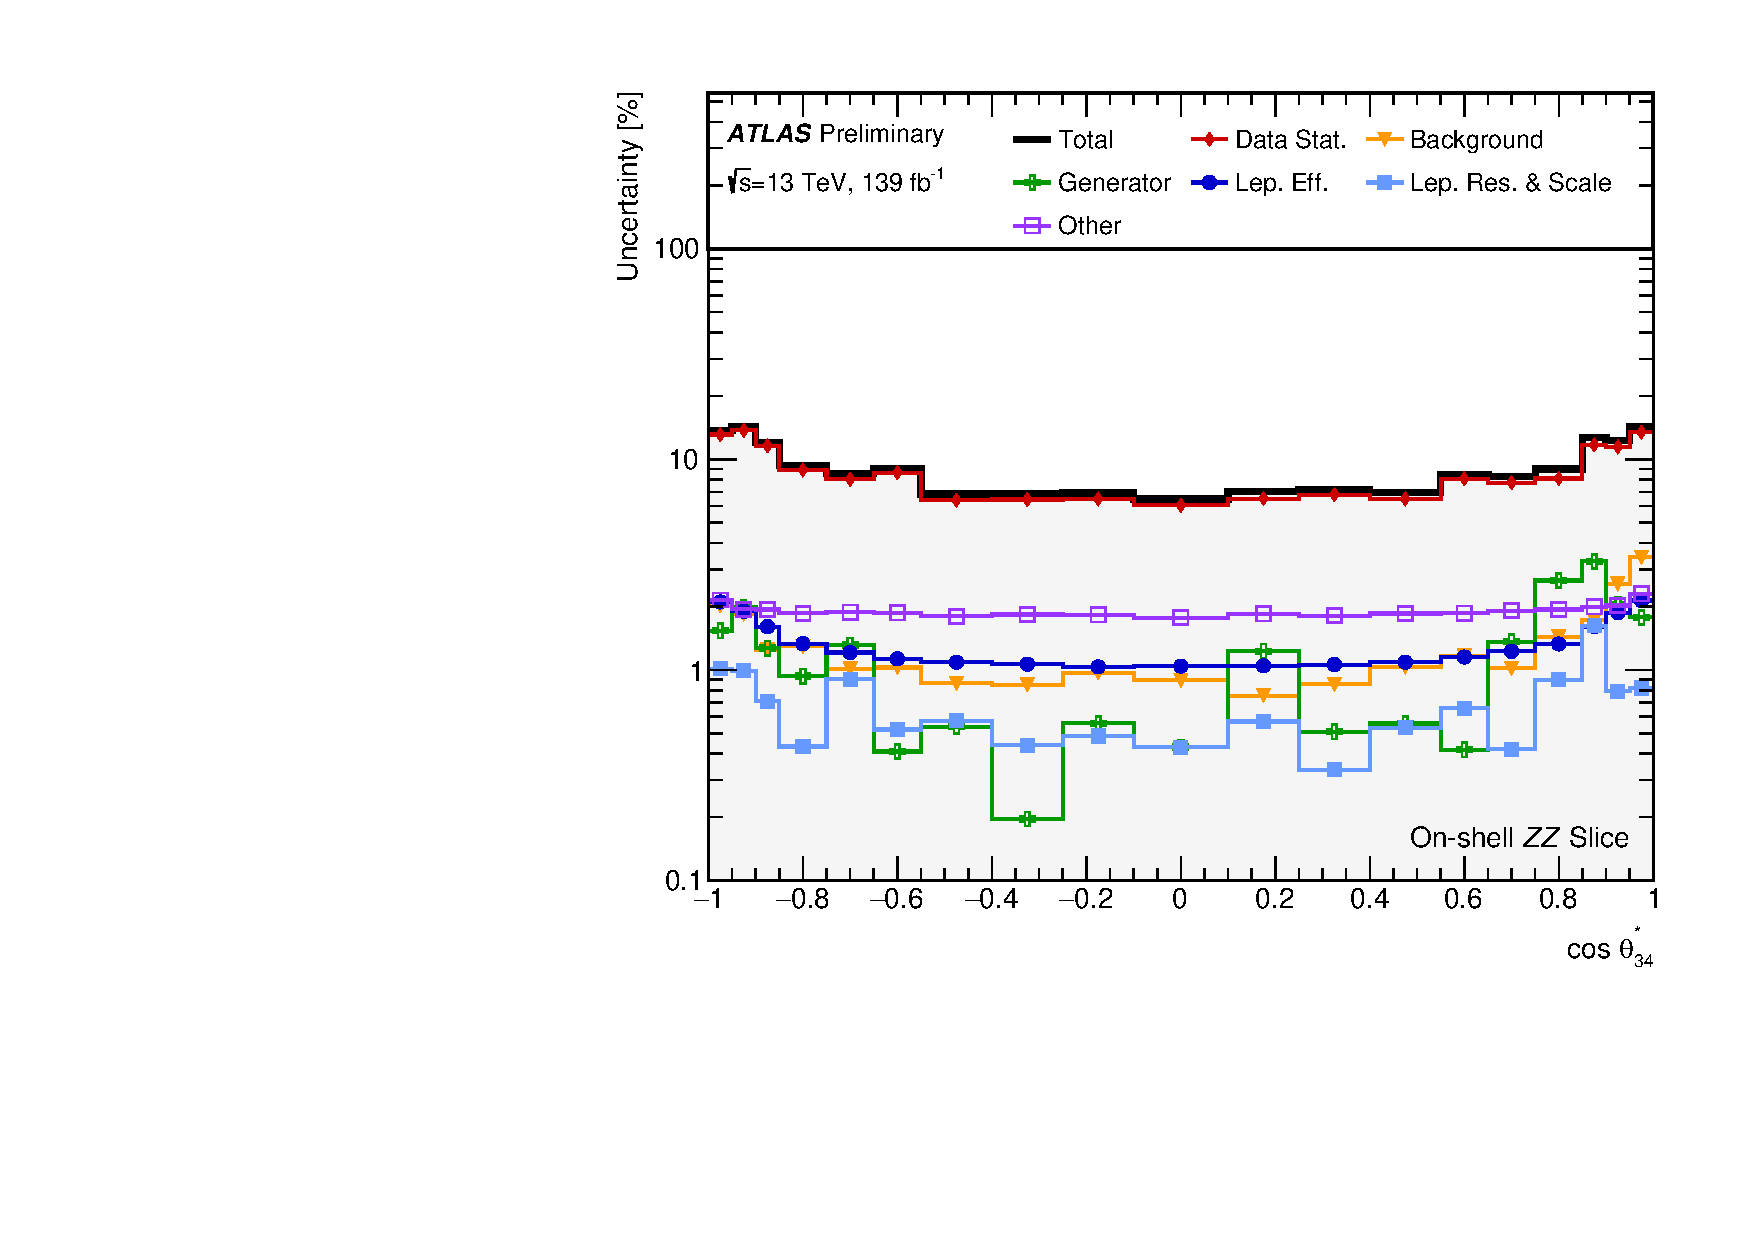
\includegraphics[width = 0.95\textwidth]{Figures/m4l/Systematics/Unfolded/UnfoldedSys_CTS34_vs_M4l_Stack_Paper3.pdf}\end{subfigure}
    \caption{Unfolded systematics versus $\costhetastar_{2}$, in slices of $\mFourL$.}
\end{figure}

\begin{figure}[hp]
    \centering
    \begin{subfigure}{.49\textwidth}\centering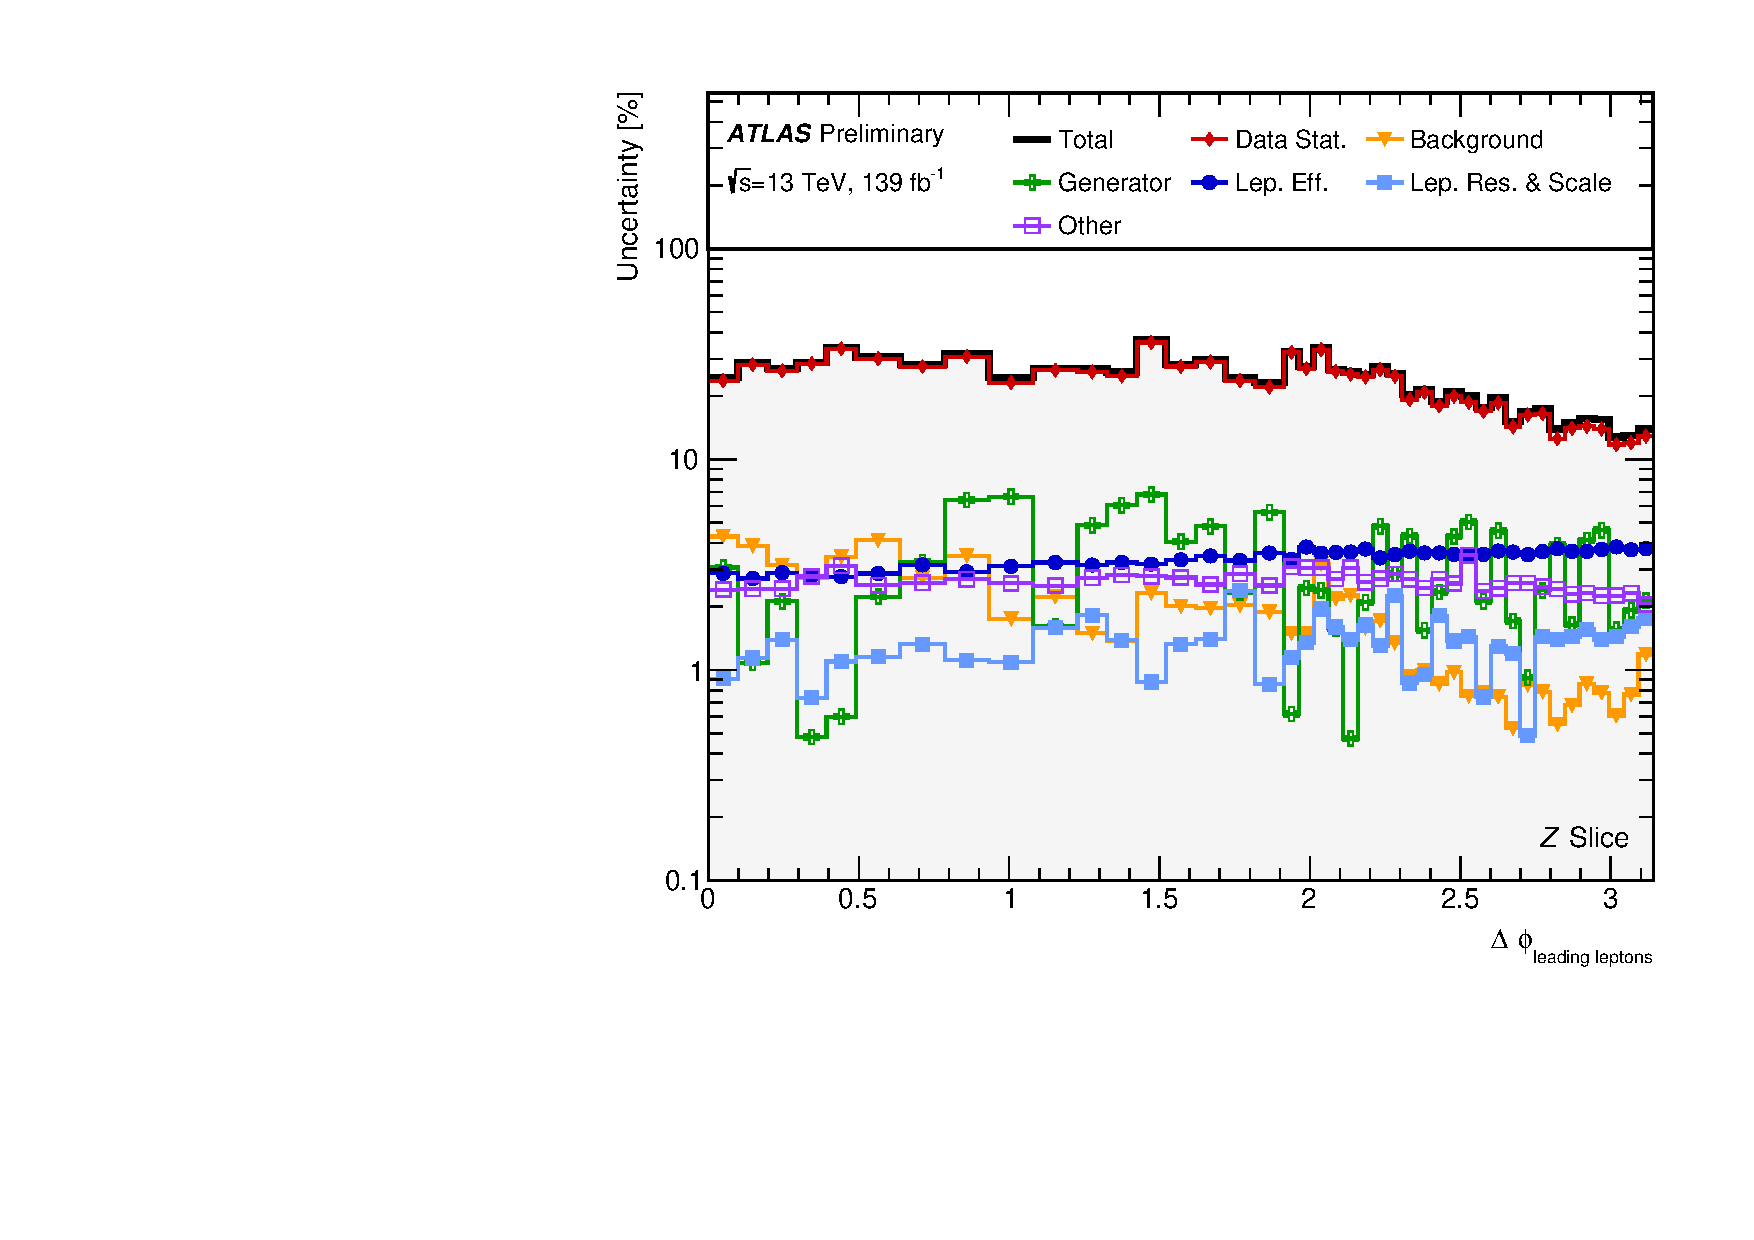
\includegraphics[width = 0.95\textwidth]{Figures/m4l/Systematics/Unfolded/UnfoldedSys_dPhiLeadLep_vs_M4l_Stack_Paper0.pdf}\end{subfigure}
    \begin{subfigure}{.49\textwidth}\centering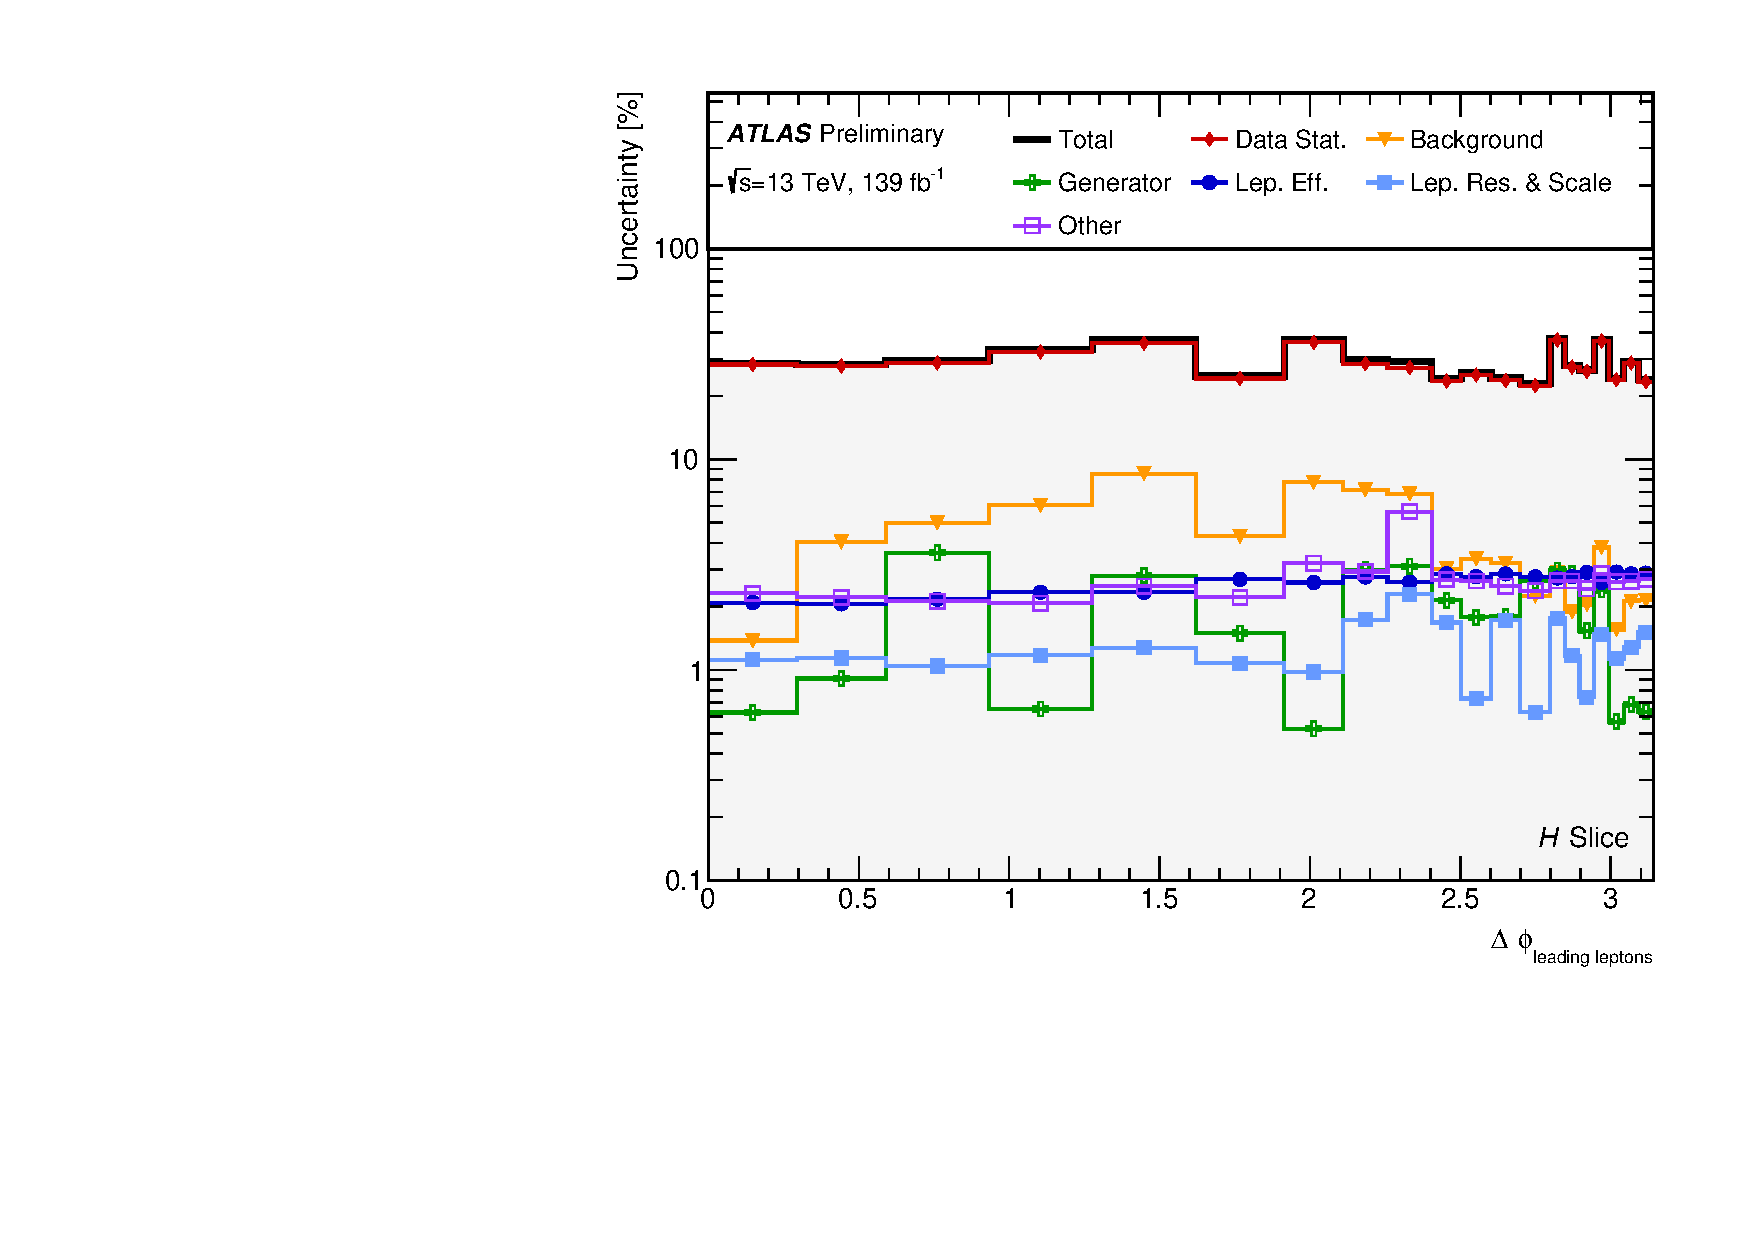
\includegraphics[width = 0.95\textwidth]{Figures/m4l/Systematics/Unfolded/UnfoldedSys_dPhiLeadLep_vs_M4l_Stack_Paper1.pdf}\end{subfigure}
    \begin{subfigure}{.49\textwidth}\centering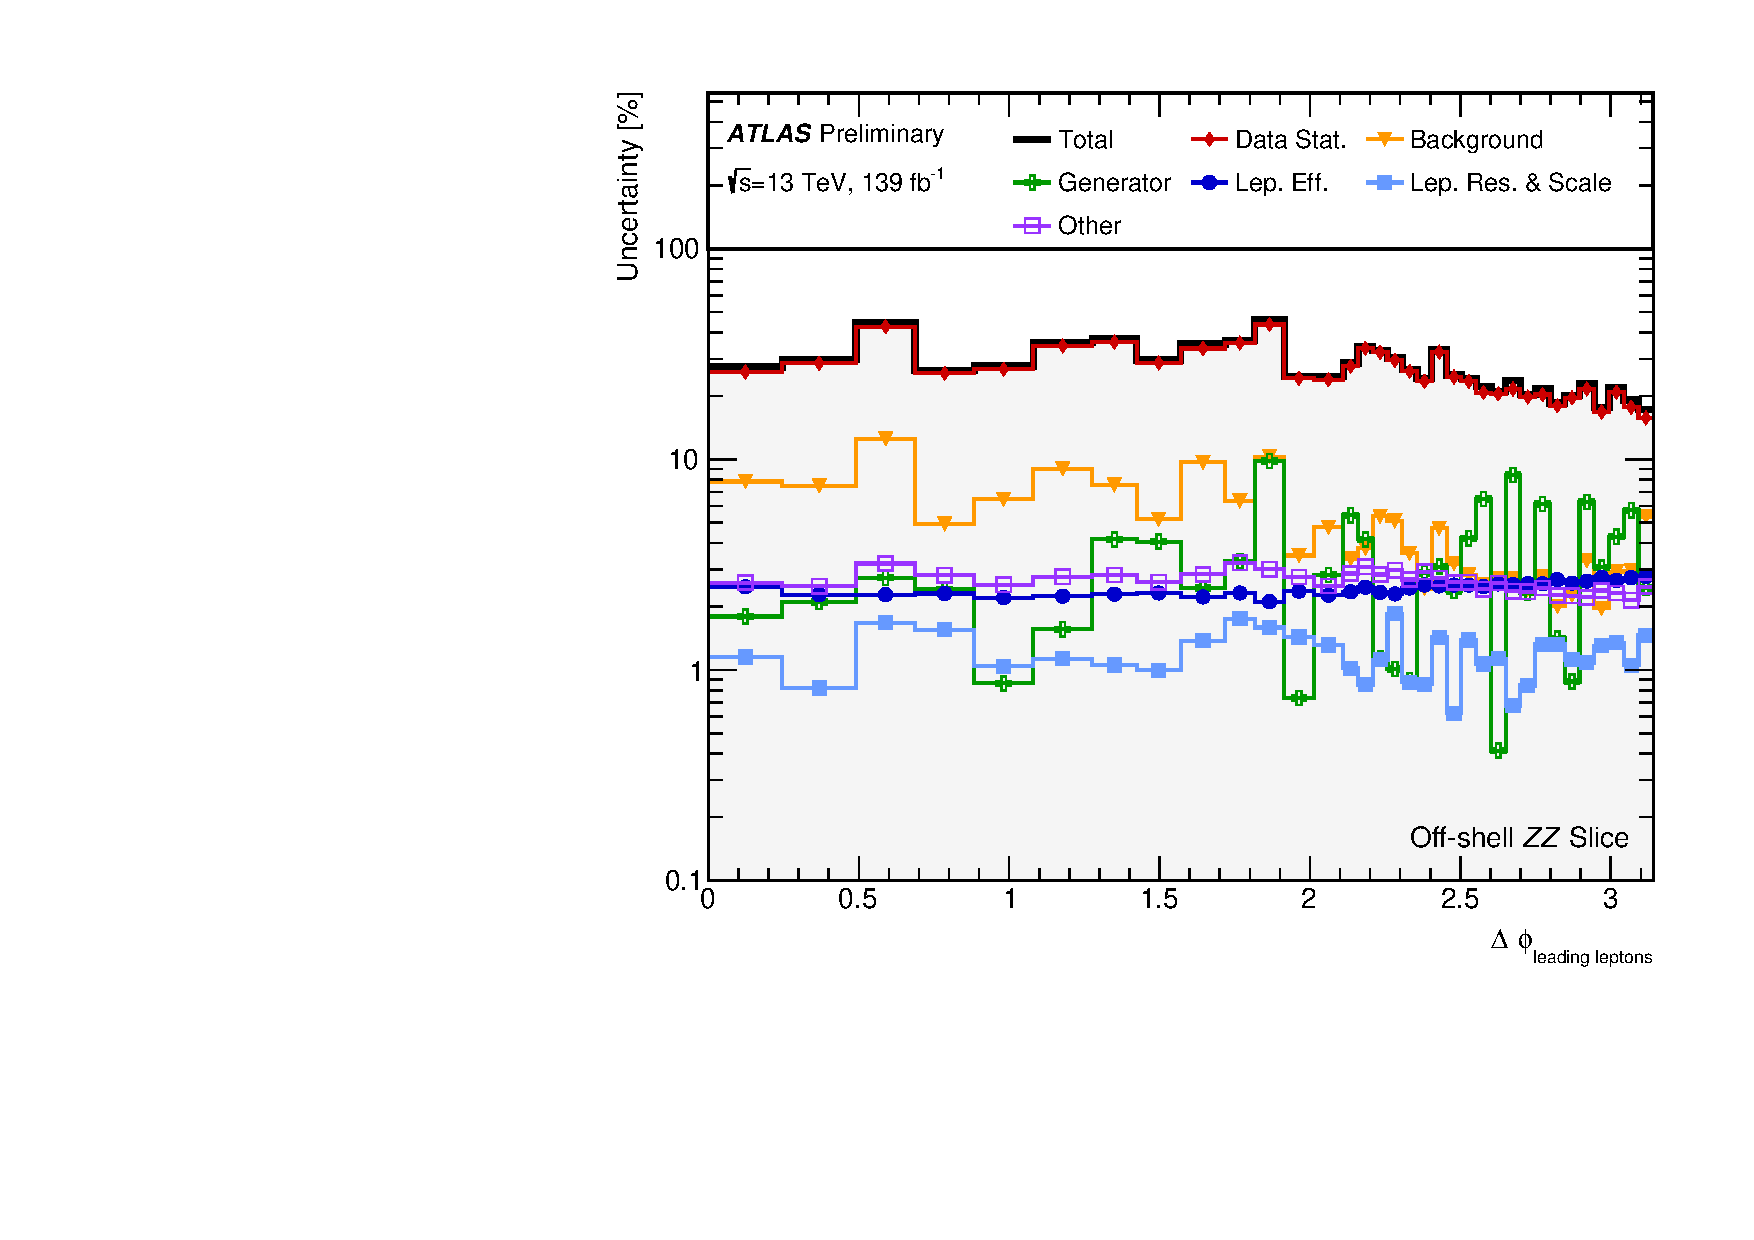
\includegraphics[width = 0.95\textwidth]{Figures/m4l/Systematics/Unfolded/UnfoldedSys_dPhiLeadLep_vs_M4l_Stack_Paper2.pdf}\end{subfigure}
    \begin{subfigure}{.49\textwidth}\centering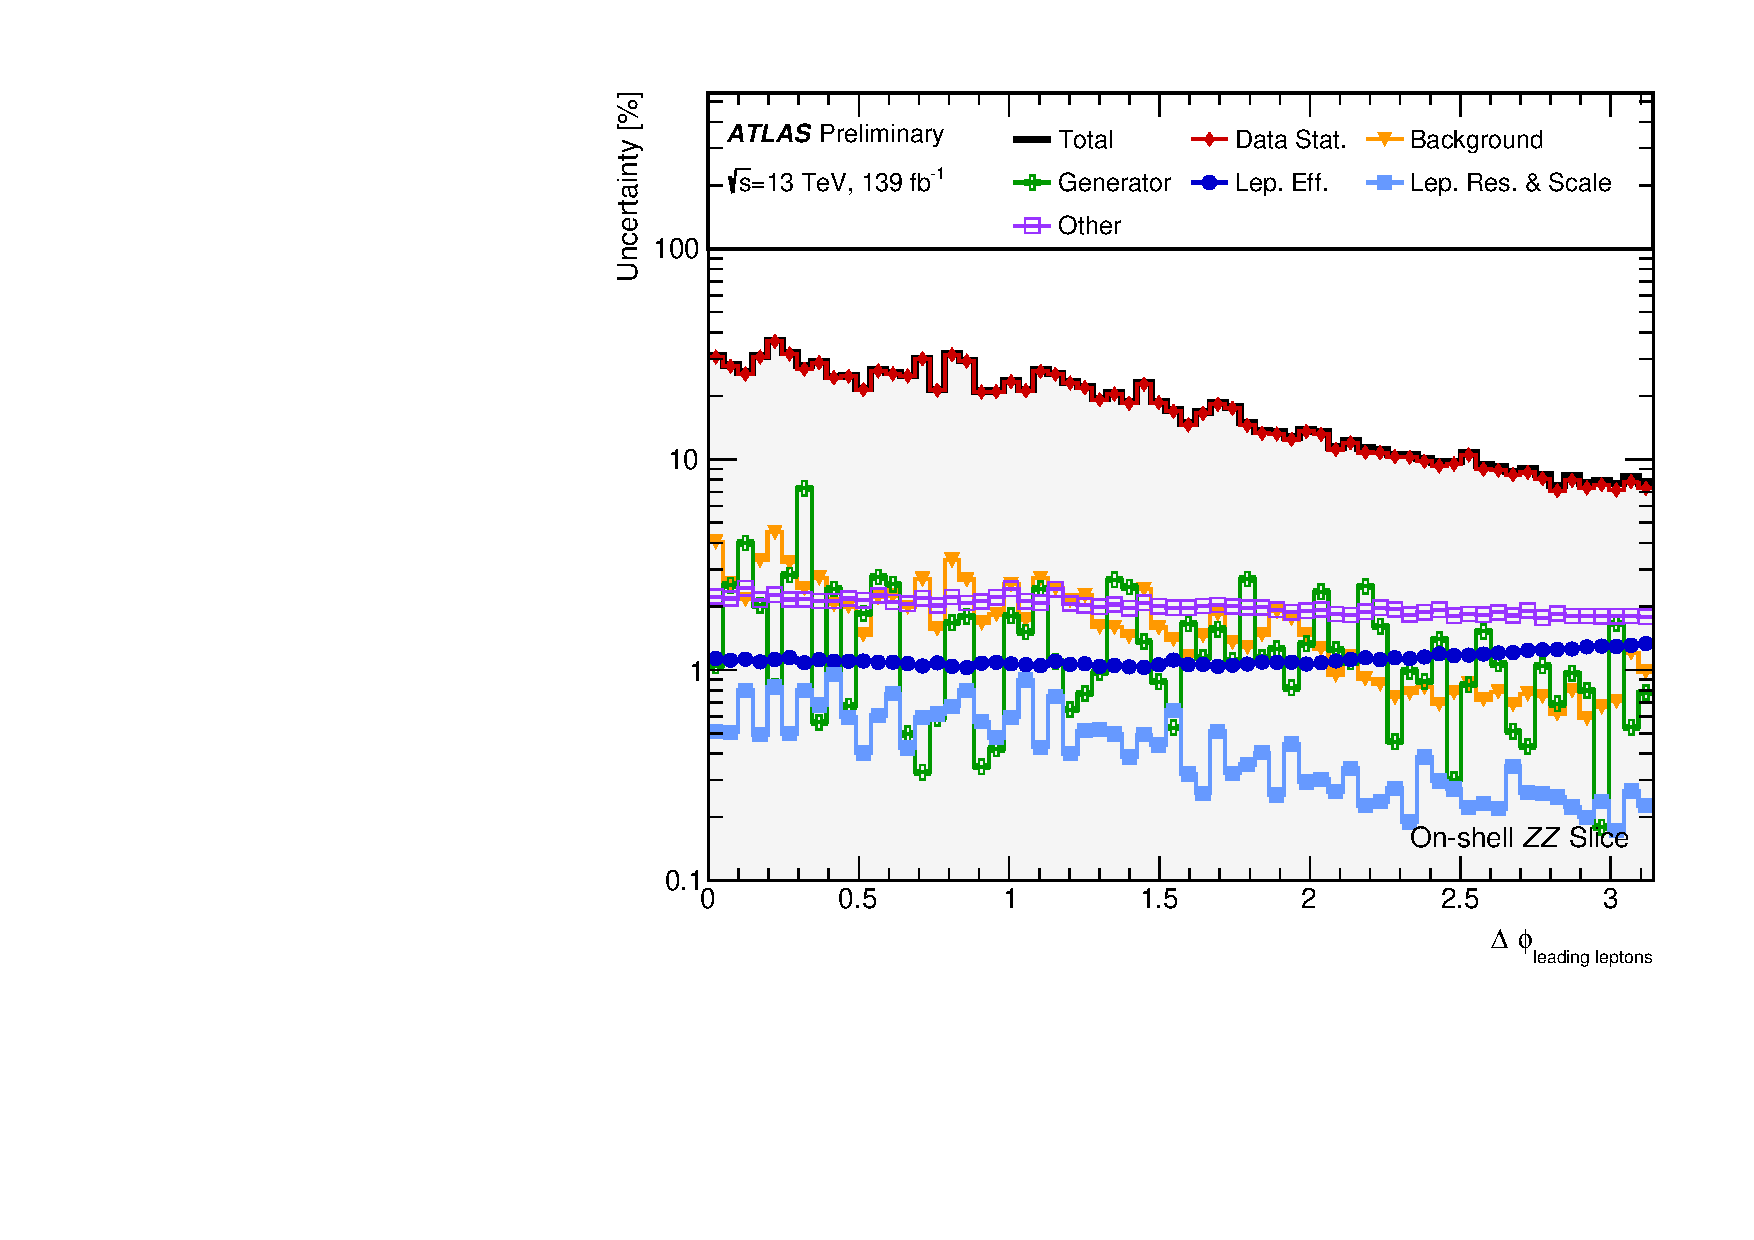
\includegraphics[width = 0.95\textwidth]{Figures/m4l/Systematics/Unfolded/UnfoldedSys_dPhiLeadLep_vs_M4l_Stack_Paper3.pdf}\end{subfigure}
    \caption{Unfolded systematics versus $\dPhill$, in slices of $\mFourL$.}
\end{figure}

\begin{figure}[hp]
    \centering
    \begin{subfigure}{.49\textwidth}\centering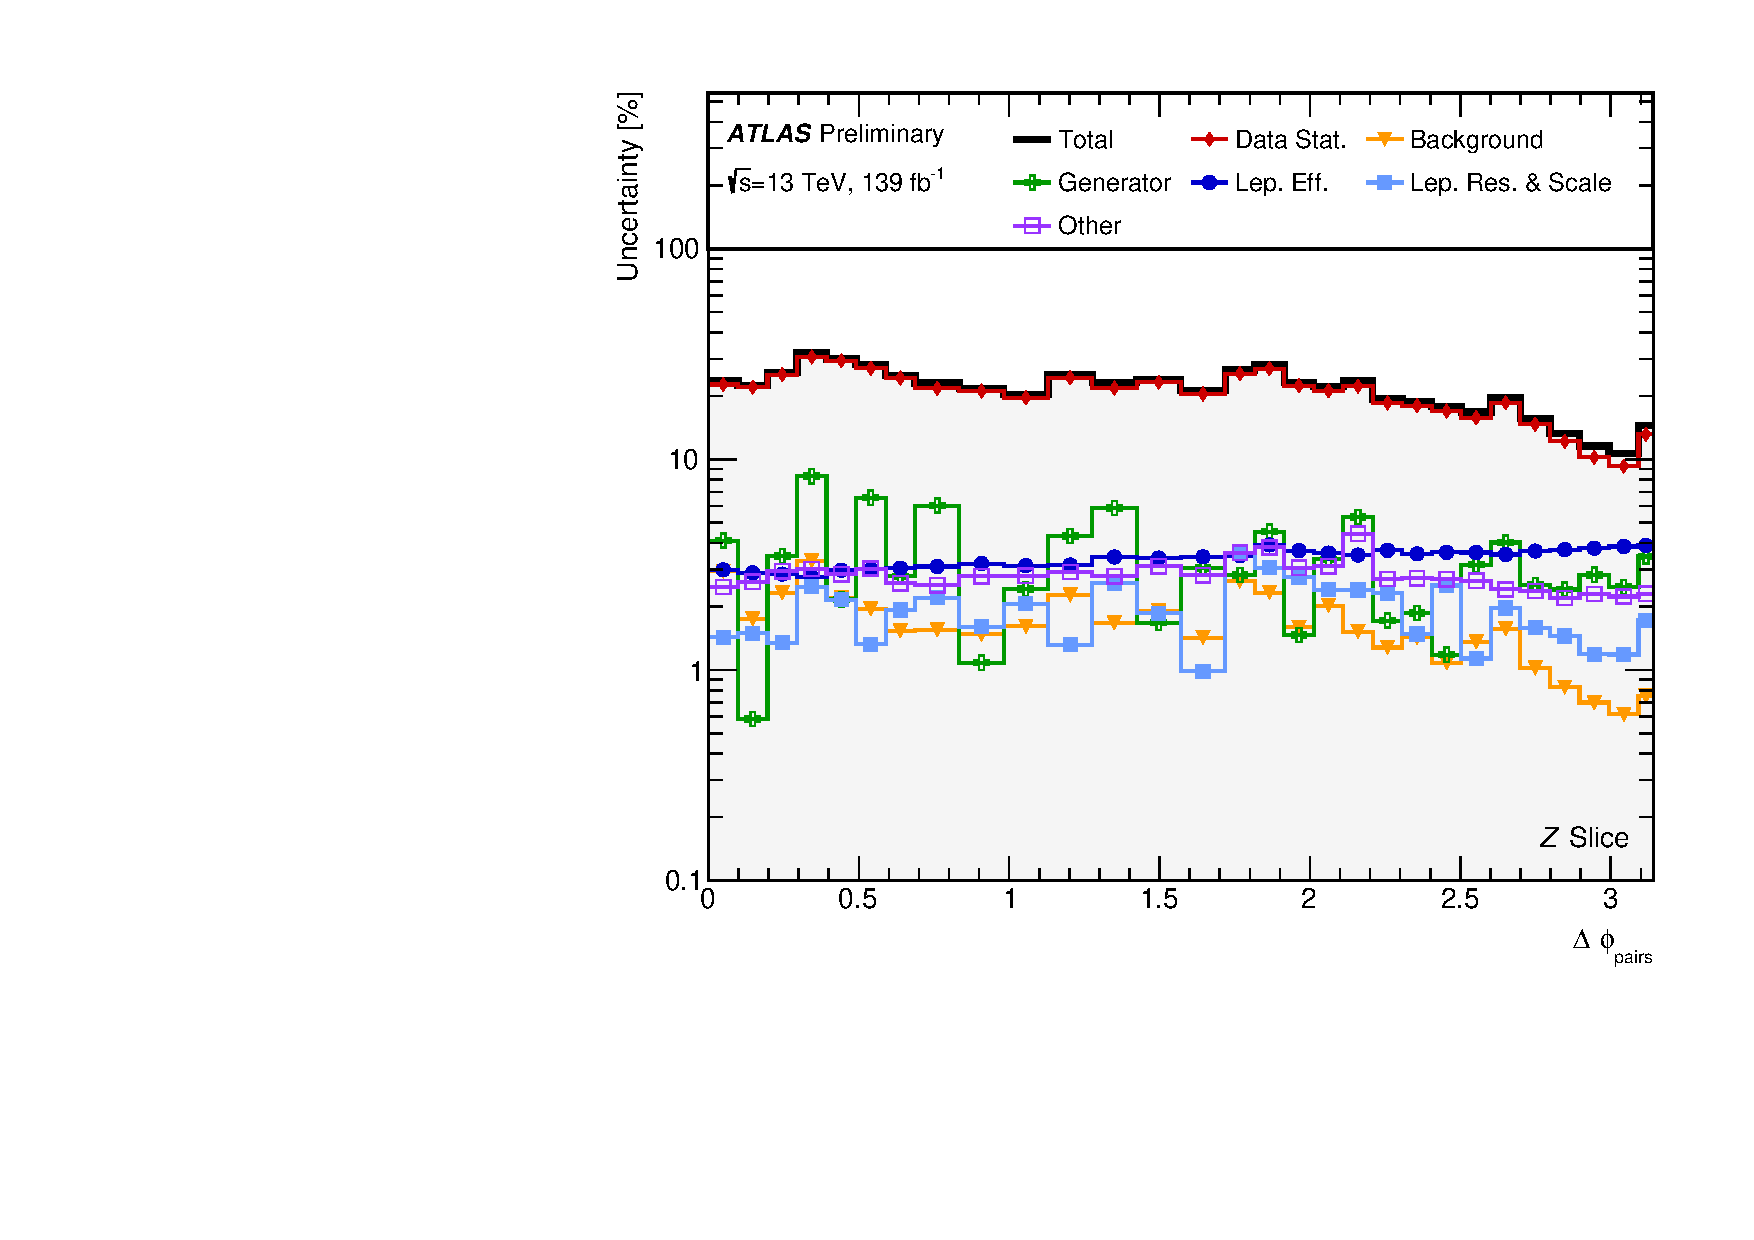
\includegraphics[width = 0.95\textwidth]{Figures/m4l/Systematics/Unfolded/UnfoldedSys_dPhiPairs_vs_M4l_Stack_Paper0.pdf}\end{subfigure}
    \begin{subfigure}{.49\textwidth}\centering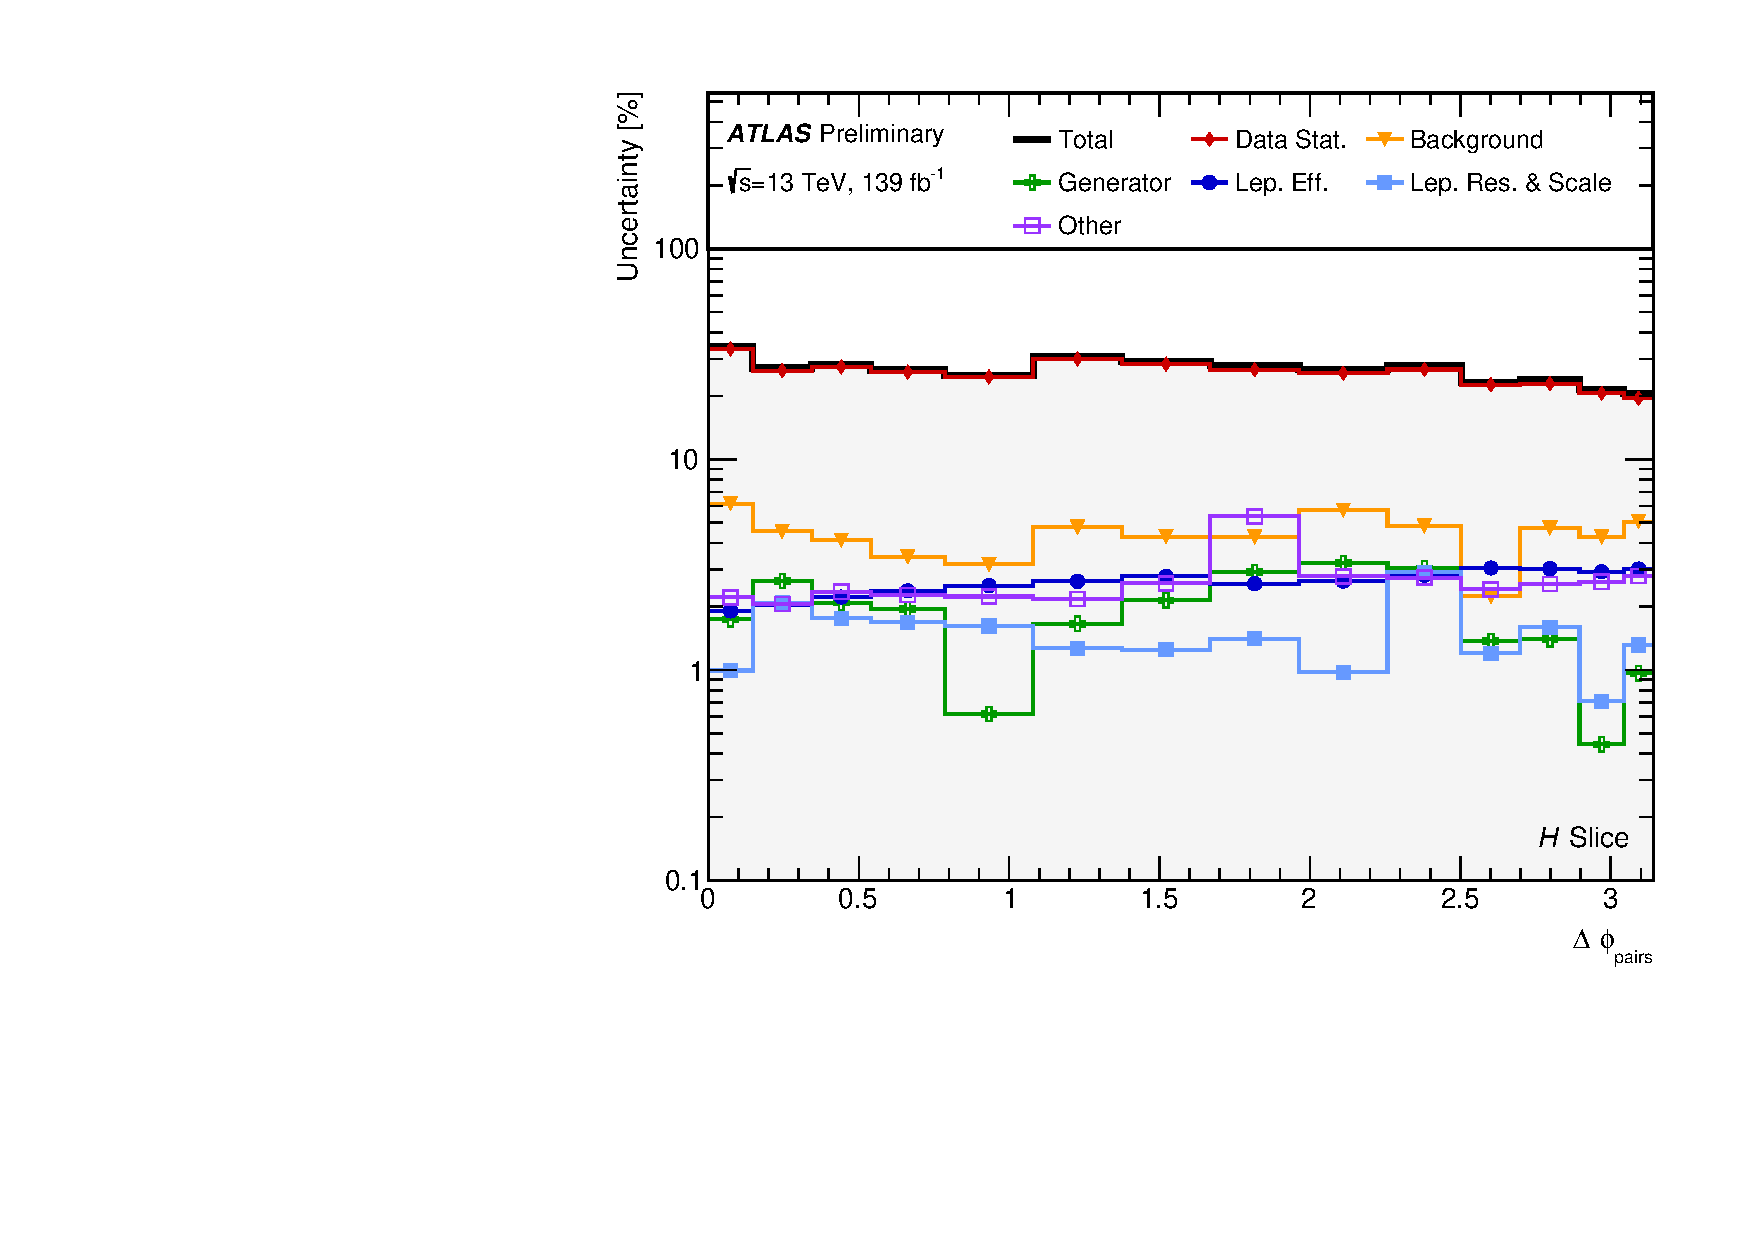
\includegraphics[width = 0.95\textwidth]{Figures/m4l/Systematics/Unfolded/UnfoldedSys_dPhiPairs_vs_M4l_Stack_Paper1.pdf}\end{subfigure}
    \begin{subfigure}{.49\textwidth}\centering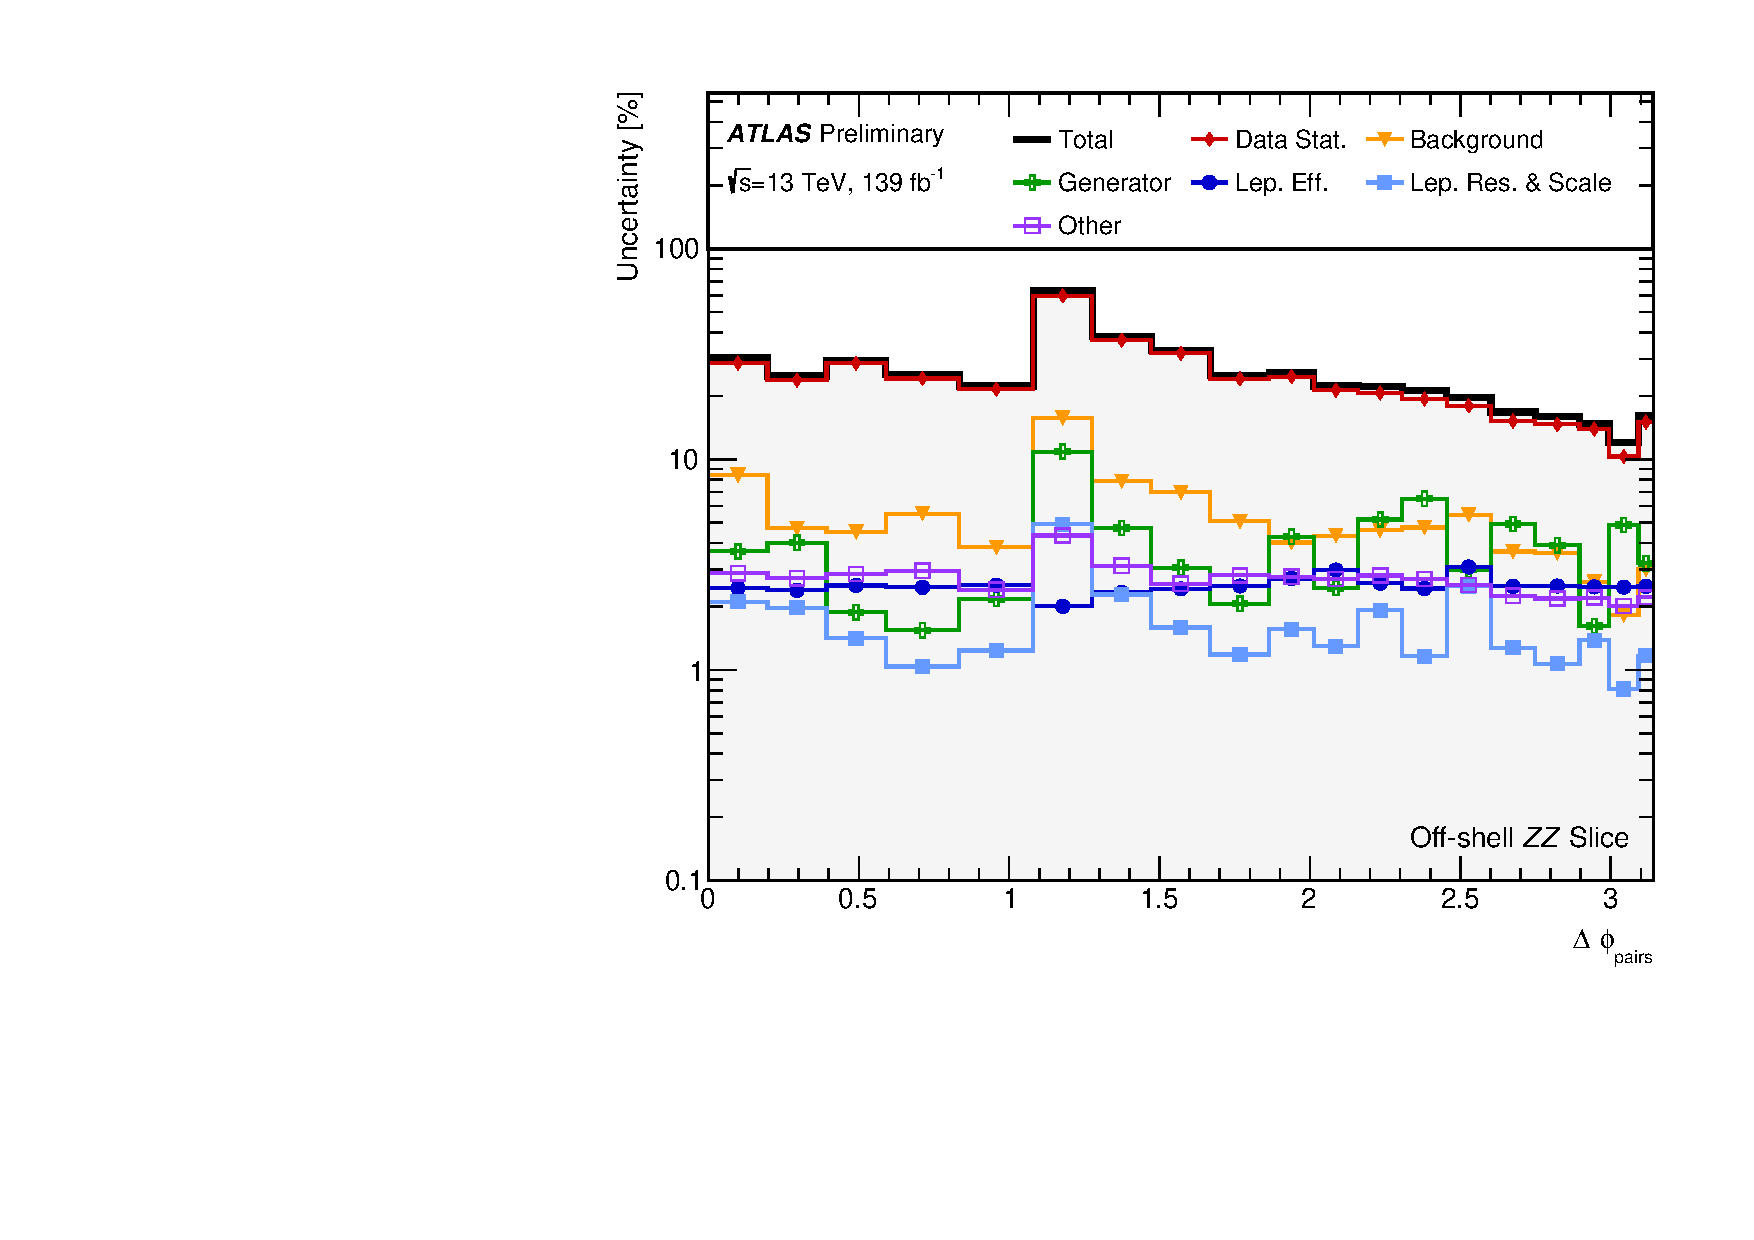
\includegraphics[width = 0.95\textwidth]{Figures/m4l/Systematics/Unfolded/UnfoldedSys_dPhiPairs_vs_M4l_Stack_Paper2.pdf}\end{subfigure}
    \begin{subfigure}{.49\textwidth}\centering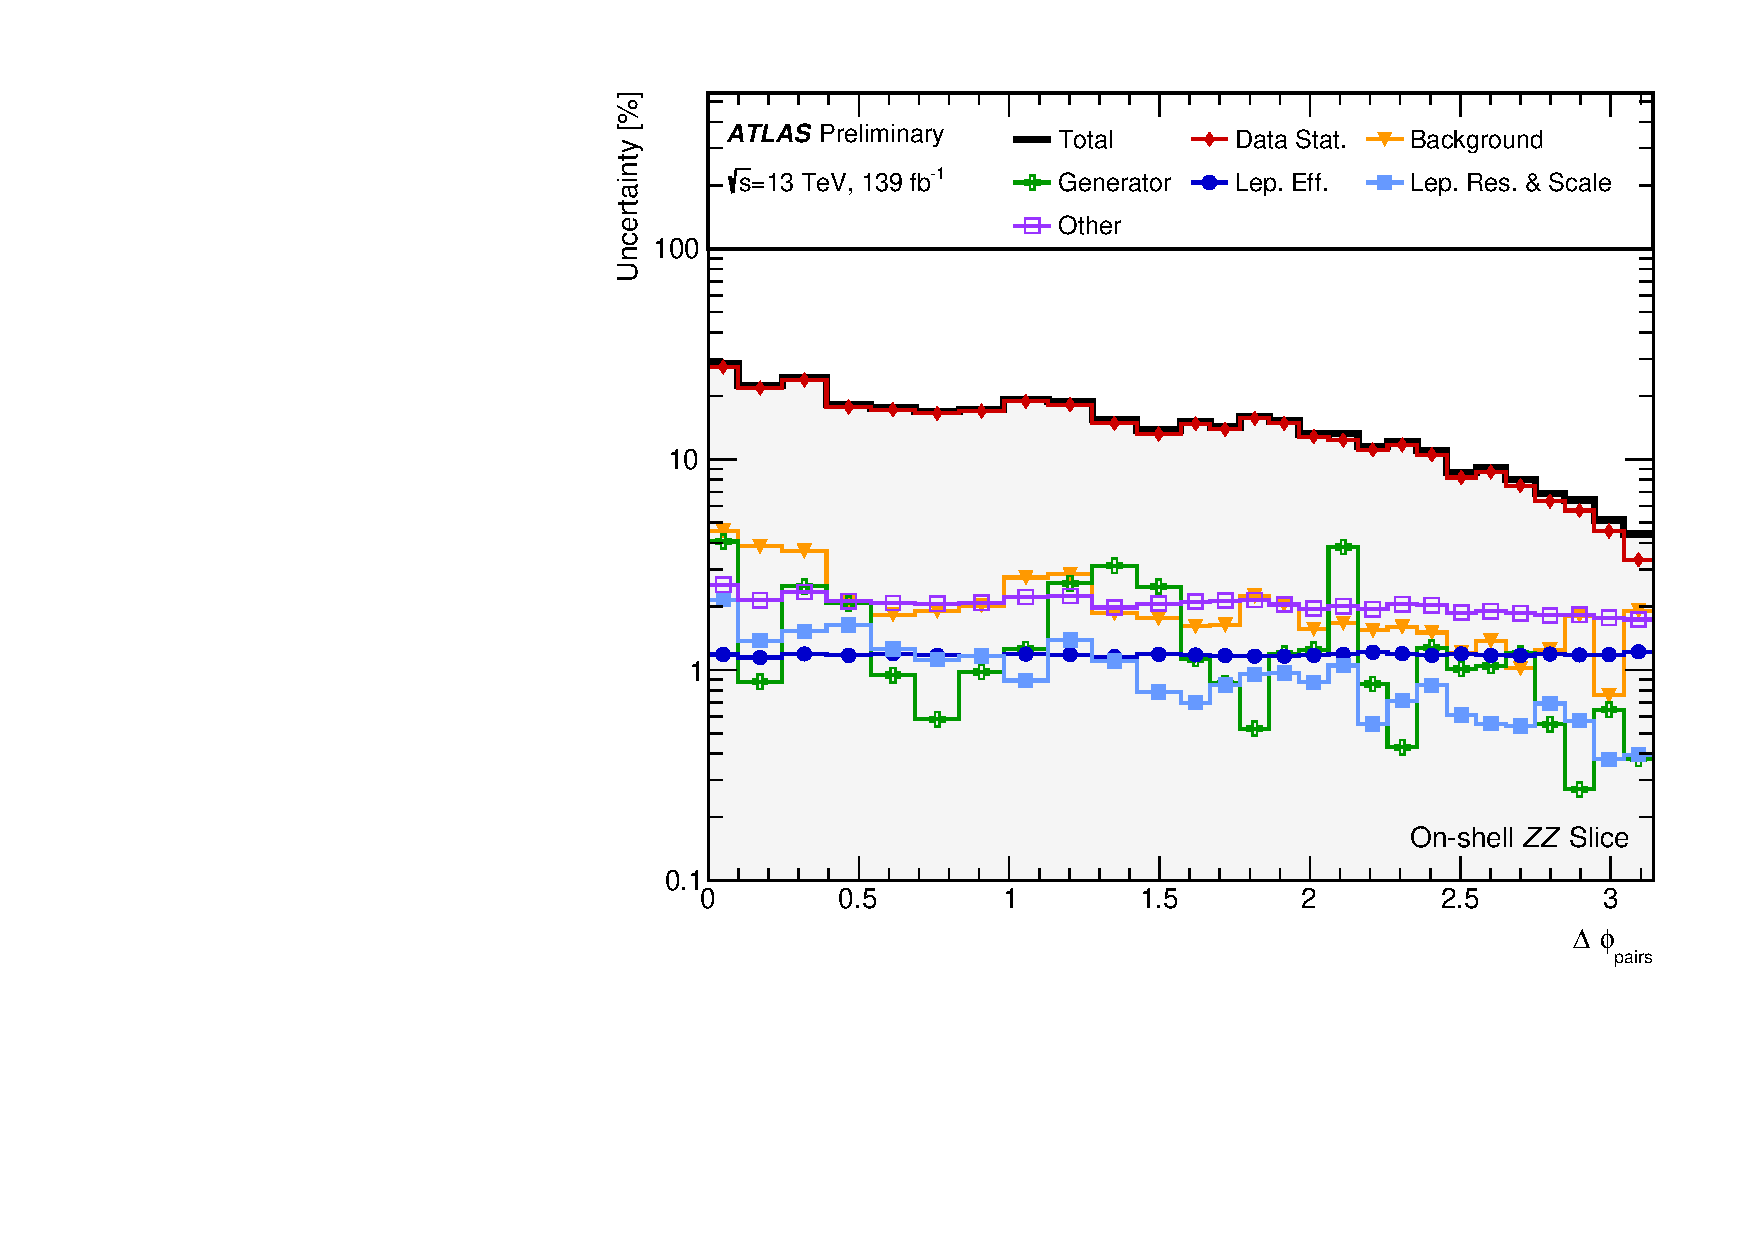
\includegraphics[width = 0.95\textwidth]{Figures/m4l/Systematics/Unfolded/UnfoldedSys_dPhiPairs_vs_M4l_Stack_Paper3.pdf}\end{subfigure}
    \caption{Unfolded systematics versus $\dPhiPairs$, in slices of $\mFourL$.}
\end{figure}

\begin{figure}[hp]
    \centering
    \begin{subfigure}{.49\textwidth}\centering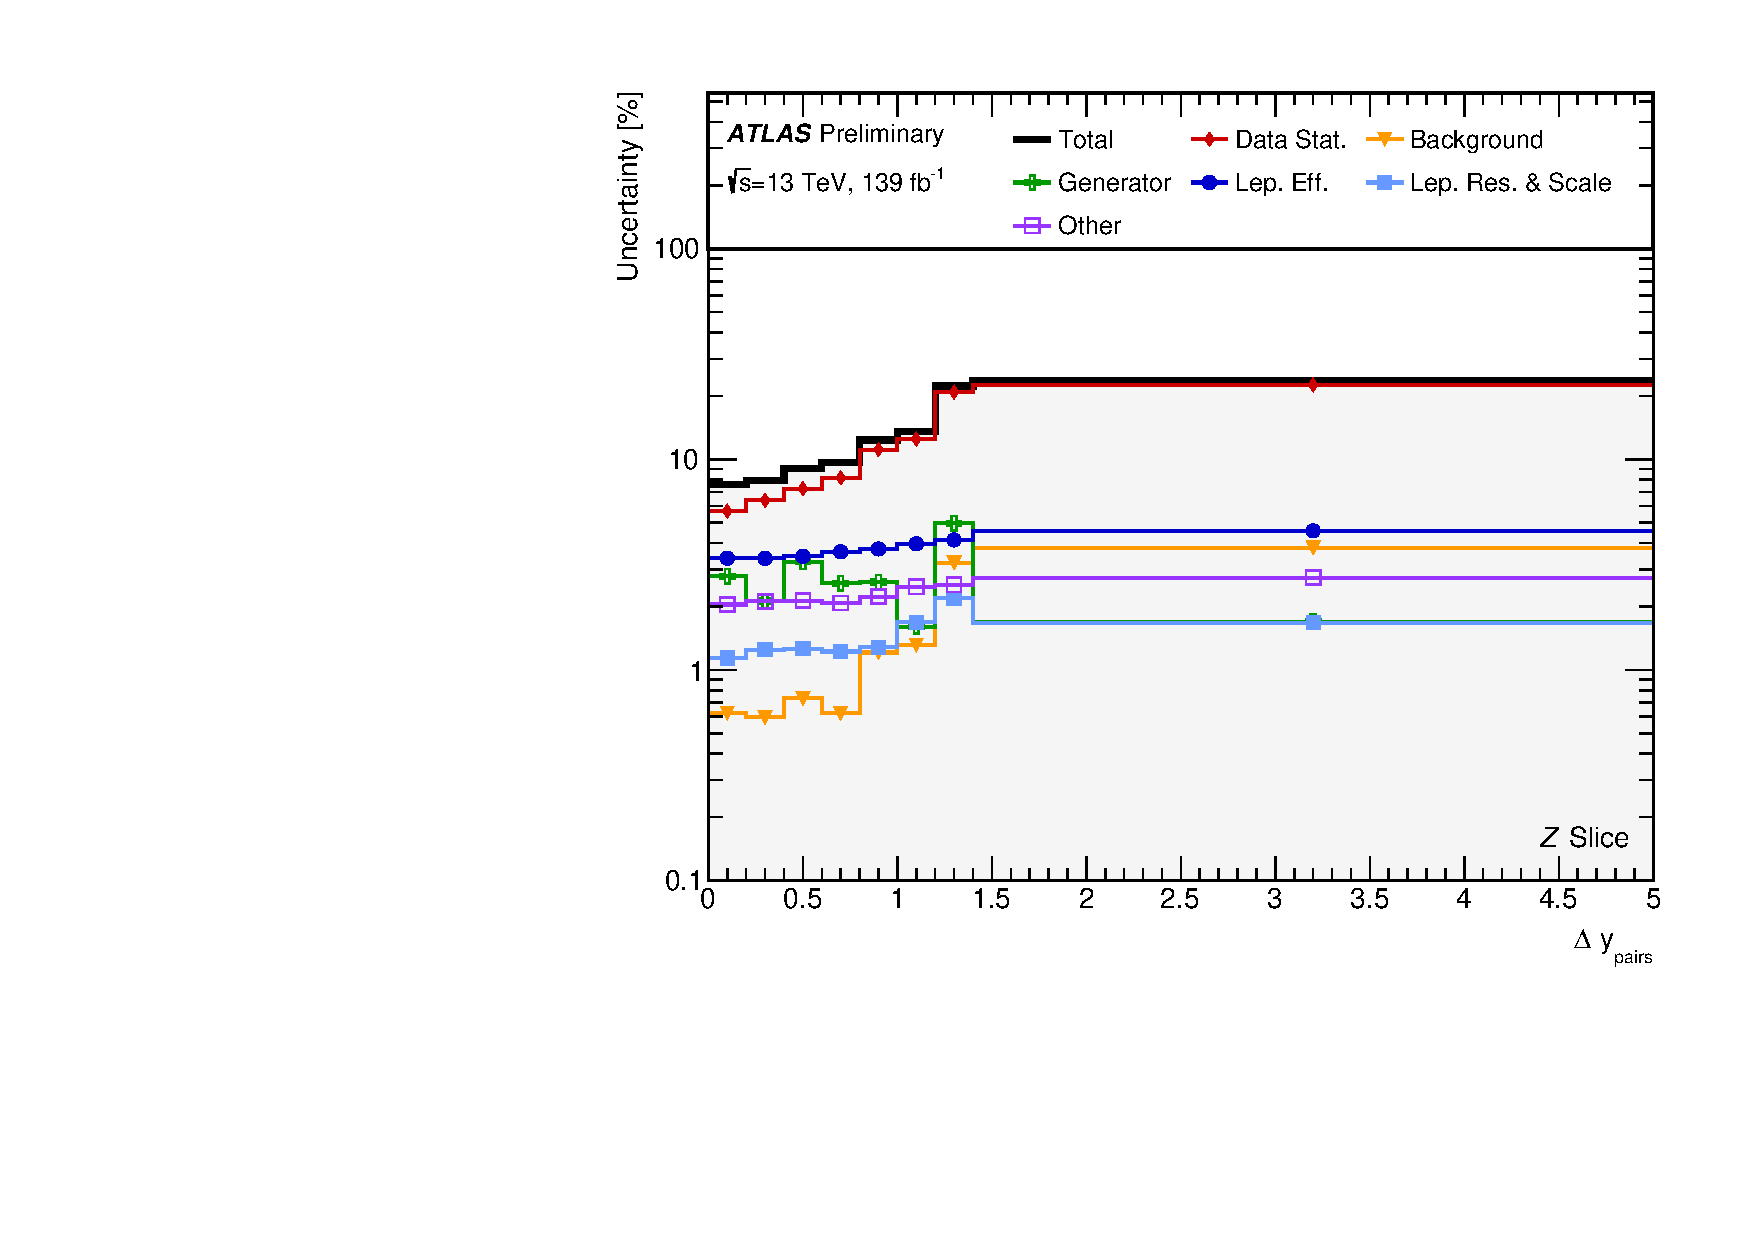
\includegraphics[width = 0.95\textwidth]{Figures/m4l/Systematics/Unfolded/UnfoldedSys_dYpairs_vs_M4l_Stack_Paper0.pdf}\end{subfigure}
    \begin{subfigure}{.49\textwidth}\centering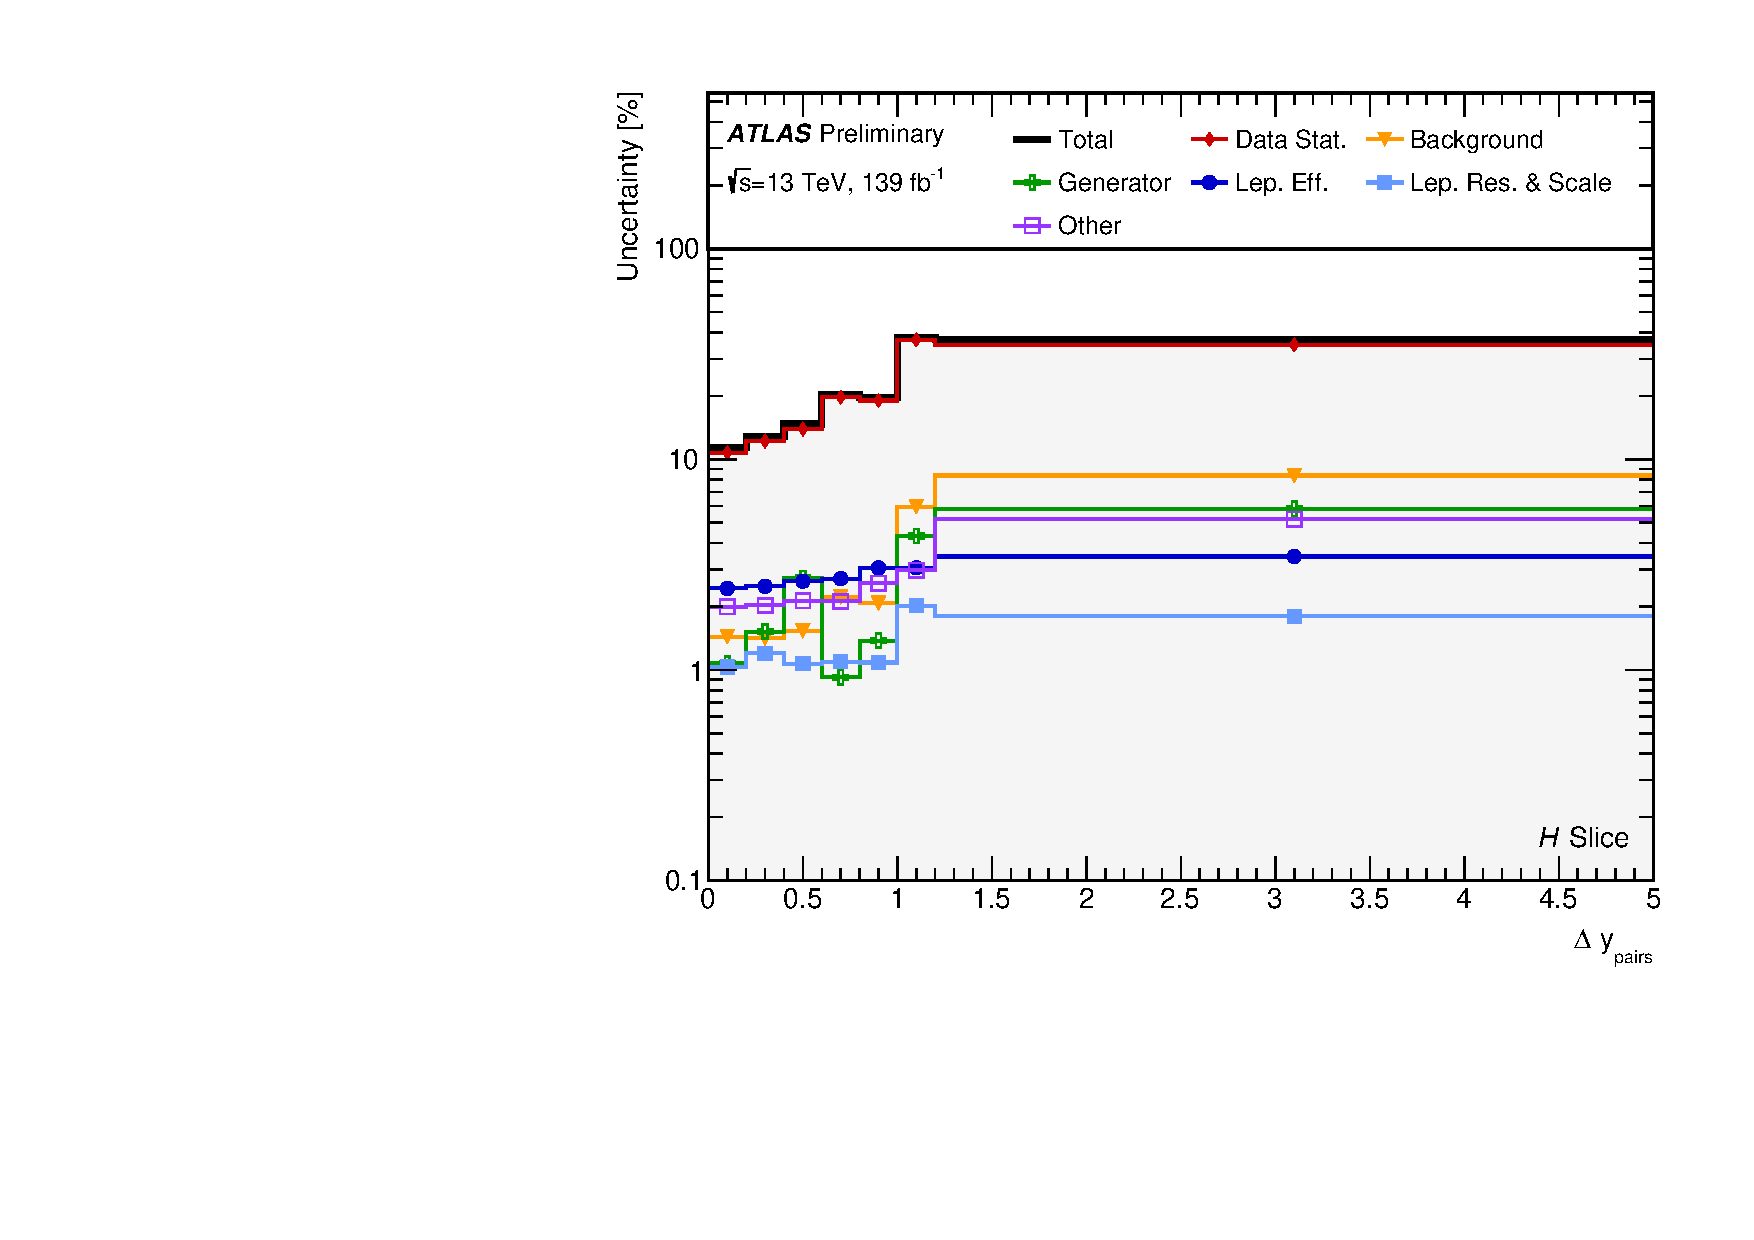
\includegraphics[width = 0.95\textwidth]{Figures/m4l/Systematics/Unfolded/UnfoldedSys_dYpairs_vs_M4l_Stack_Paper1.pdf}\end{subfigure}
    \begin{subfigure}{.49\textwidth}\centering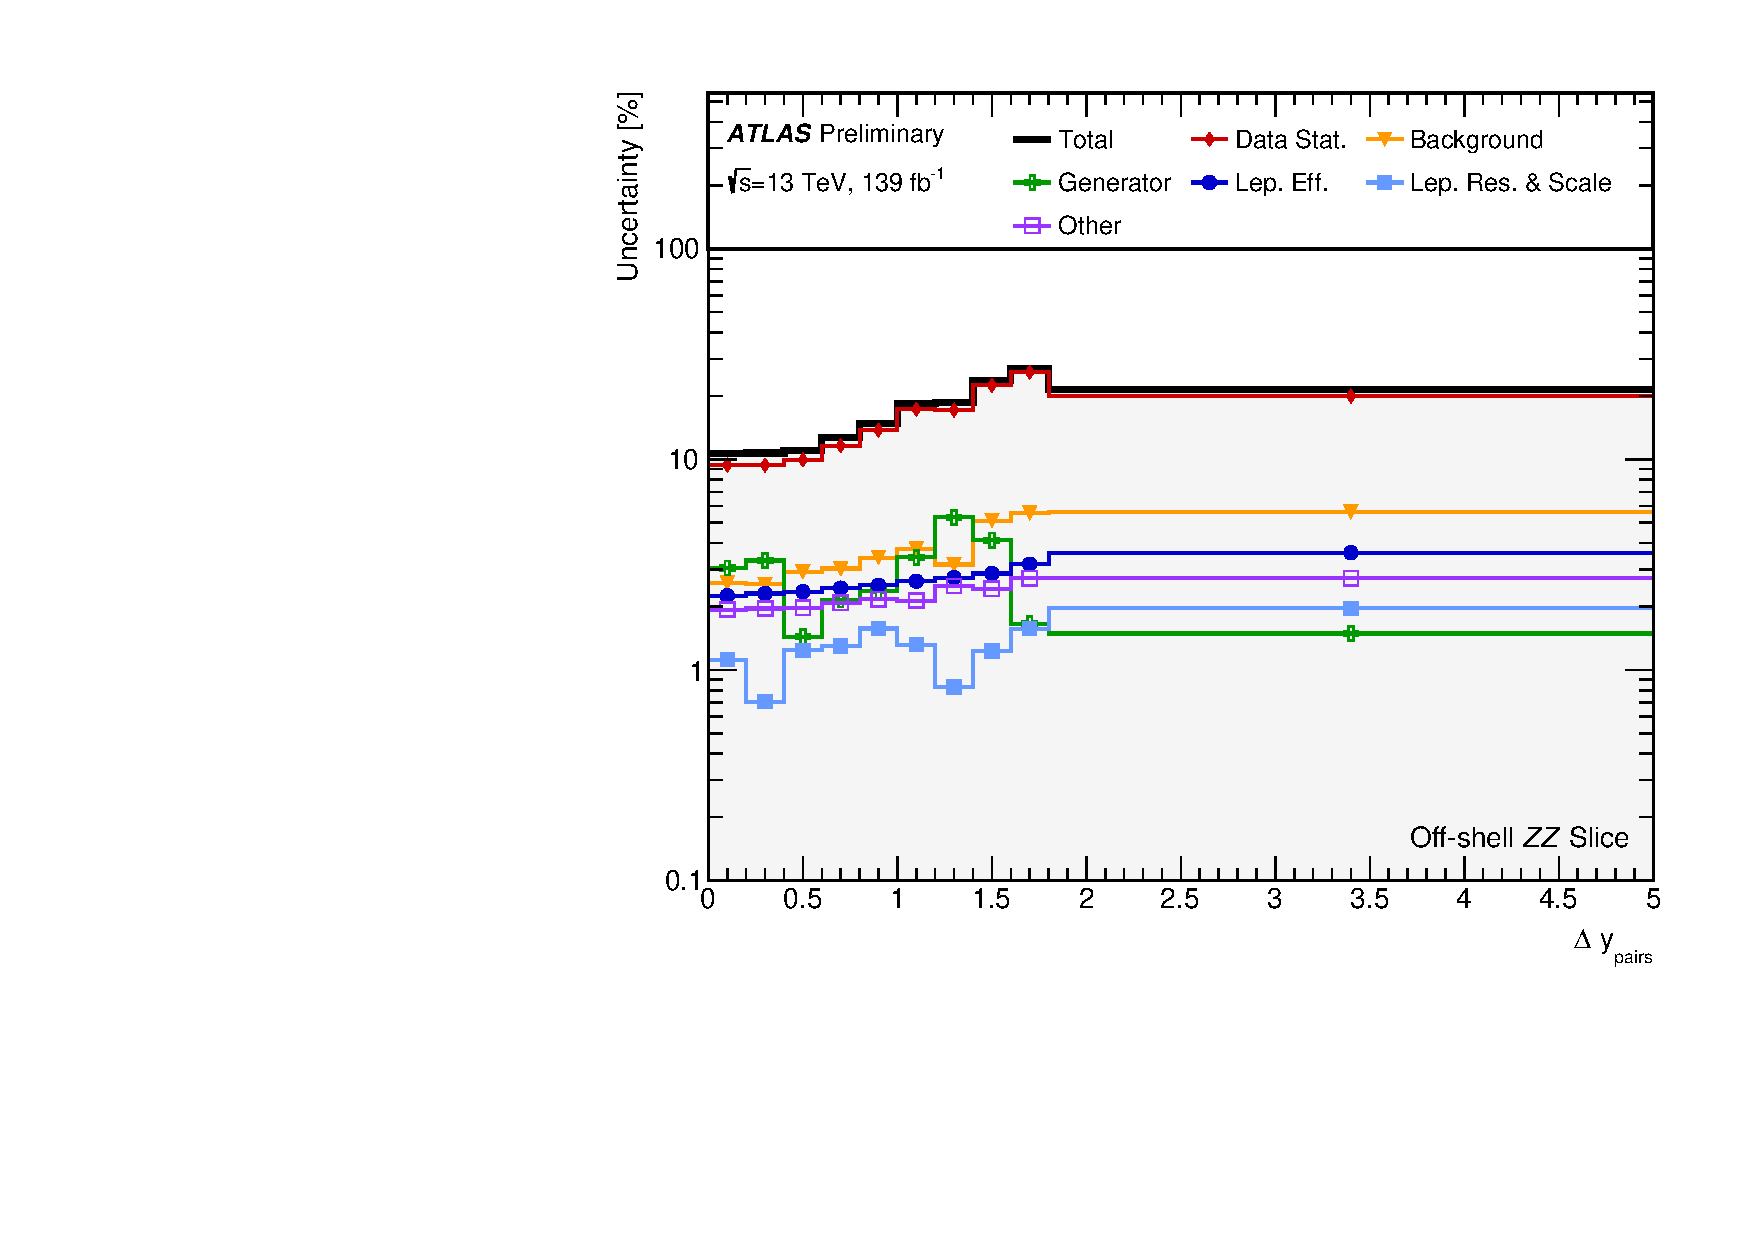
\includegraphics[width = 0.95\textwidth]{Figures/m4l/Systematics/Unfolded/UnfoldedSys_dYpairs_vs_M4l_Stack_Paper2.pdf}\end{subfigure}
    \begin{subfigure}{.49\textwidth}\centering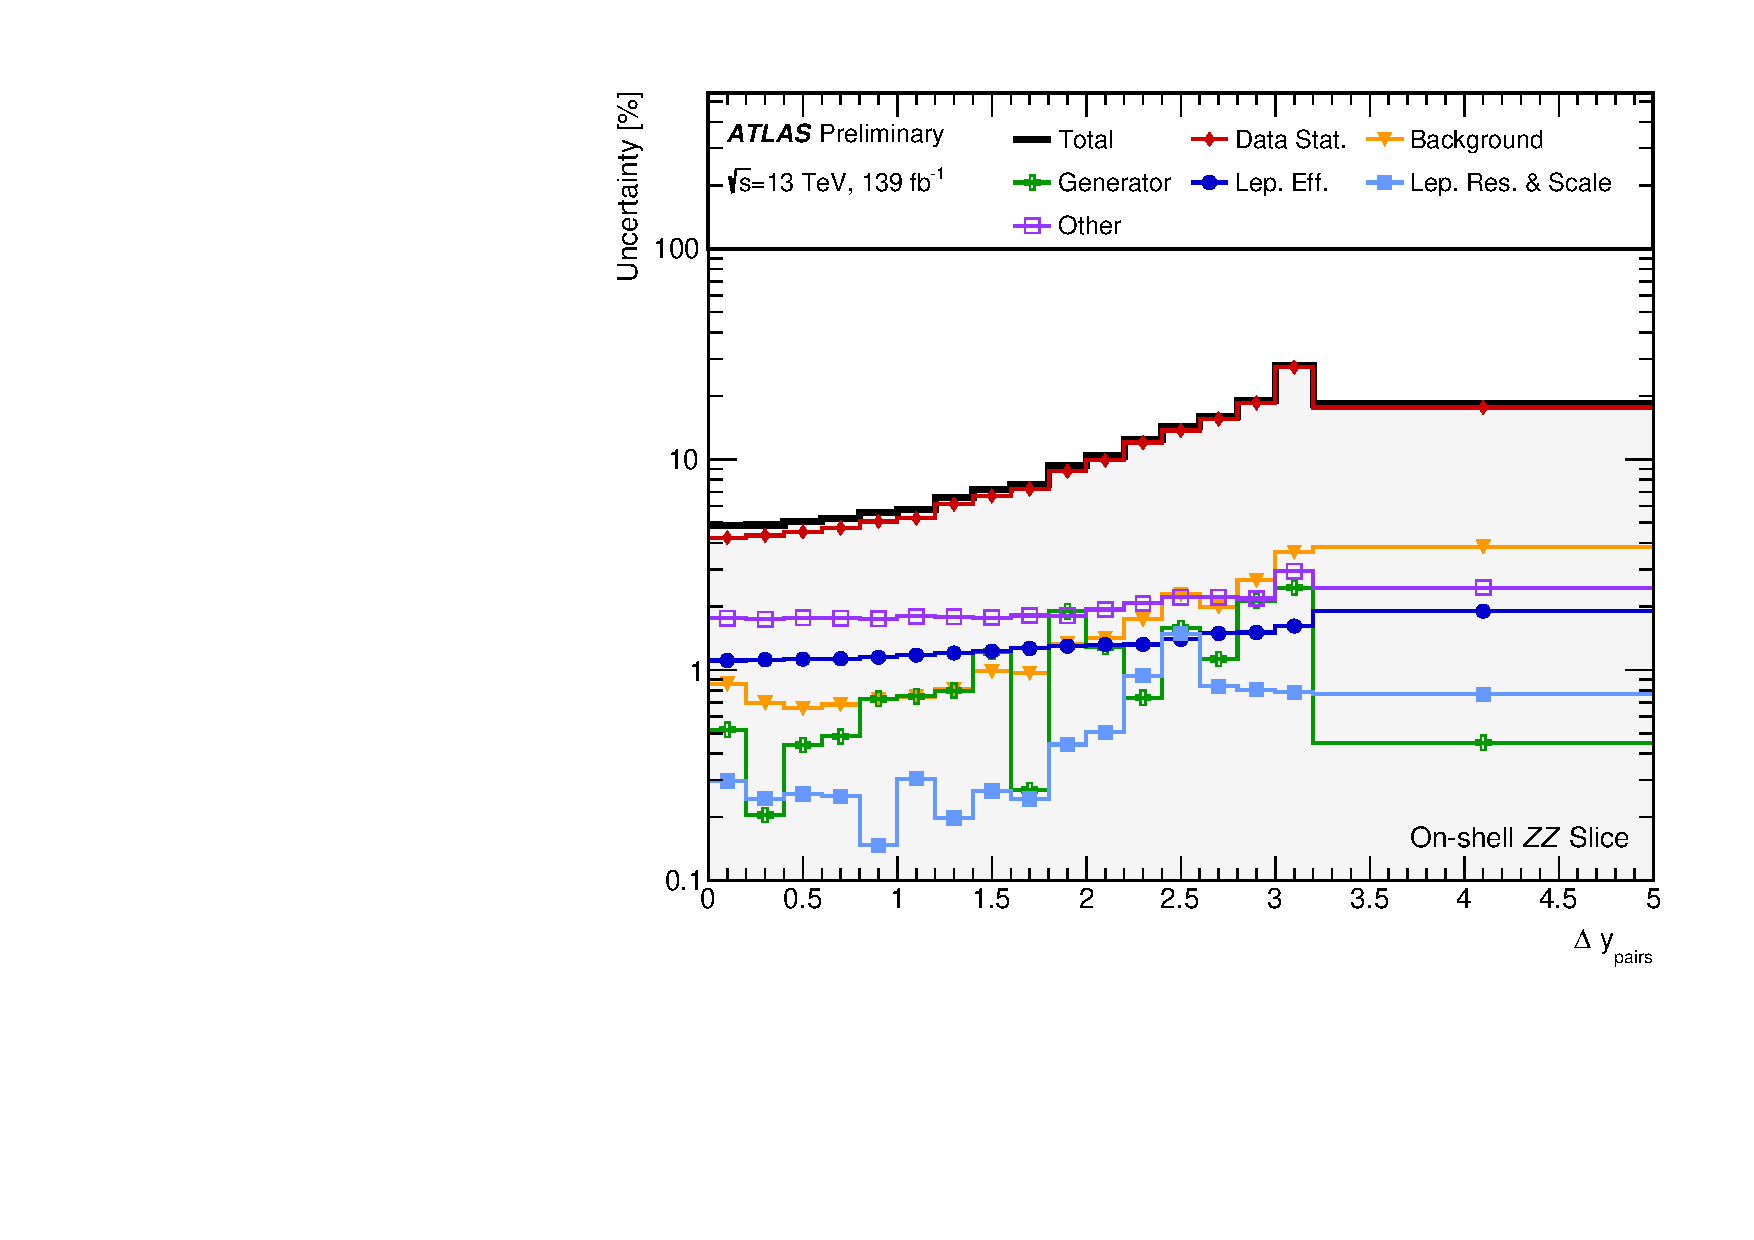
\includegraphics[width = 0.95\textwidth]{Figures/m4l/Systematics/Unfolded/UnfoldedSys_dYpairs_vs_M4l_Stack_Paper3.pdf}\end{subfigure}
    \caption{Unfolded systematics versus $\dYPairs$, in slices of $\mFourL$.}
\end{figure}

\begin{figure}[hp]
    \centering
    \begin{subfigure}{.49\textwidth}\centering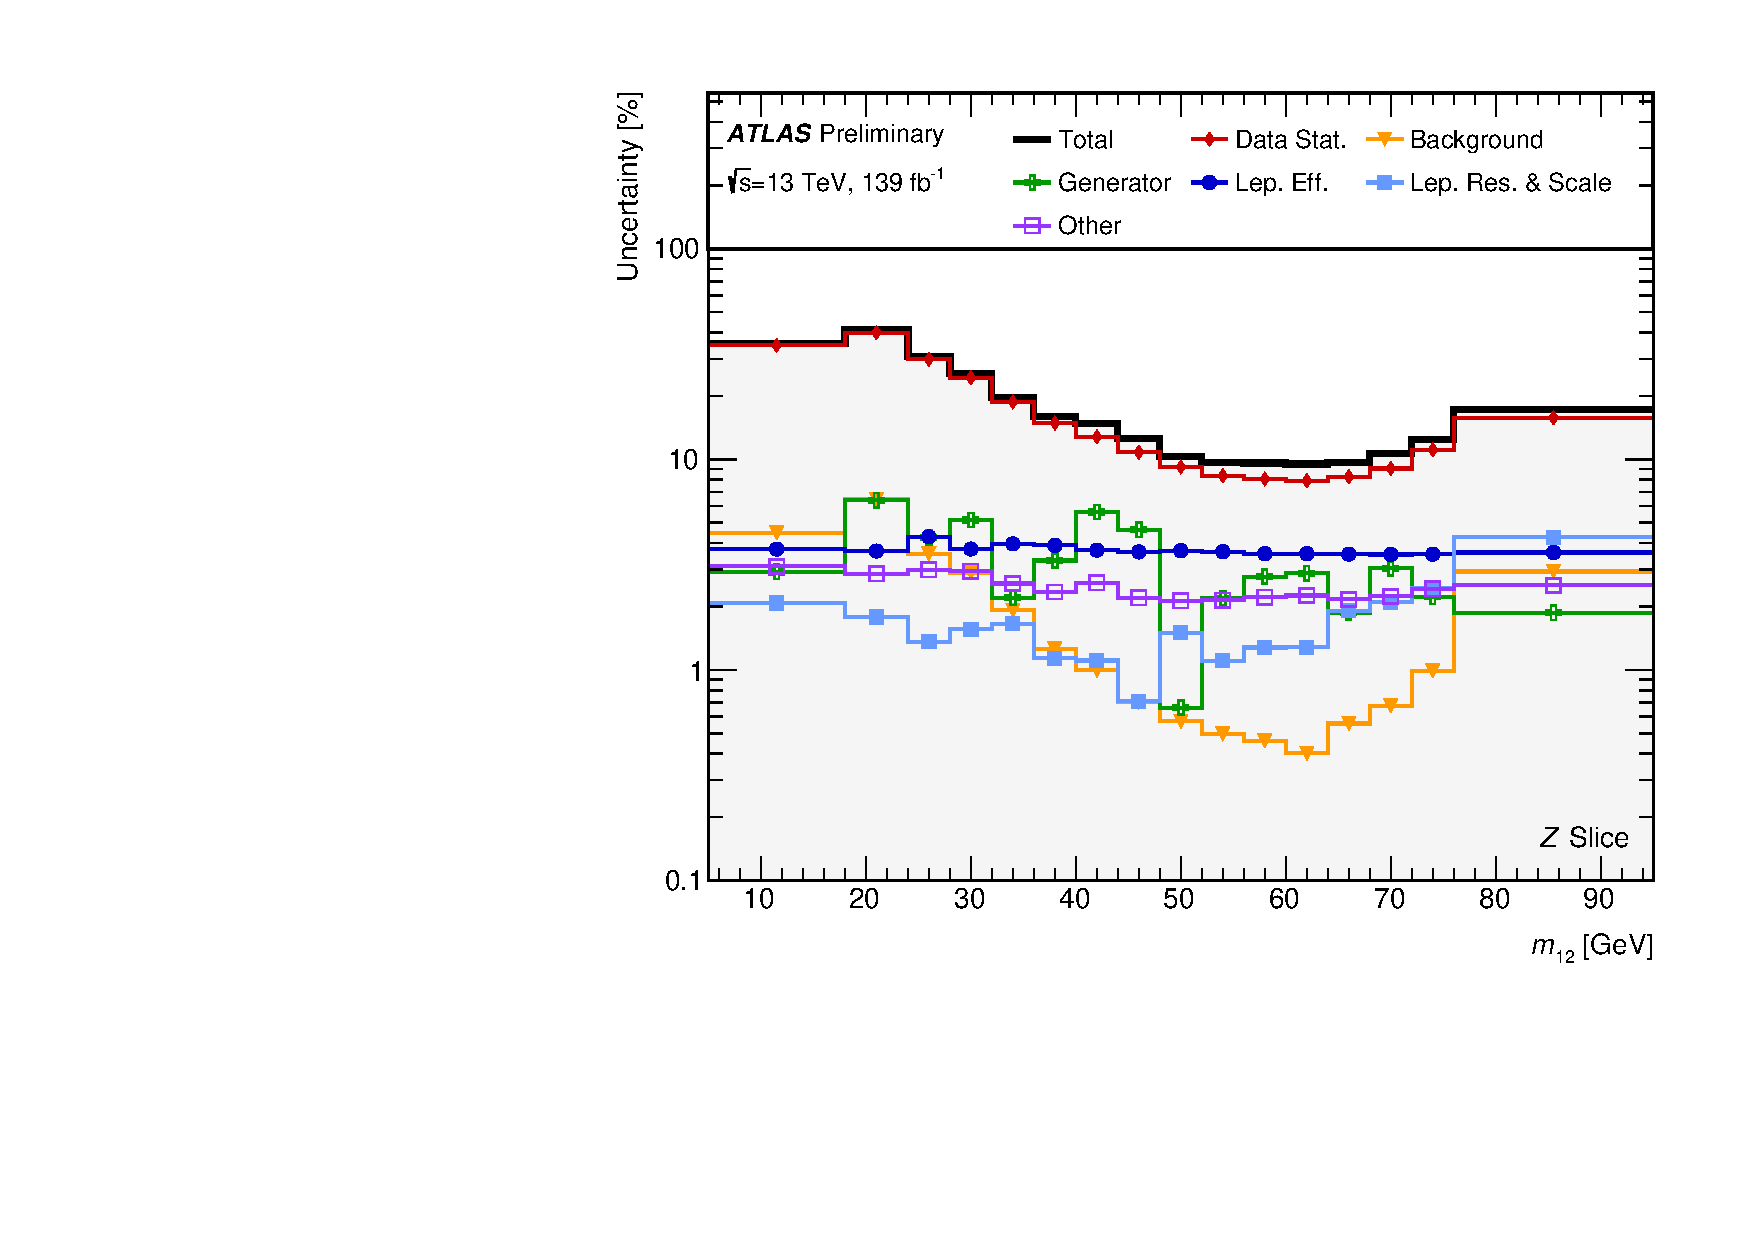
\includegraphics[width = 0.95\textwidth]{Figures/m4l/Systematics/Unfolded/UnfoldedSys_m12_vs_M4l_Stack_Paper0.pdf}\end{subfigure}
    \begin{subfigure}{.49\textwidth}\centering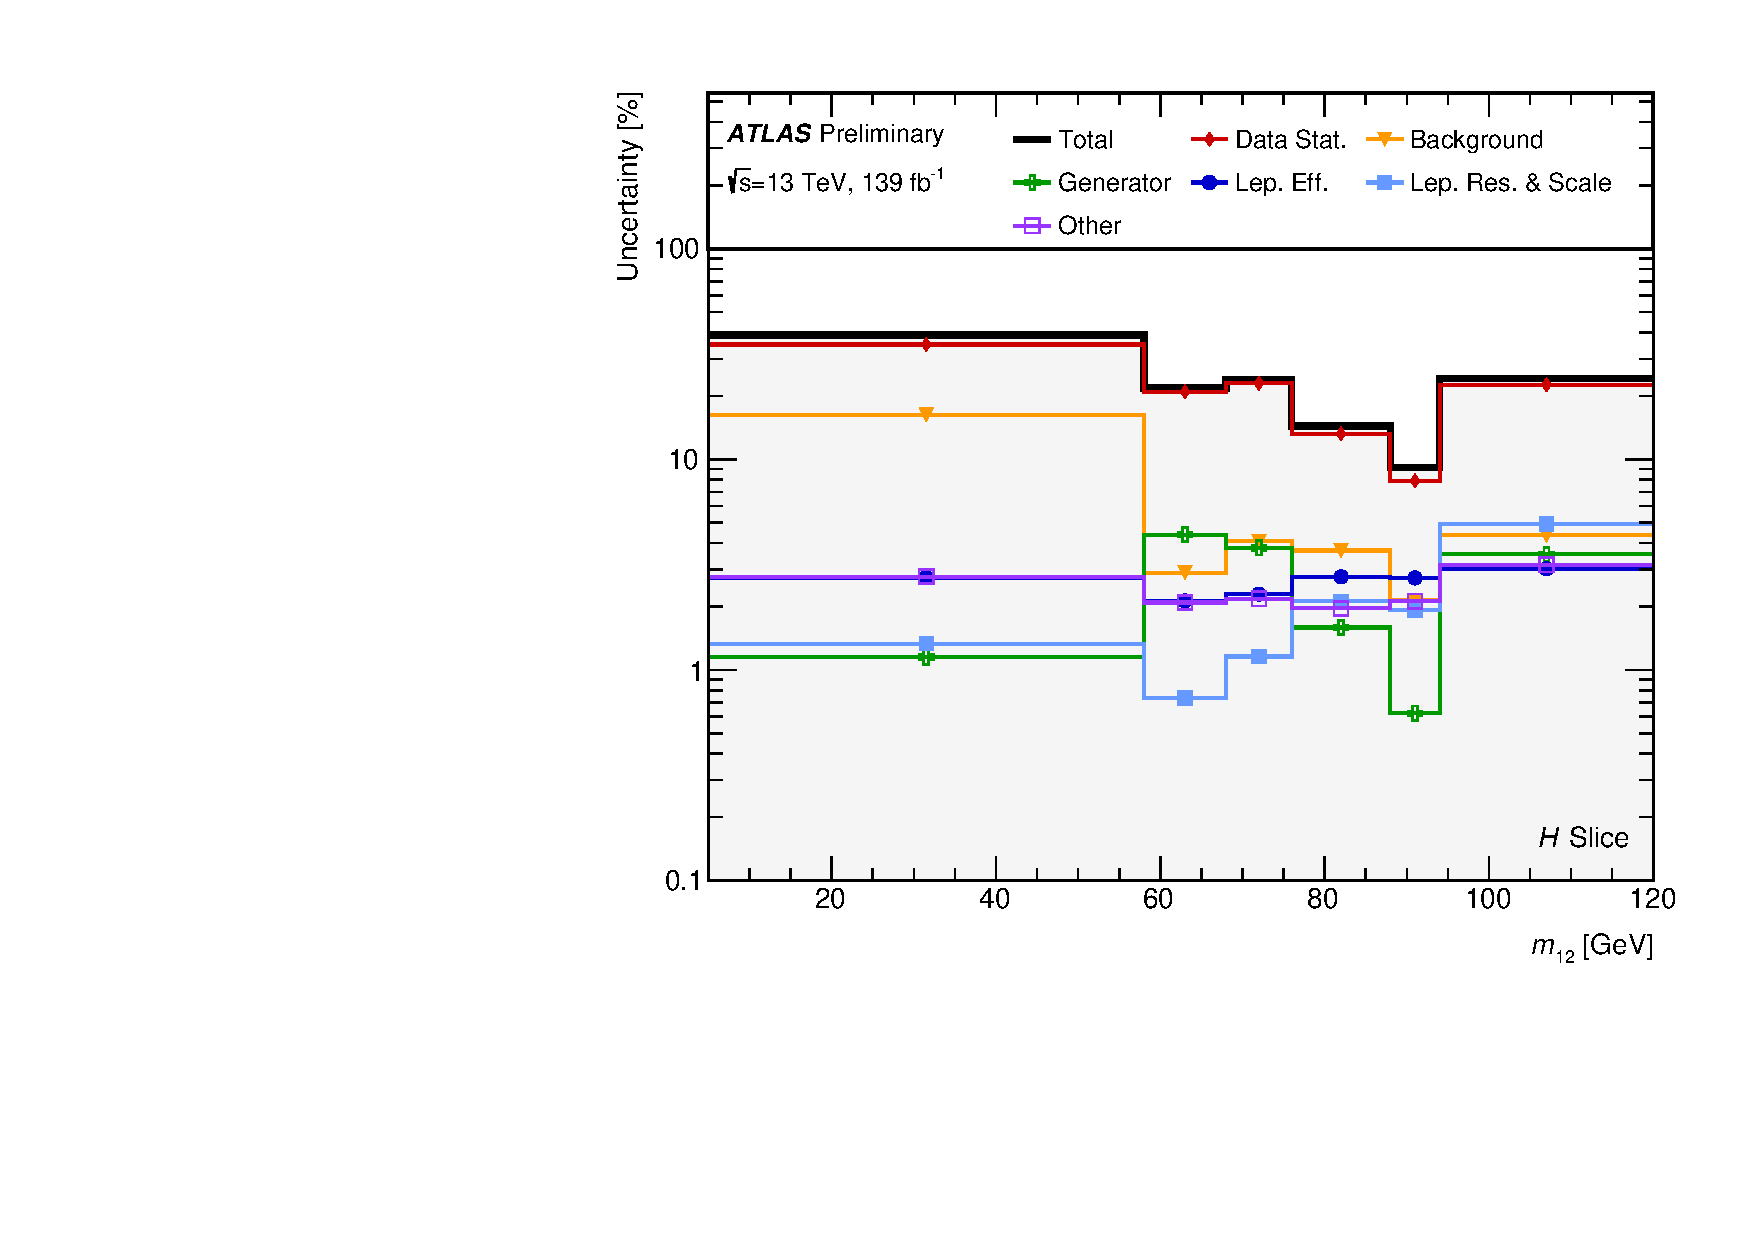
\includegraphics[width = 0.95\textwidth]{Figures/m4l/Systematics/Unfolded/UnfoldedSys_m12_vs_M4l_Stack_Paper1.pdf}\end{subfigure}
    \begin{subfigure}{.49\textwidth}\centering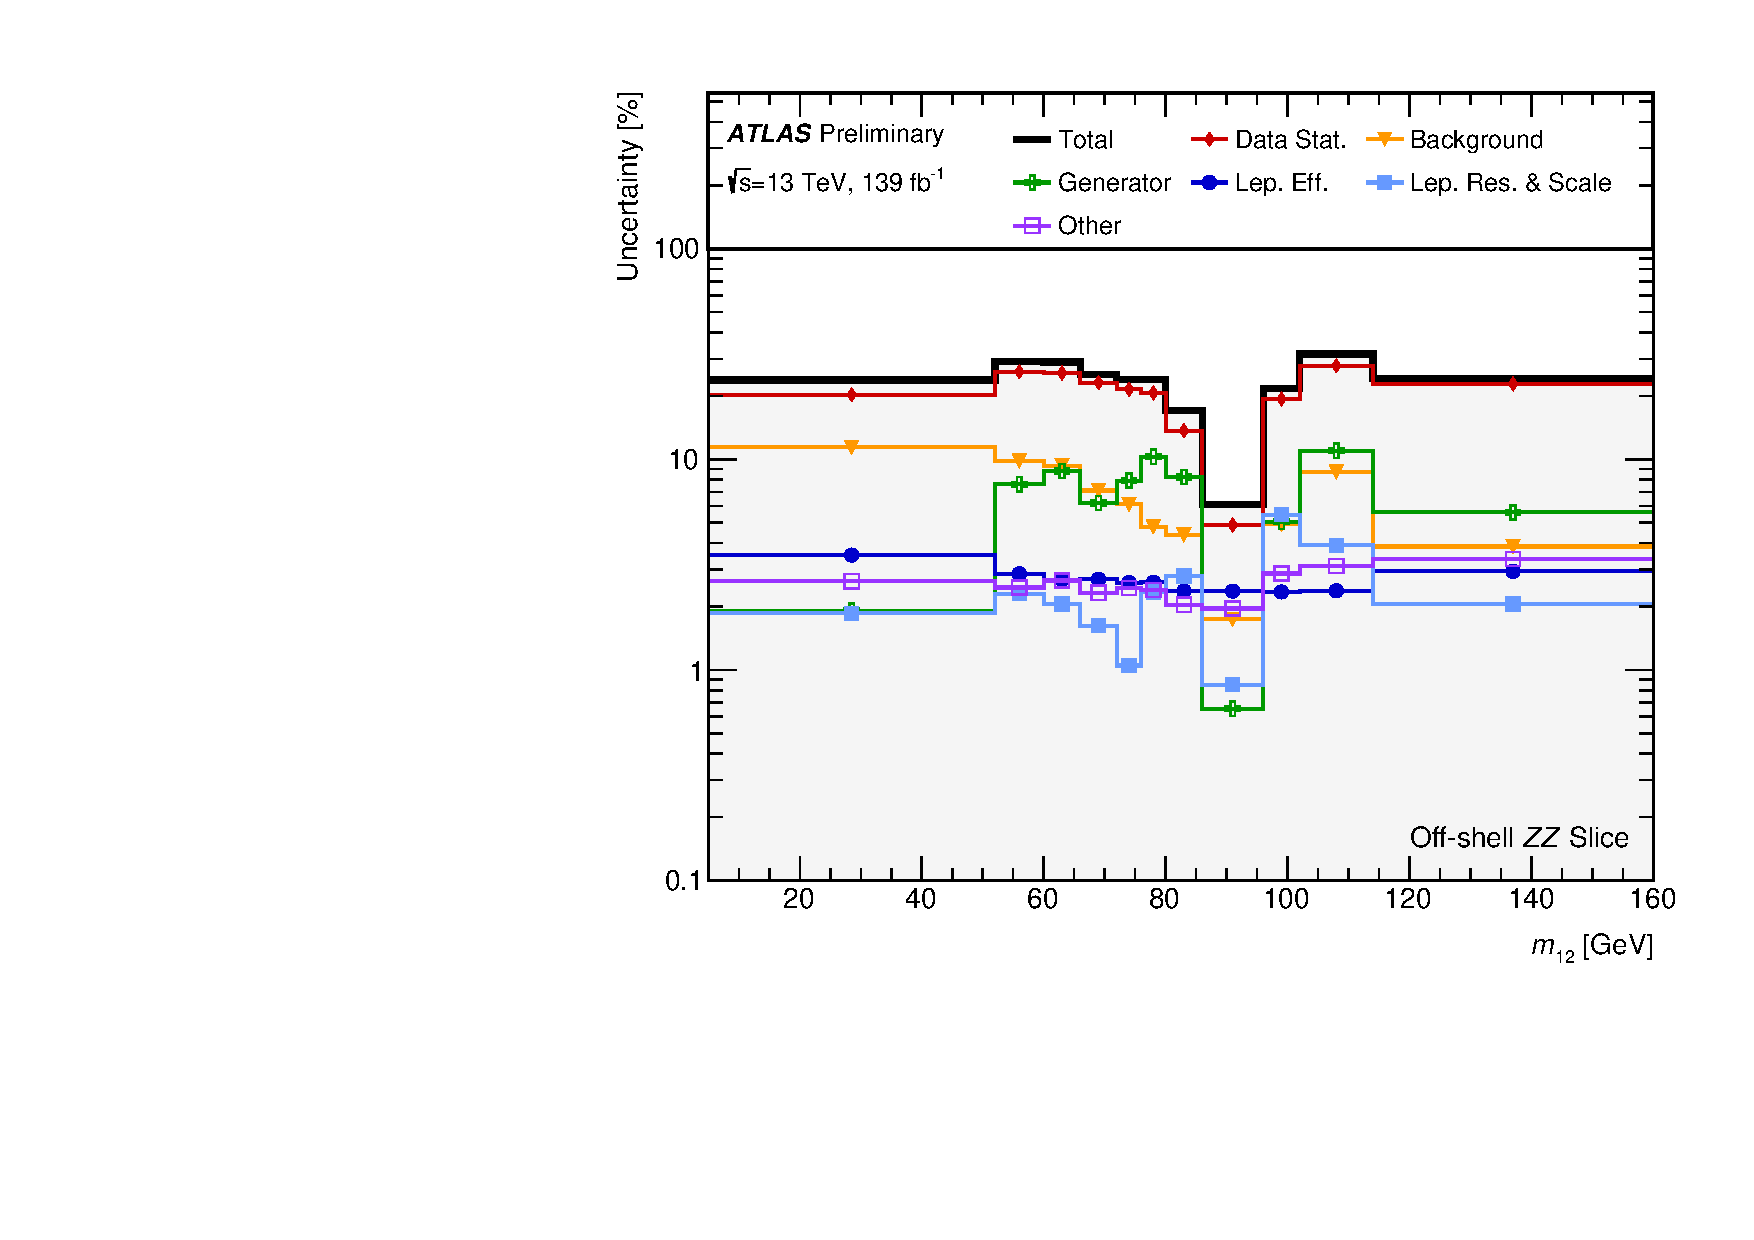
\includegraphics[width = 0.95\textwidth]{Figures/m4l/Systematics/Unfolded/UnfoldedSys_m12_vs_M4l_Stack_Paper2.pdf}\end{subfigure}
    \begin{subfigure}{.49\textwidth}\centering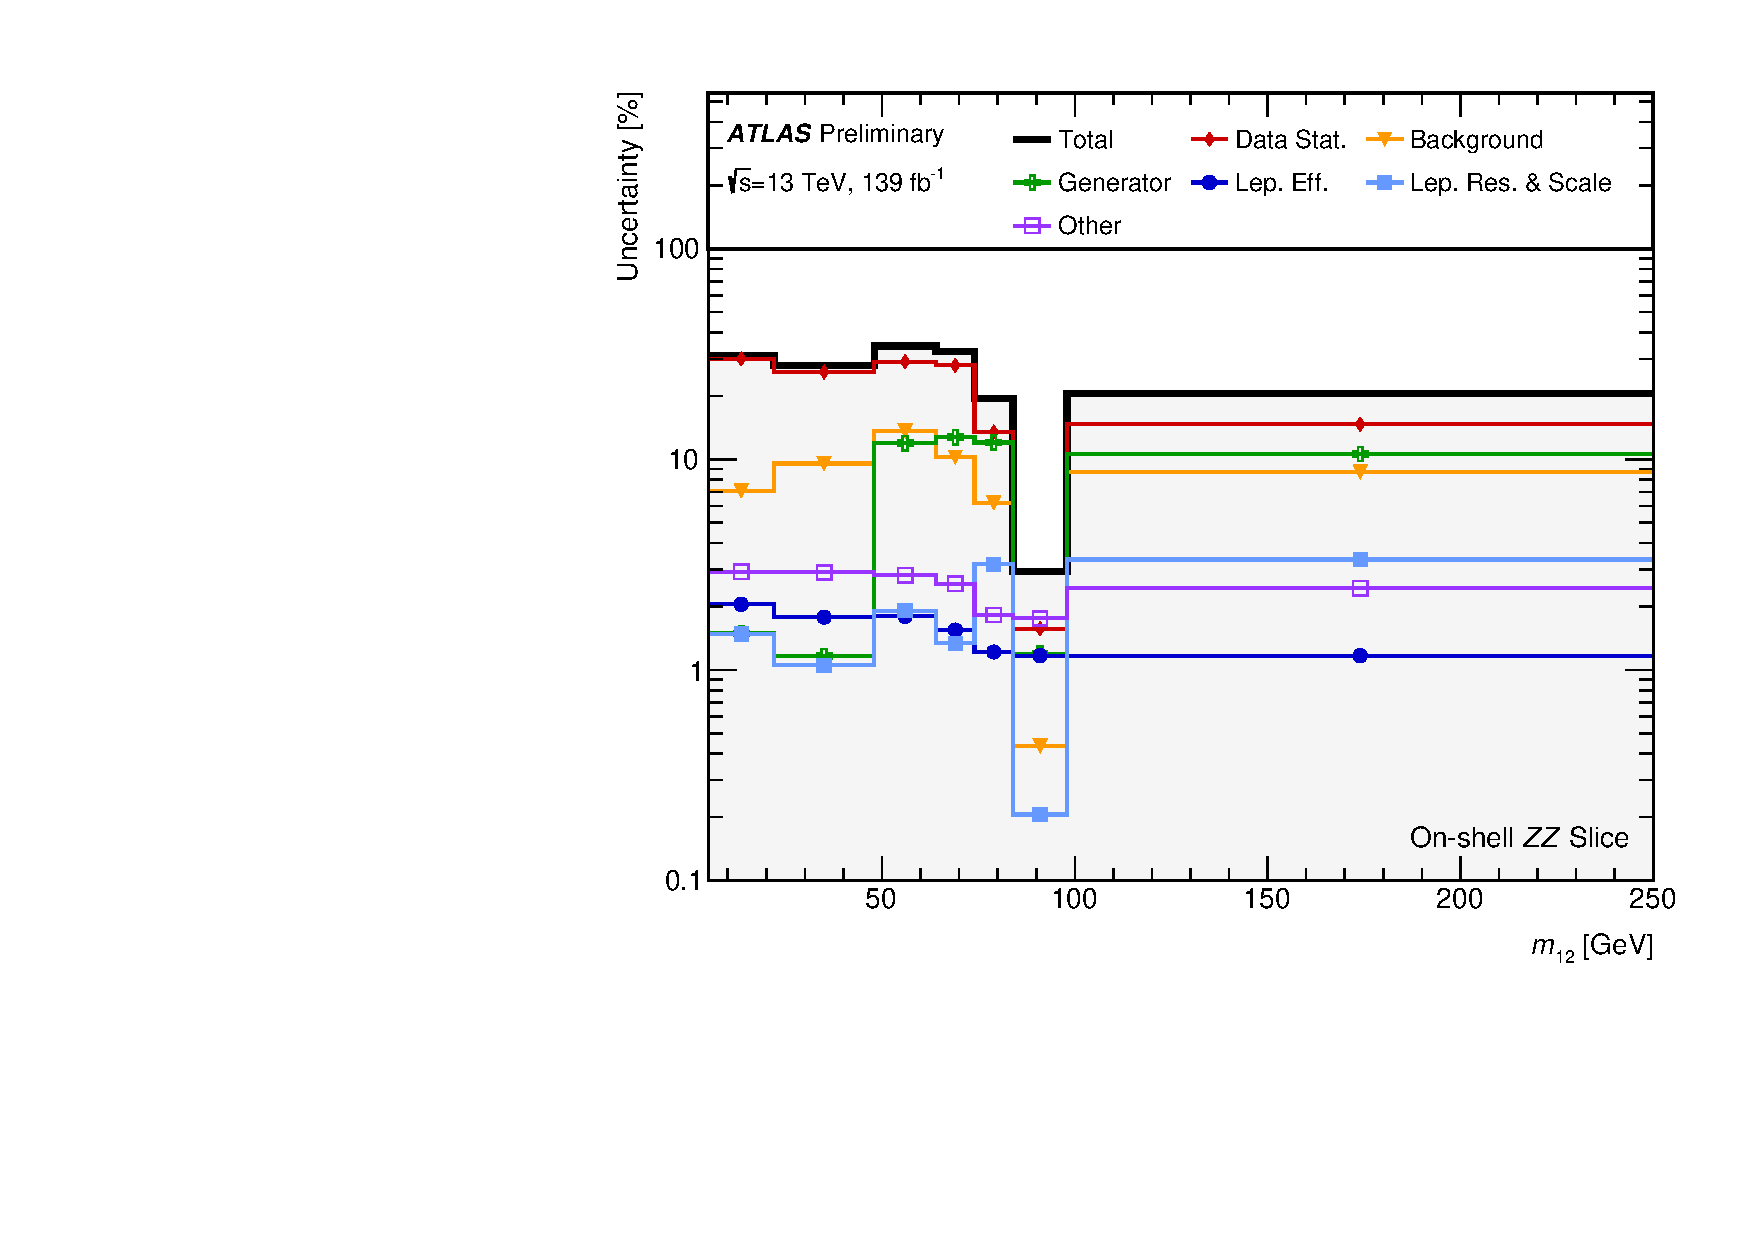
\includegraphics[width = 0.95\textwidth]{Figures/m4l/Systematics/Unfolded/UnfoldedSys_m12_vs_M4l_Stack_Paper3.pdf}\end{subfigure}
    \caption{Unfolded systematics versus $\mZOne$, in slices of $\mFourL$.}
\end{figure}

\begin{figure}[hp]
    \centering
    \begin{subfigure}{.49\textwidth}\centering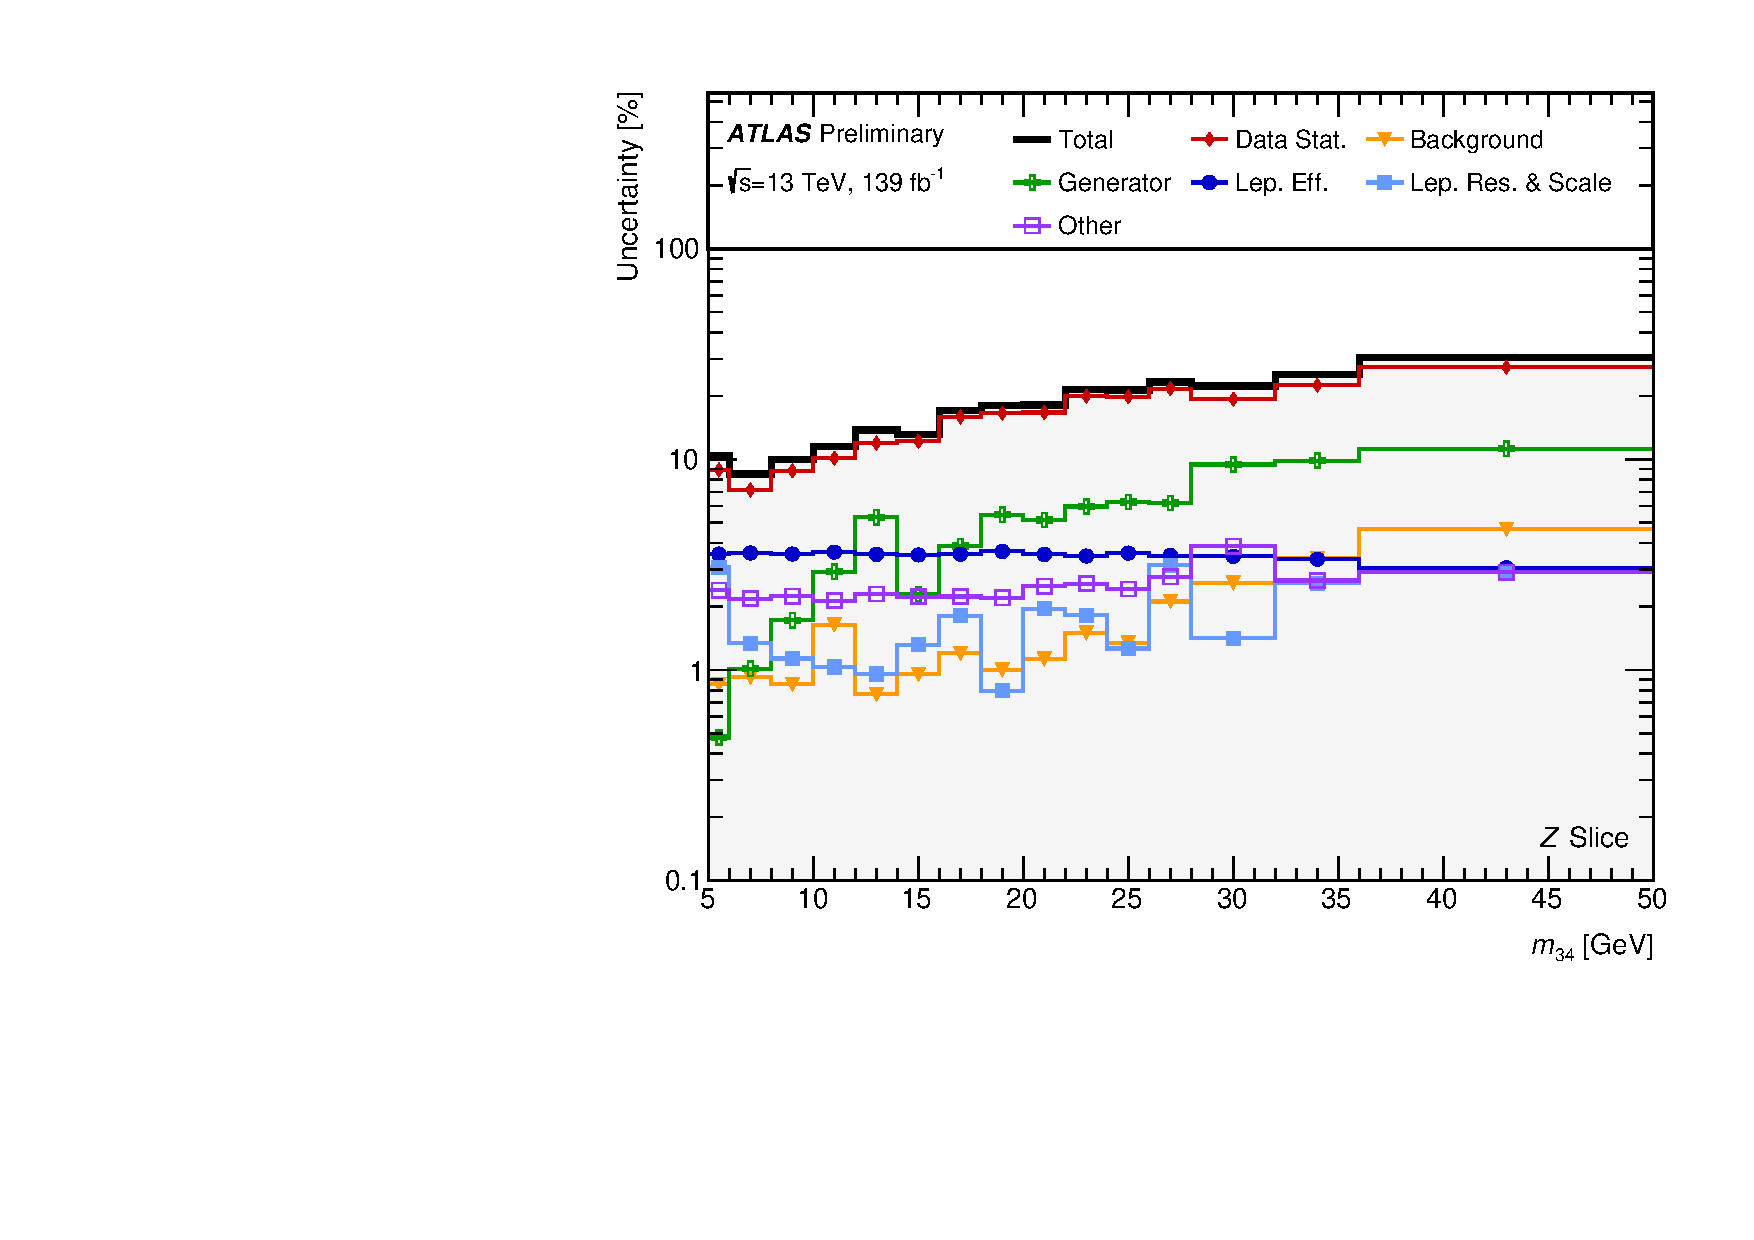
\includegraphics[width = 0.95\textwidth]{Figures/m4l/Systematics/Unfolded/UnfoldedSys_m34_vs_M4l_Stack_Paper0.pdf}\end{subfigure}
    \begin{subfigure}{.49\textwidth}\centering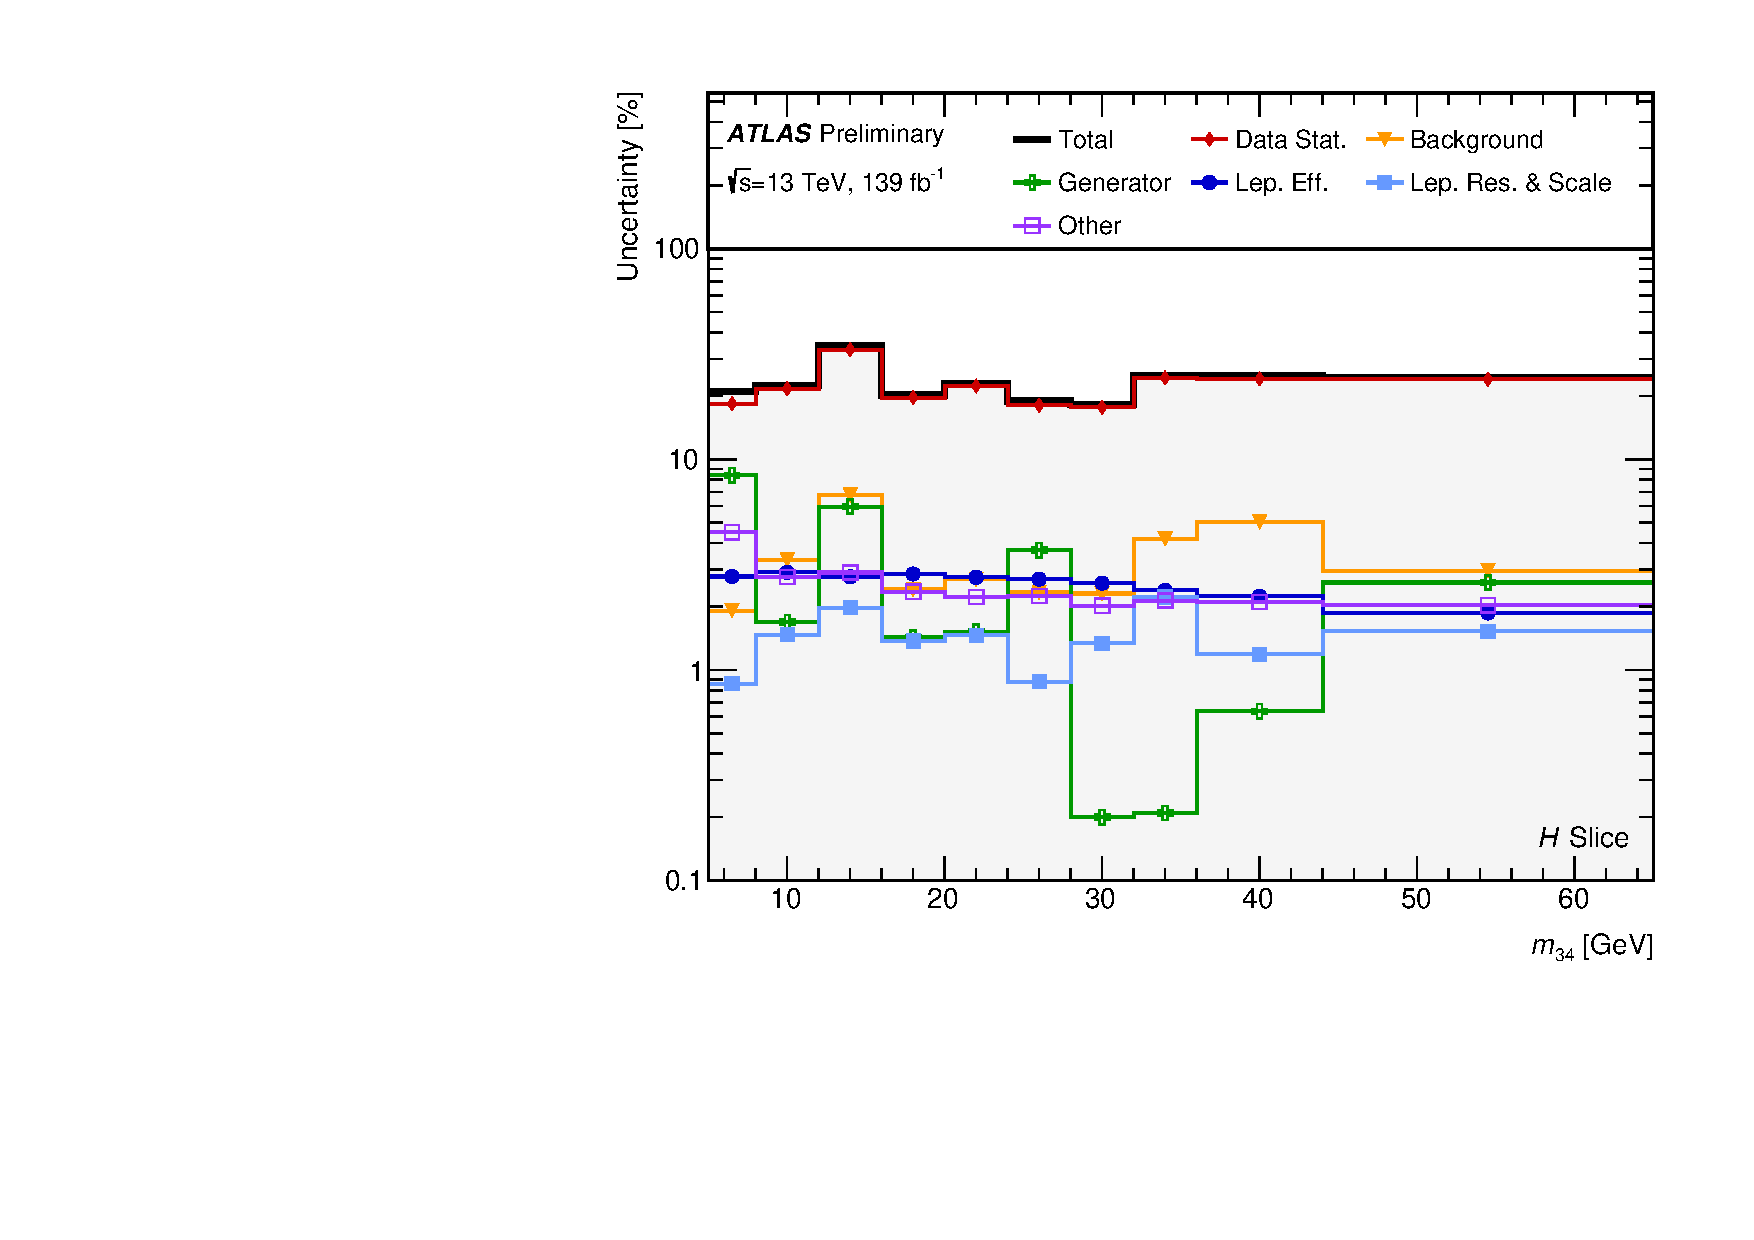
\includegraphics[width = 0.95\textwidth]{Figures/m4l/Systematics/Unfolded/UnfoldedSys_m34_vs_M4l_Stack_Paper1.pdf}\end{subfigure}
    \begin{subfigure}{.49\textwidth}\centering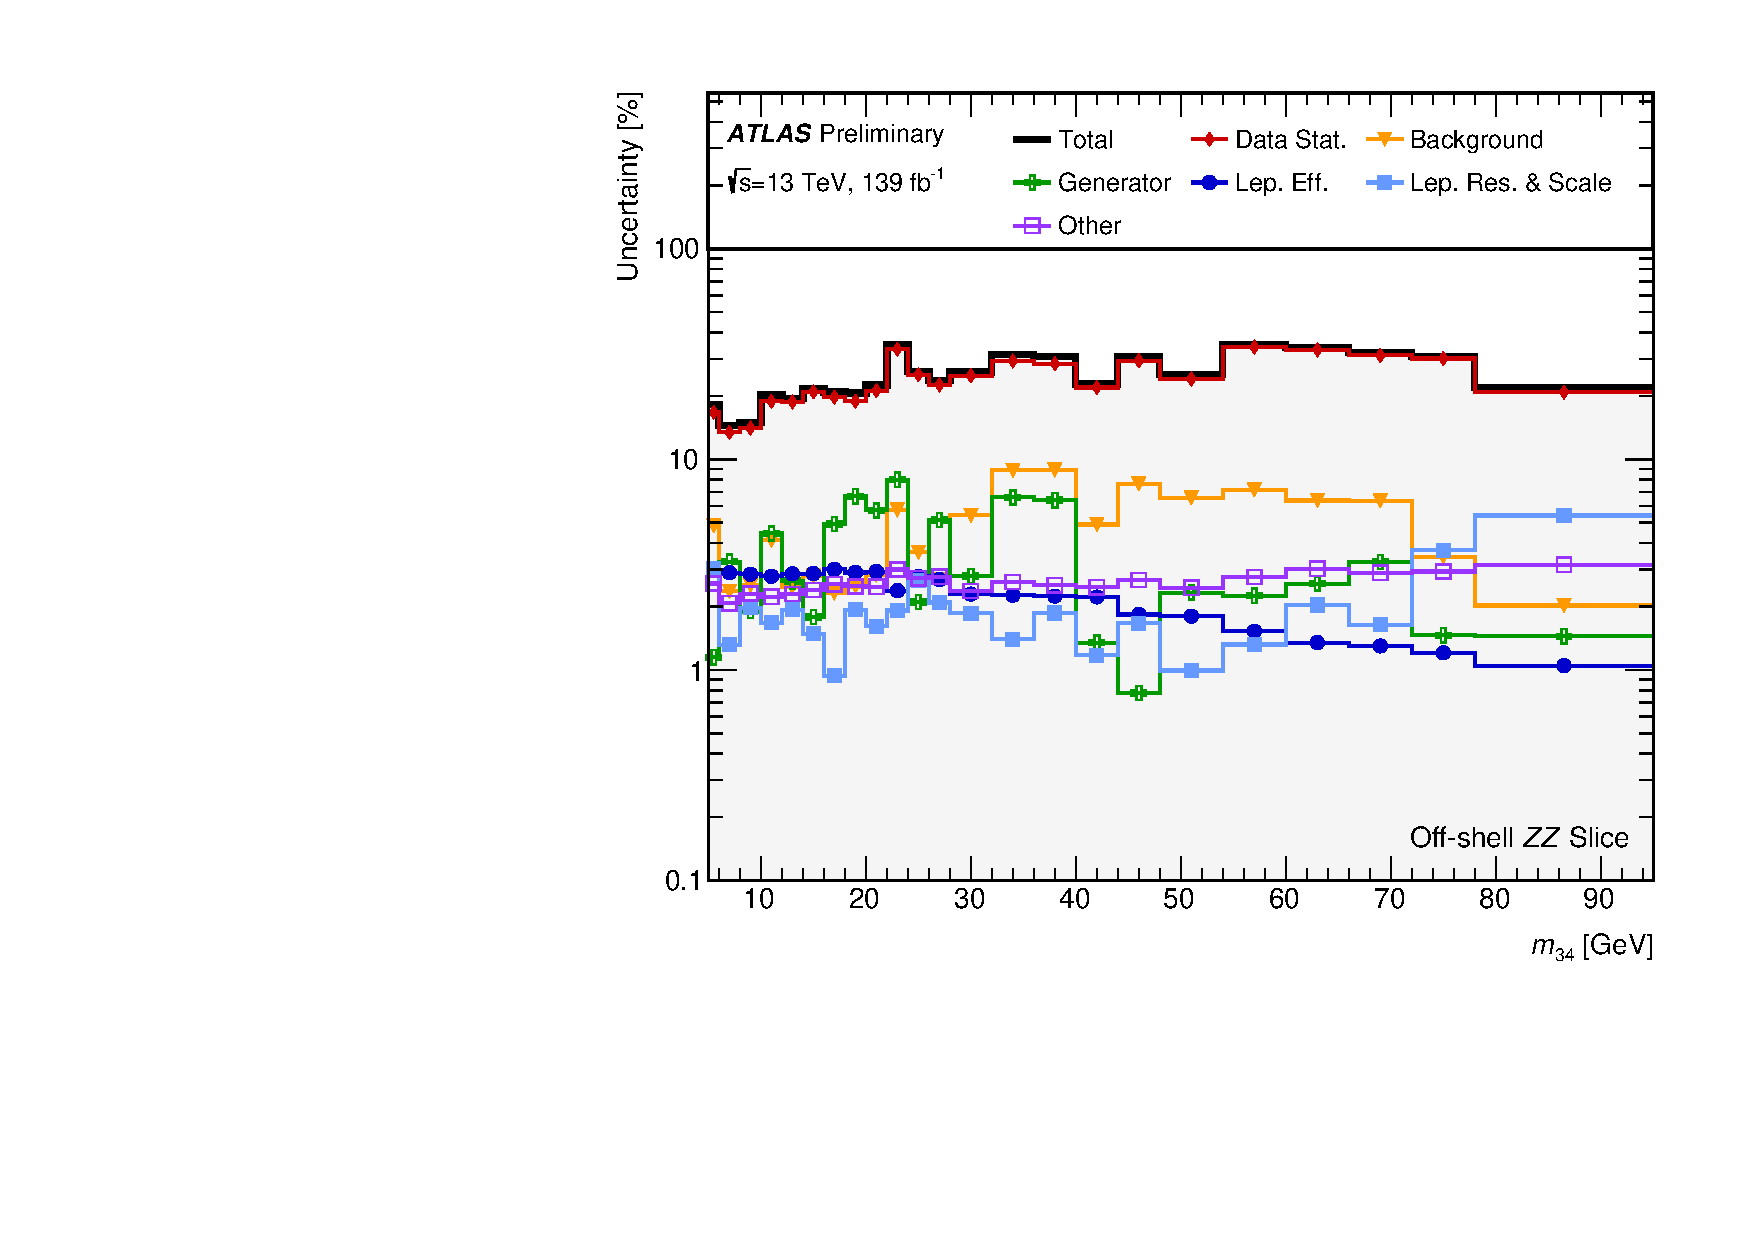
\includegraphics[width = 0.95\textwidth]{Figures/m4l/Systematics/Unfolded/UnfoldedSys_m34_vs_M4l_Stack_Paper2.pdf}\end{subfigure}
    \begin{subfigure}{.49\textwidth}\centering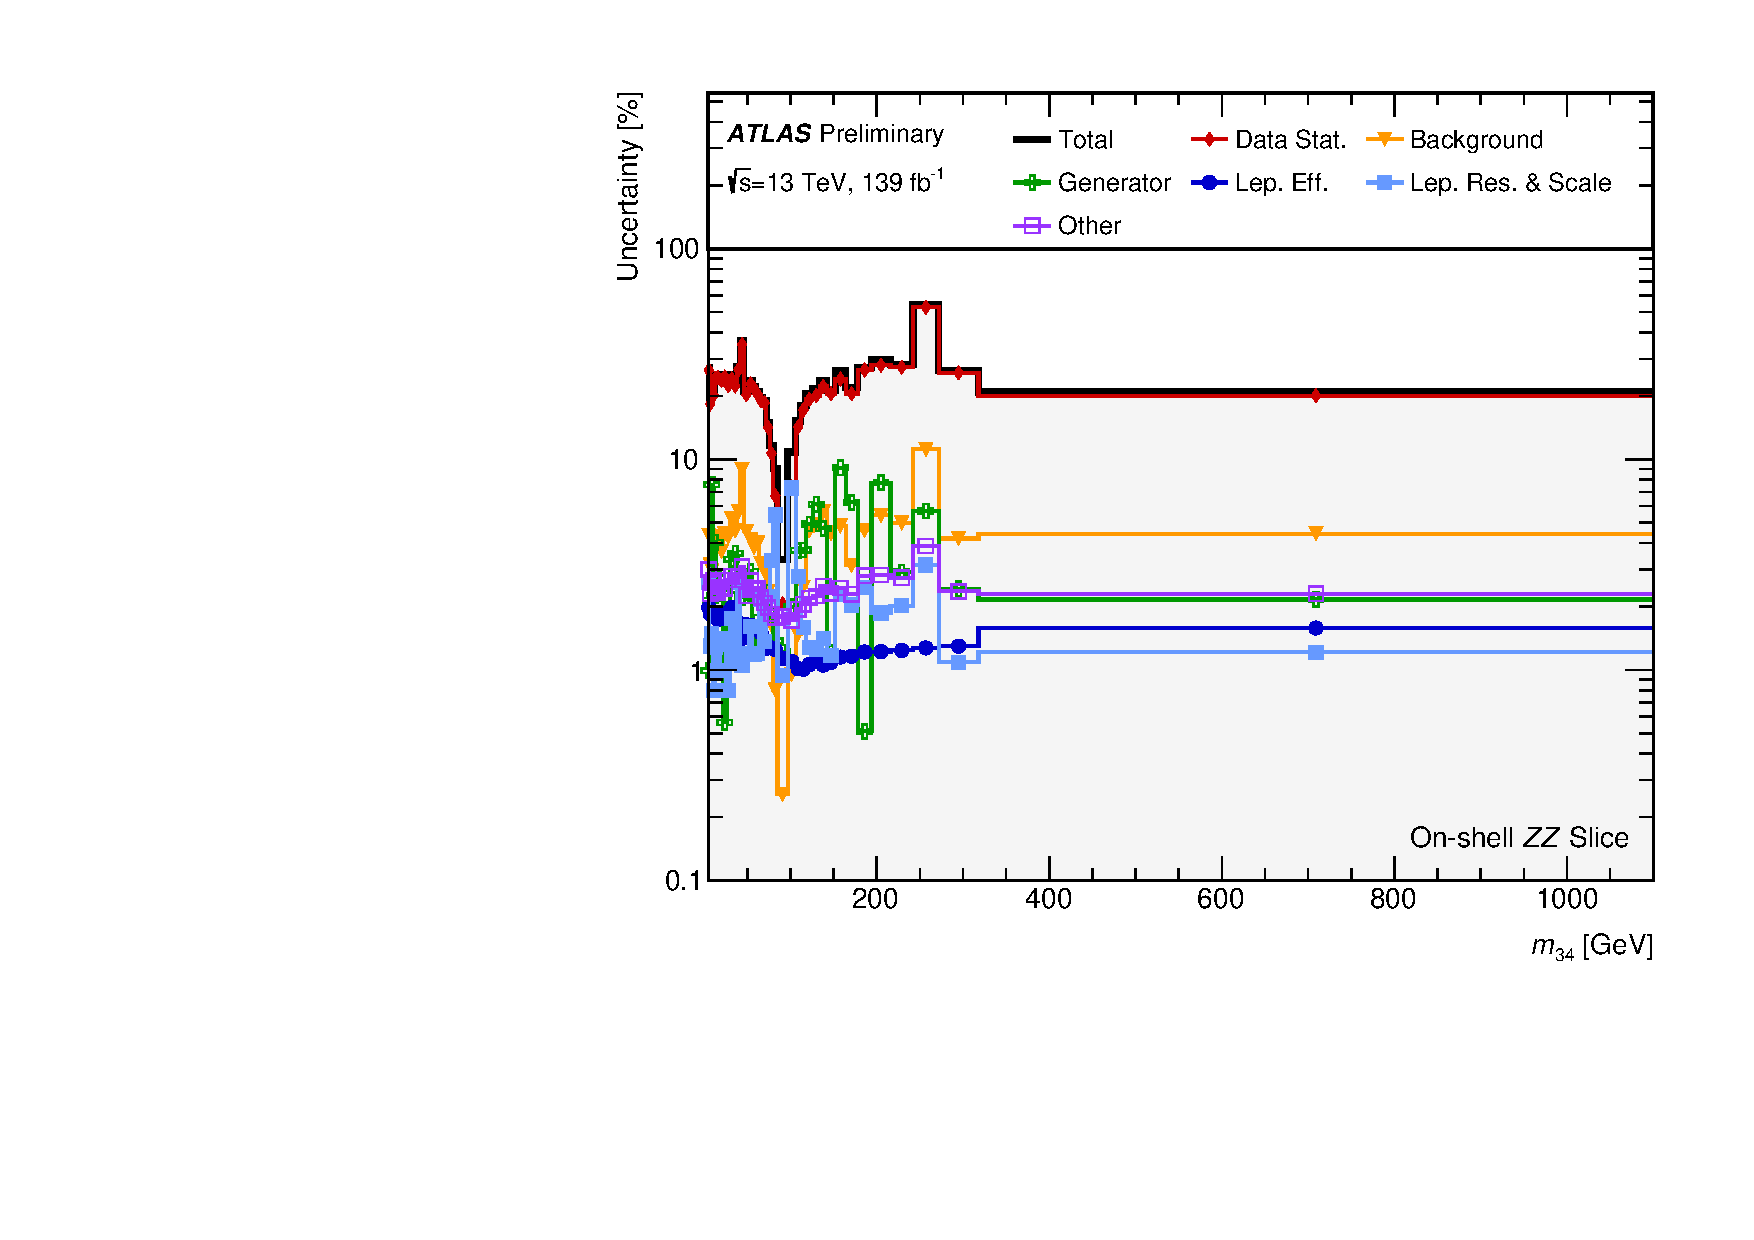
\includegraphics[width = 0.95\textwidth]{Figures/m4l/Systematics/Unfolded/UnfoldedSys_m34_vs_M4l_Stack_Paper3.pdf}\end{subfigure}
    \caption{Unfolded systematics versus $\mZTwo$, in slices of $\mFourL$.}
\end{figure}

\begin{figure}[hp]
    \centering
    \begin{subfigure}{.49\textwidth}\centering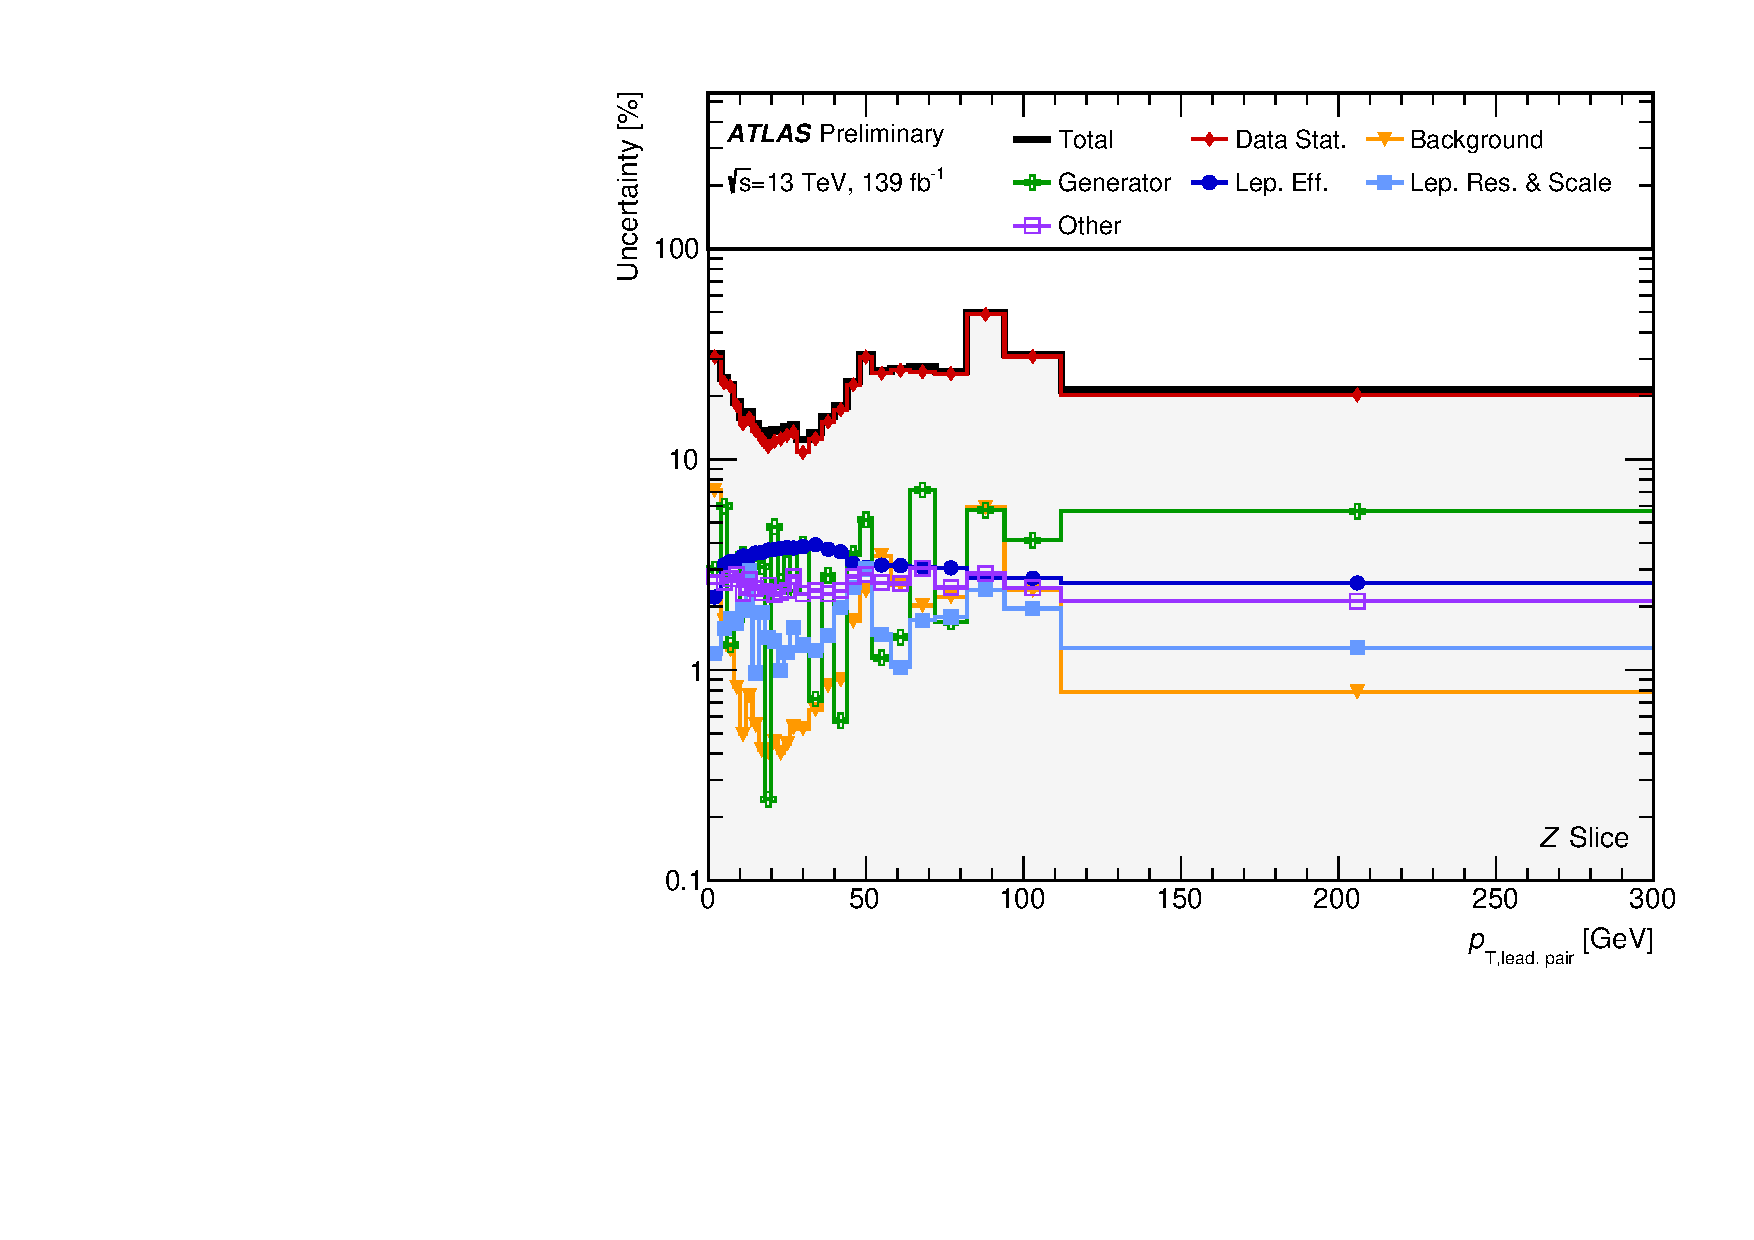
\includegraphics[width = 0.95\textwidth]{Figures/m4l/Systematics/Unfolded/UnfoldedSys_pt12_vs_M4l_Stack_Paper0.pdf}\end{subfigure}
    \begin{subfigure}{.49\textwidth}\centering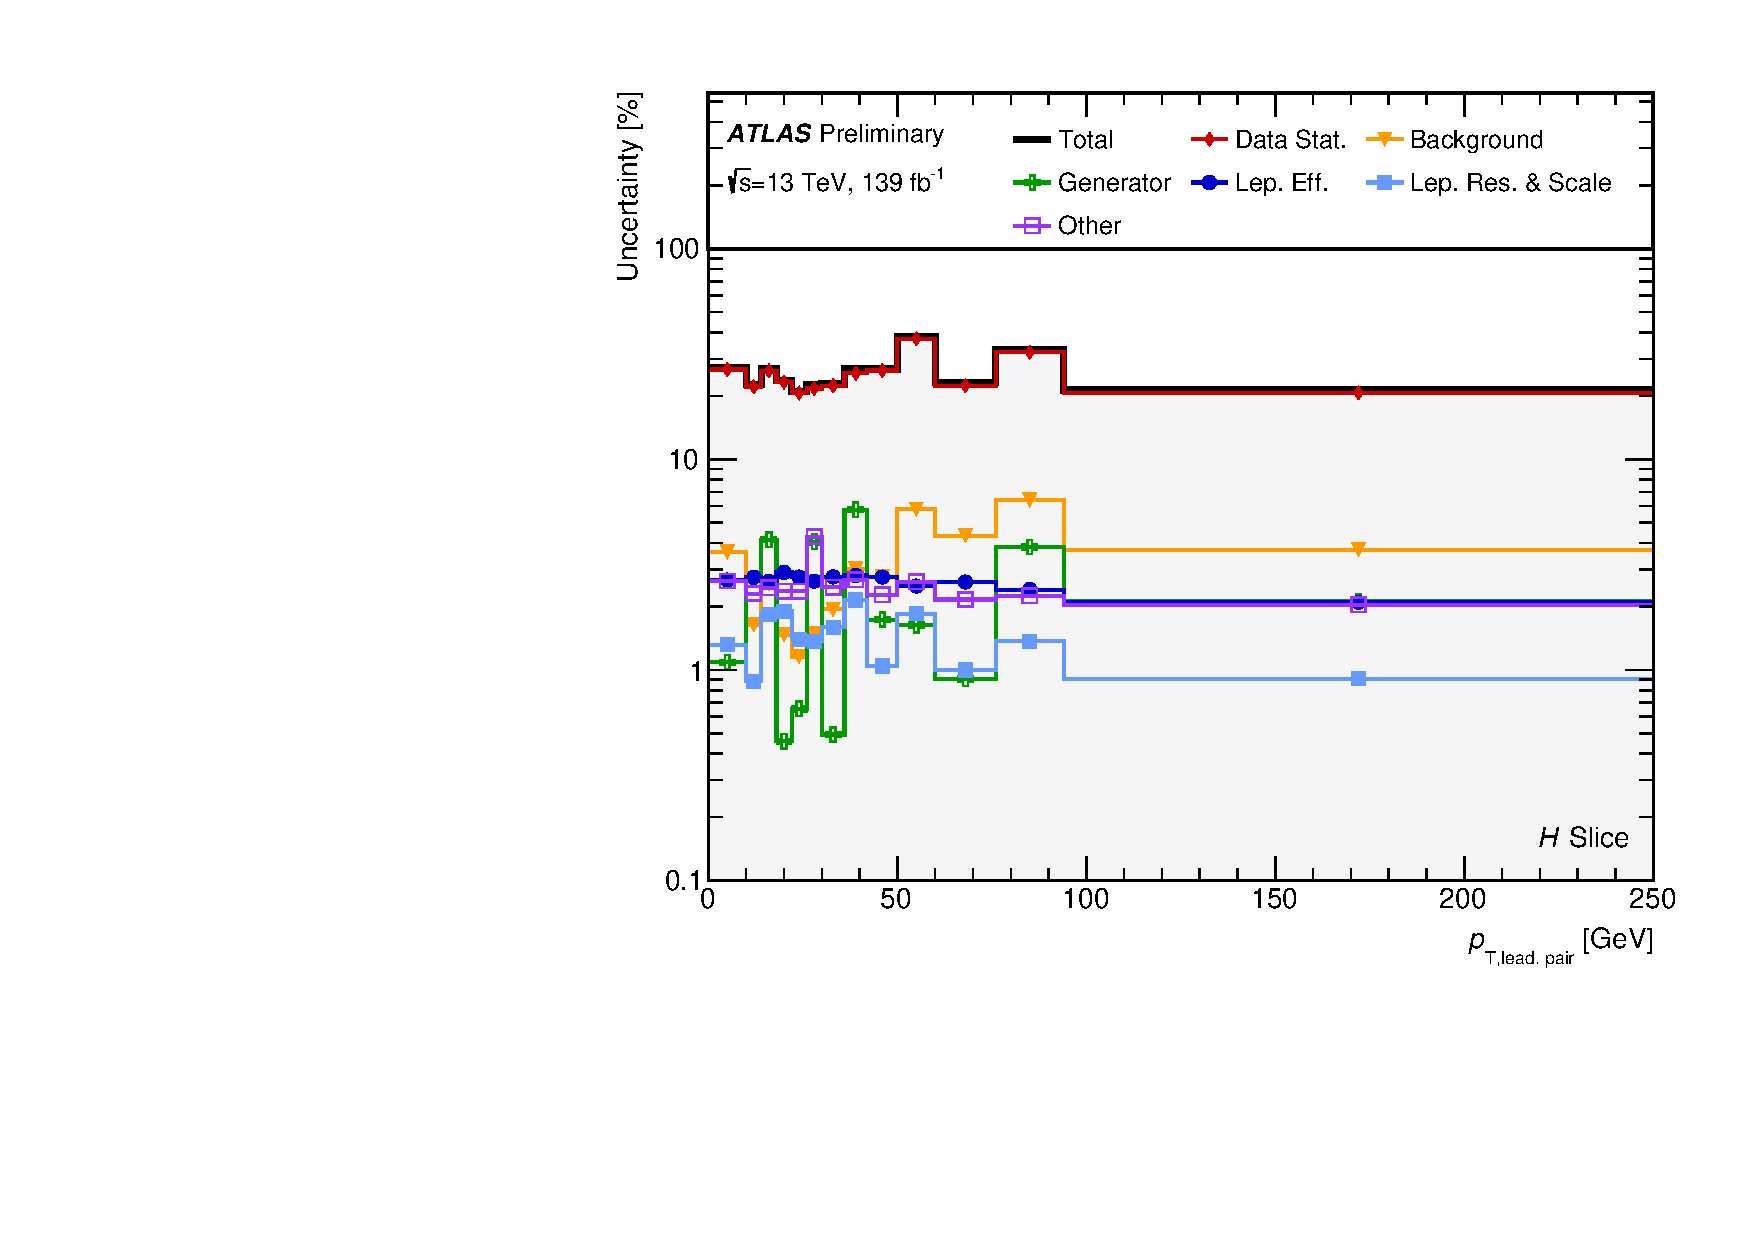
\includegraphics[width = 0.95\textwidth]{Figures/m4l/Systematics/Unfolded/UnfoldedSys_pt12_vs_M4l_Stack_Paper1.pdf}\end{subfigure}
    \begin{subfigure}{.49\textwidth}\centering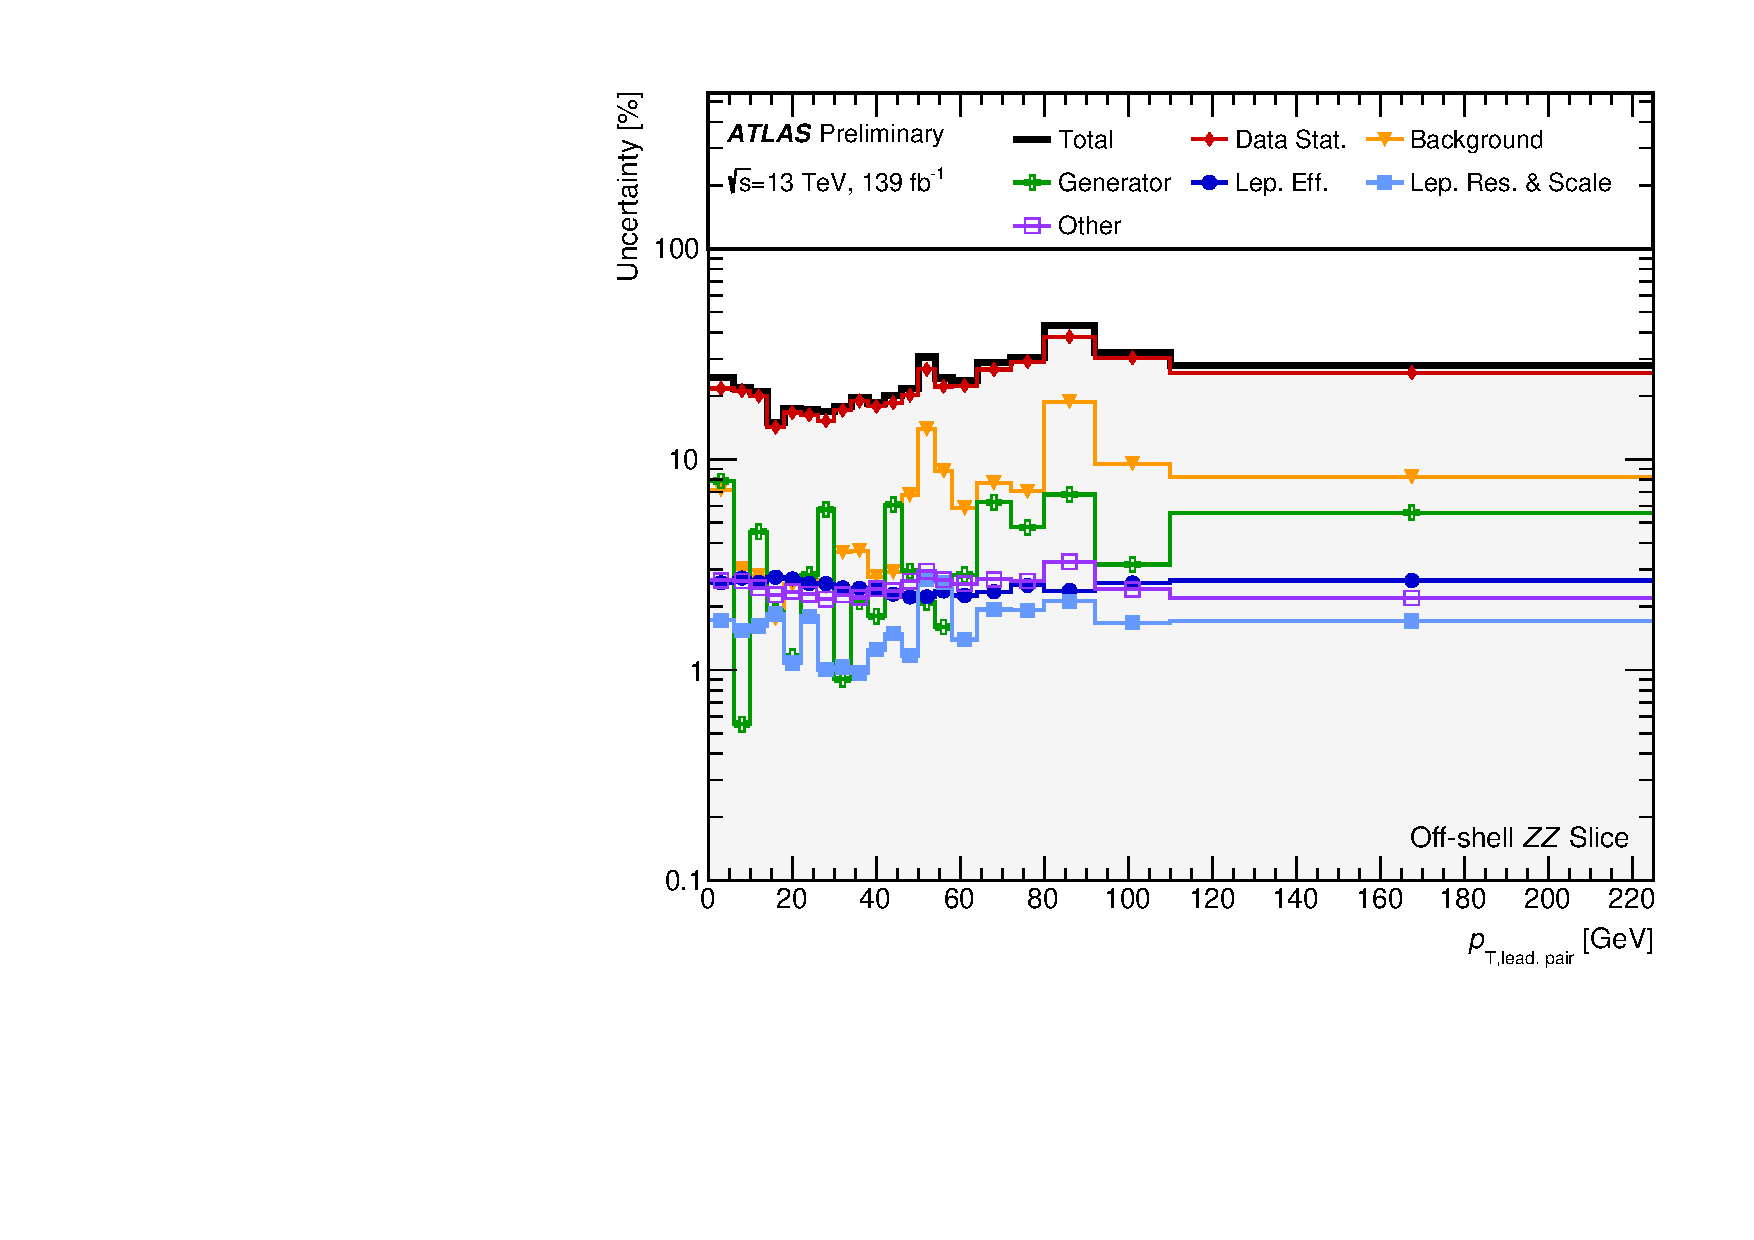
\includegraphics[width = 0.95\textwidth]{Figures/m4l/Systematics/Unfolded/UnfoldedSys_pt12_vs_M4l_Stack_Paper2.pdf}\end{subfigure}
    \begin{subfigure}{.49\textwidth}\centering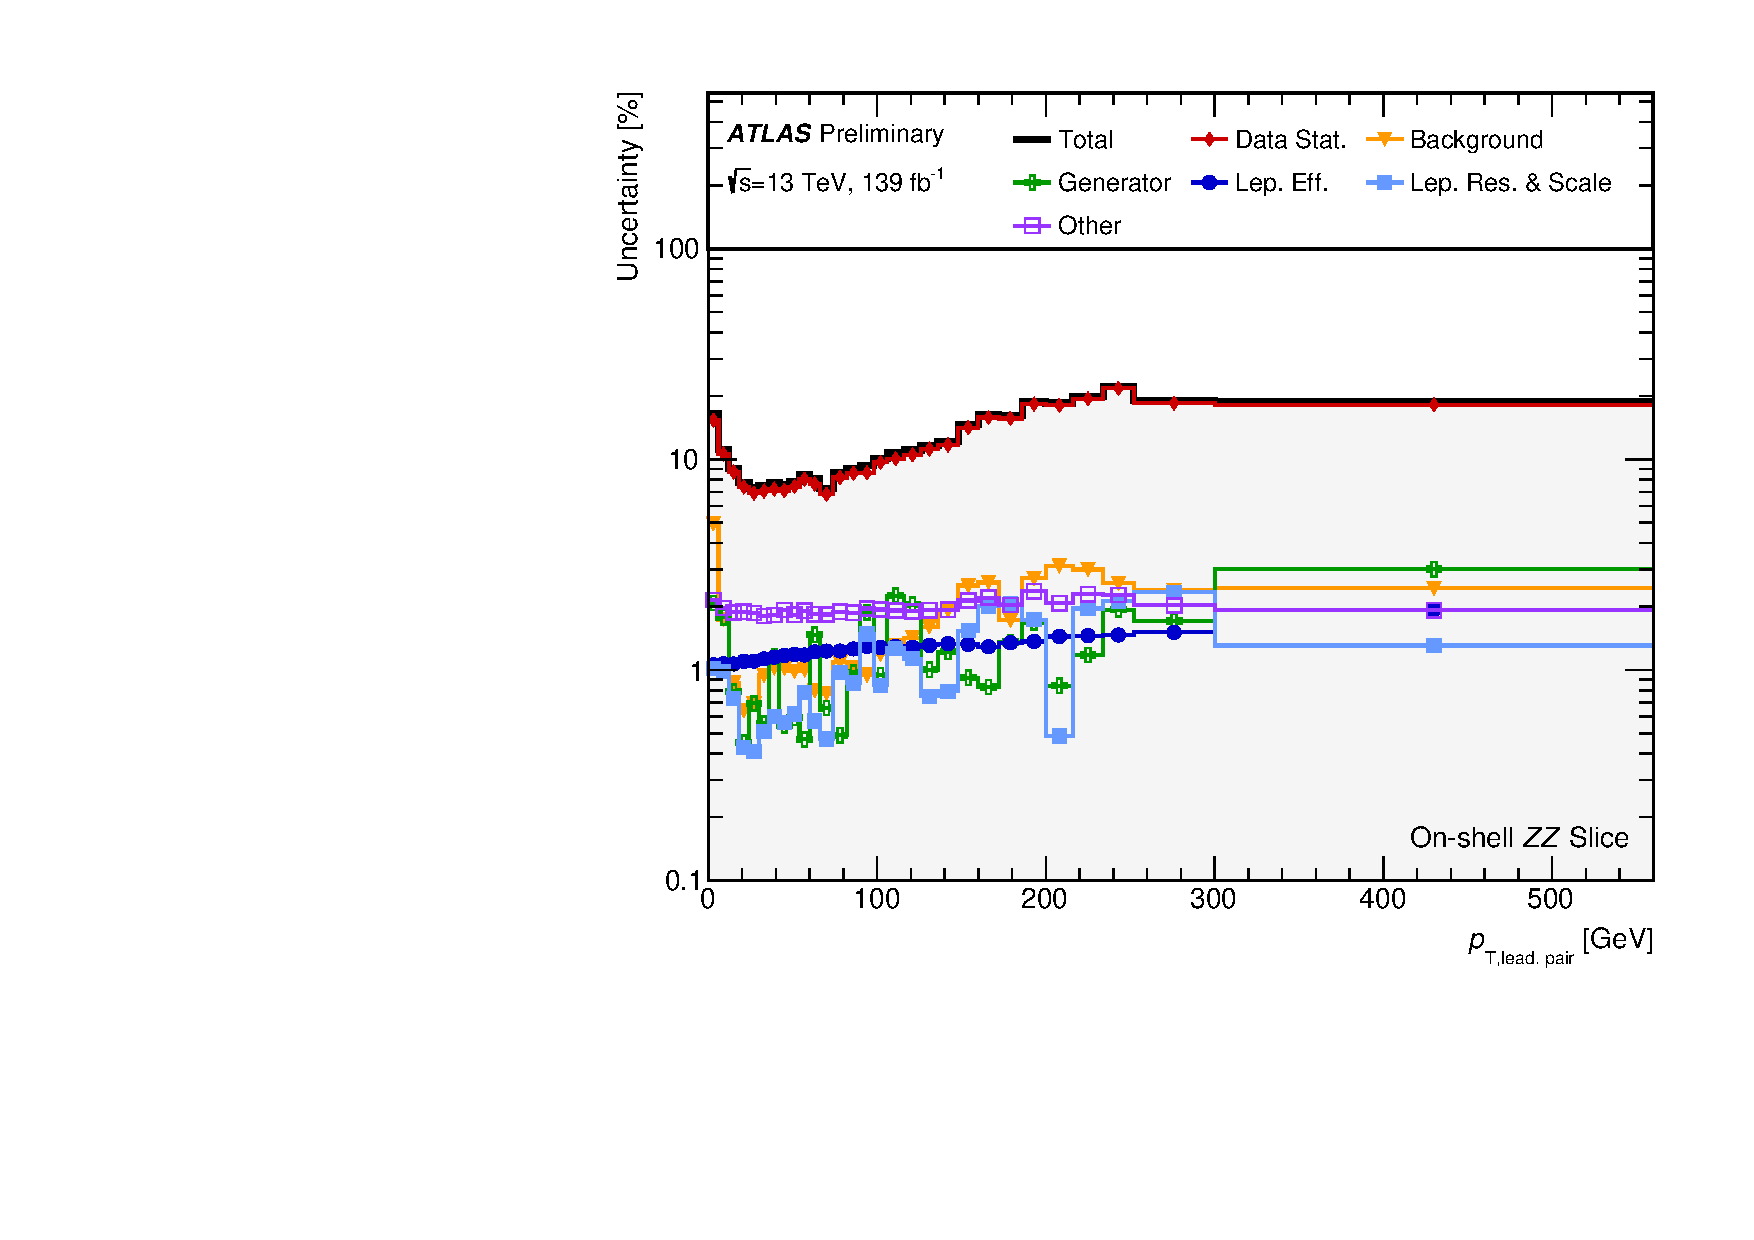
\includegraphics[width = 0.95\textwidth]{Figures/m4l/Systematics/Unfolded/UnfoldedSys_pt12_vs_M4l_Stack_Paper3.pdf}\end{subfigure}
    \caption{Unfolded systematics versus $\ptZOne$, in slices of $\mFourL$.}
\end{figure}

\begin{figure}[hp]
    \centering
    \begin{subfigure}{.49\textwidth}\centering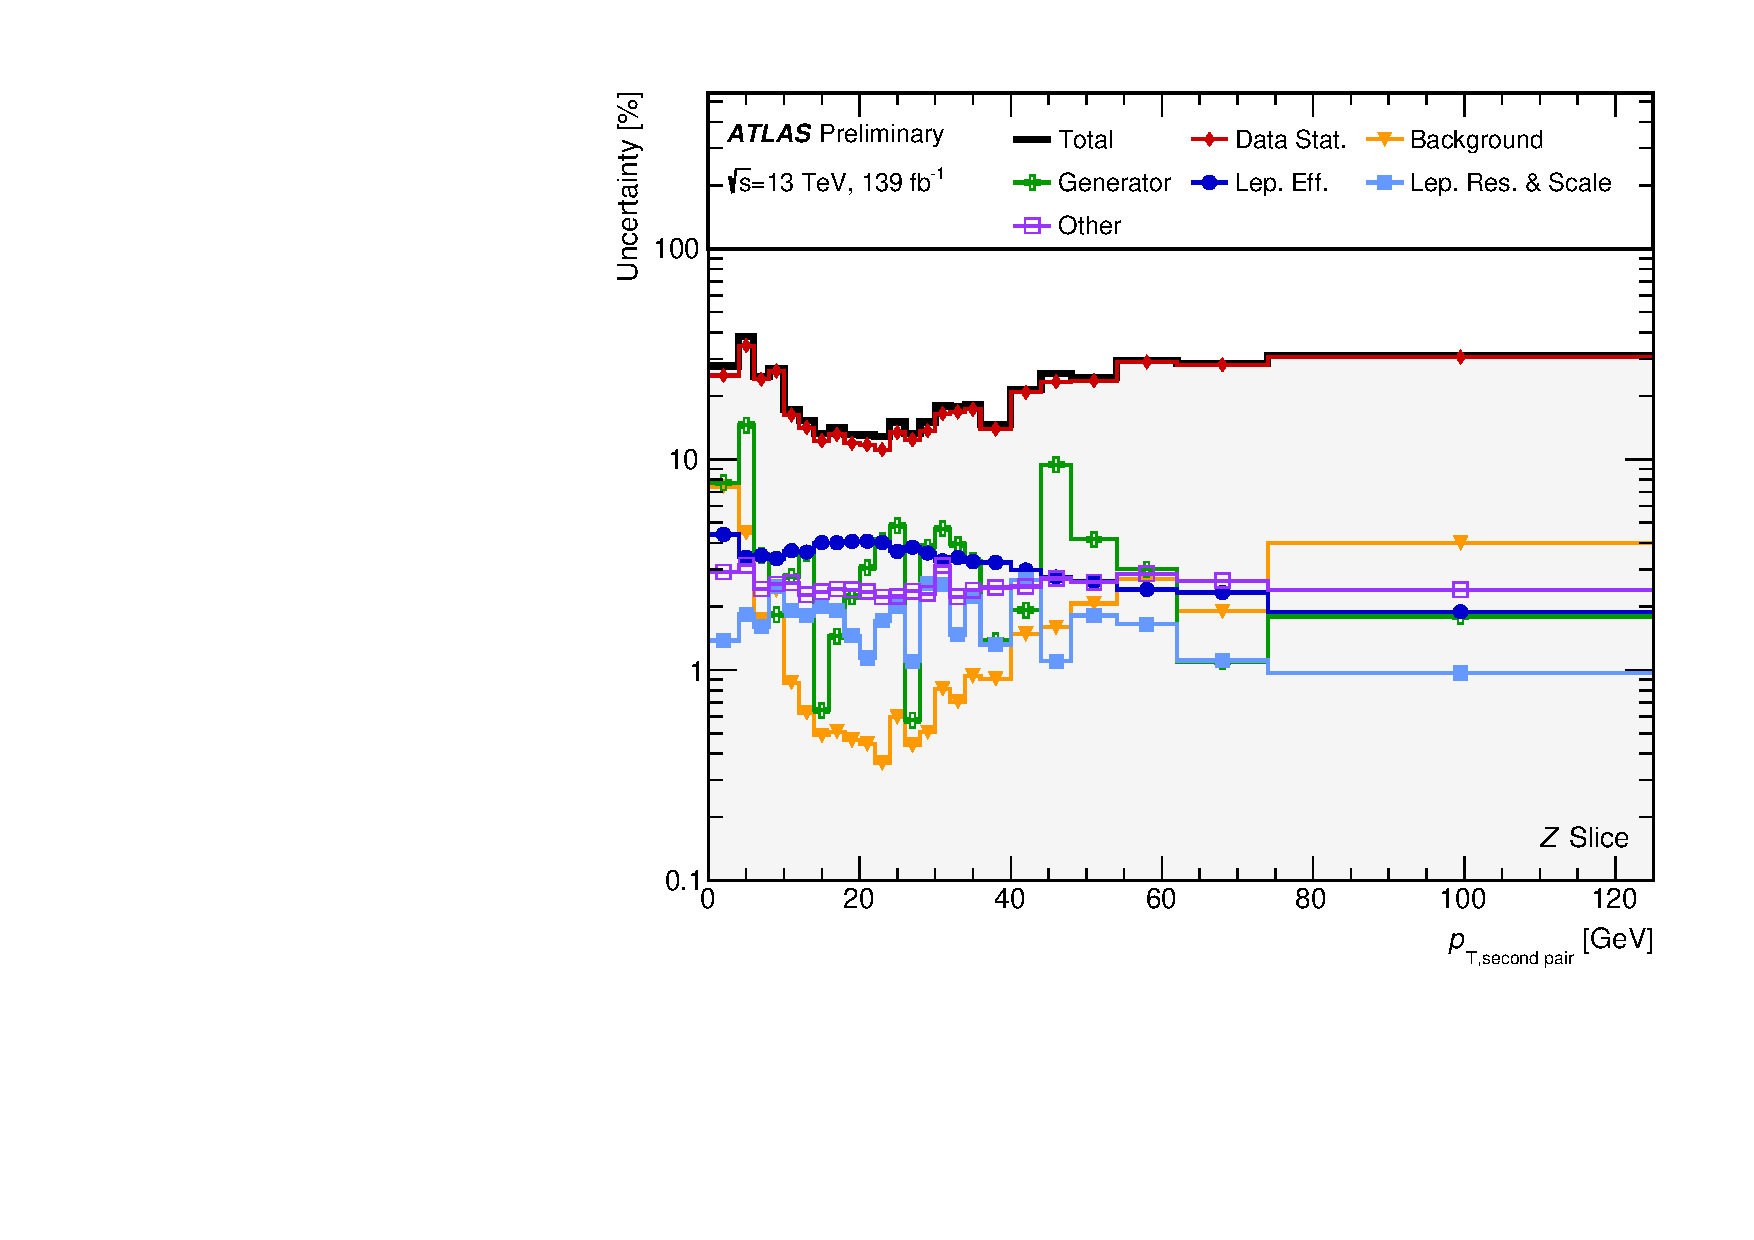
\includegraphics[width = 0.95\textwidth]{Figures/m4l/Systematics/Unfolded/UnfoldedSys_pt34_vs_M4l_Stack_Paper0.pdf}\end{subfigure}
    \begin{subfigure}{.49\textwidth}\centering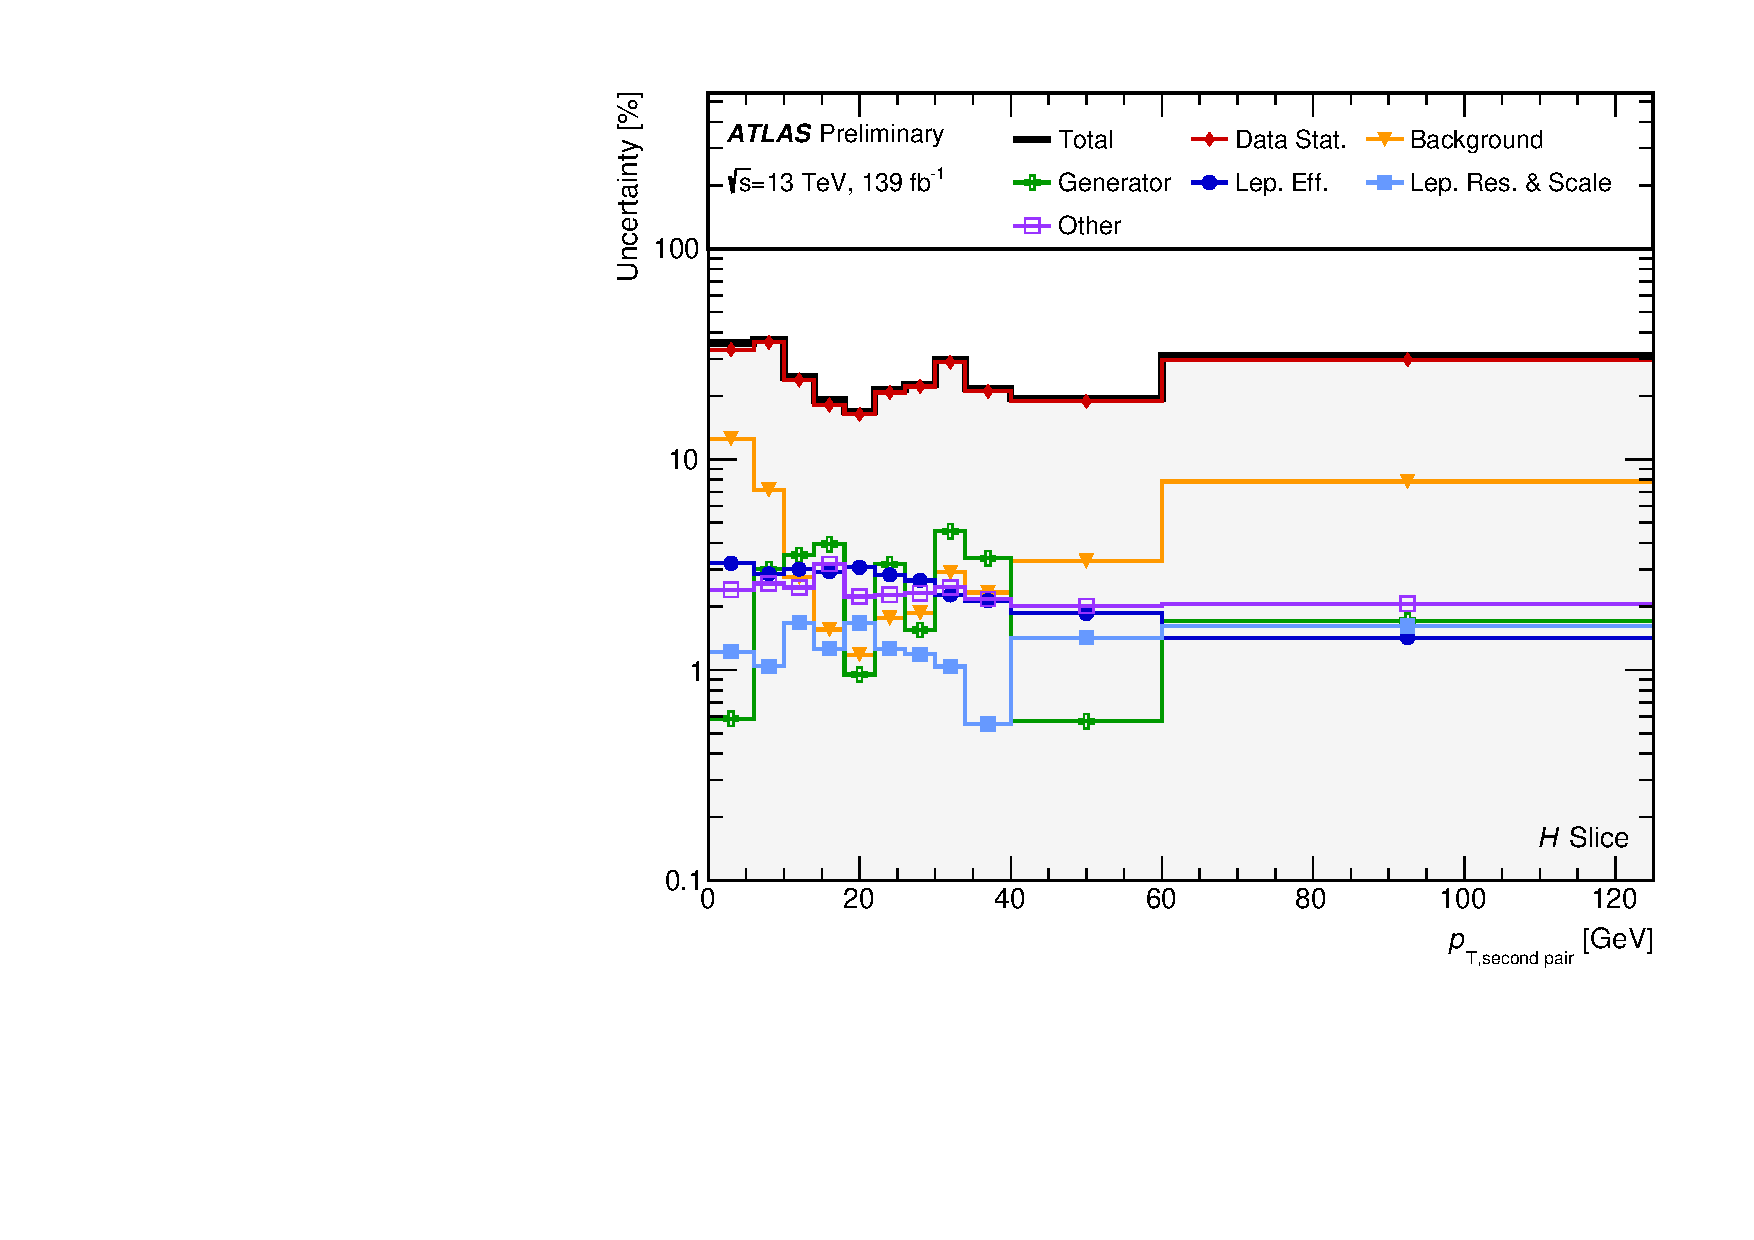
\includegraphics[width = 0.95\textwidth]{Figures/m4l/Systematics/Unfolded/UnfoldedSys_pt34_vs_M4l_Stack_Paper1.pdf}\end{subfigure}
    \begin{subfigure}{.49\textwidth}\centering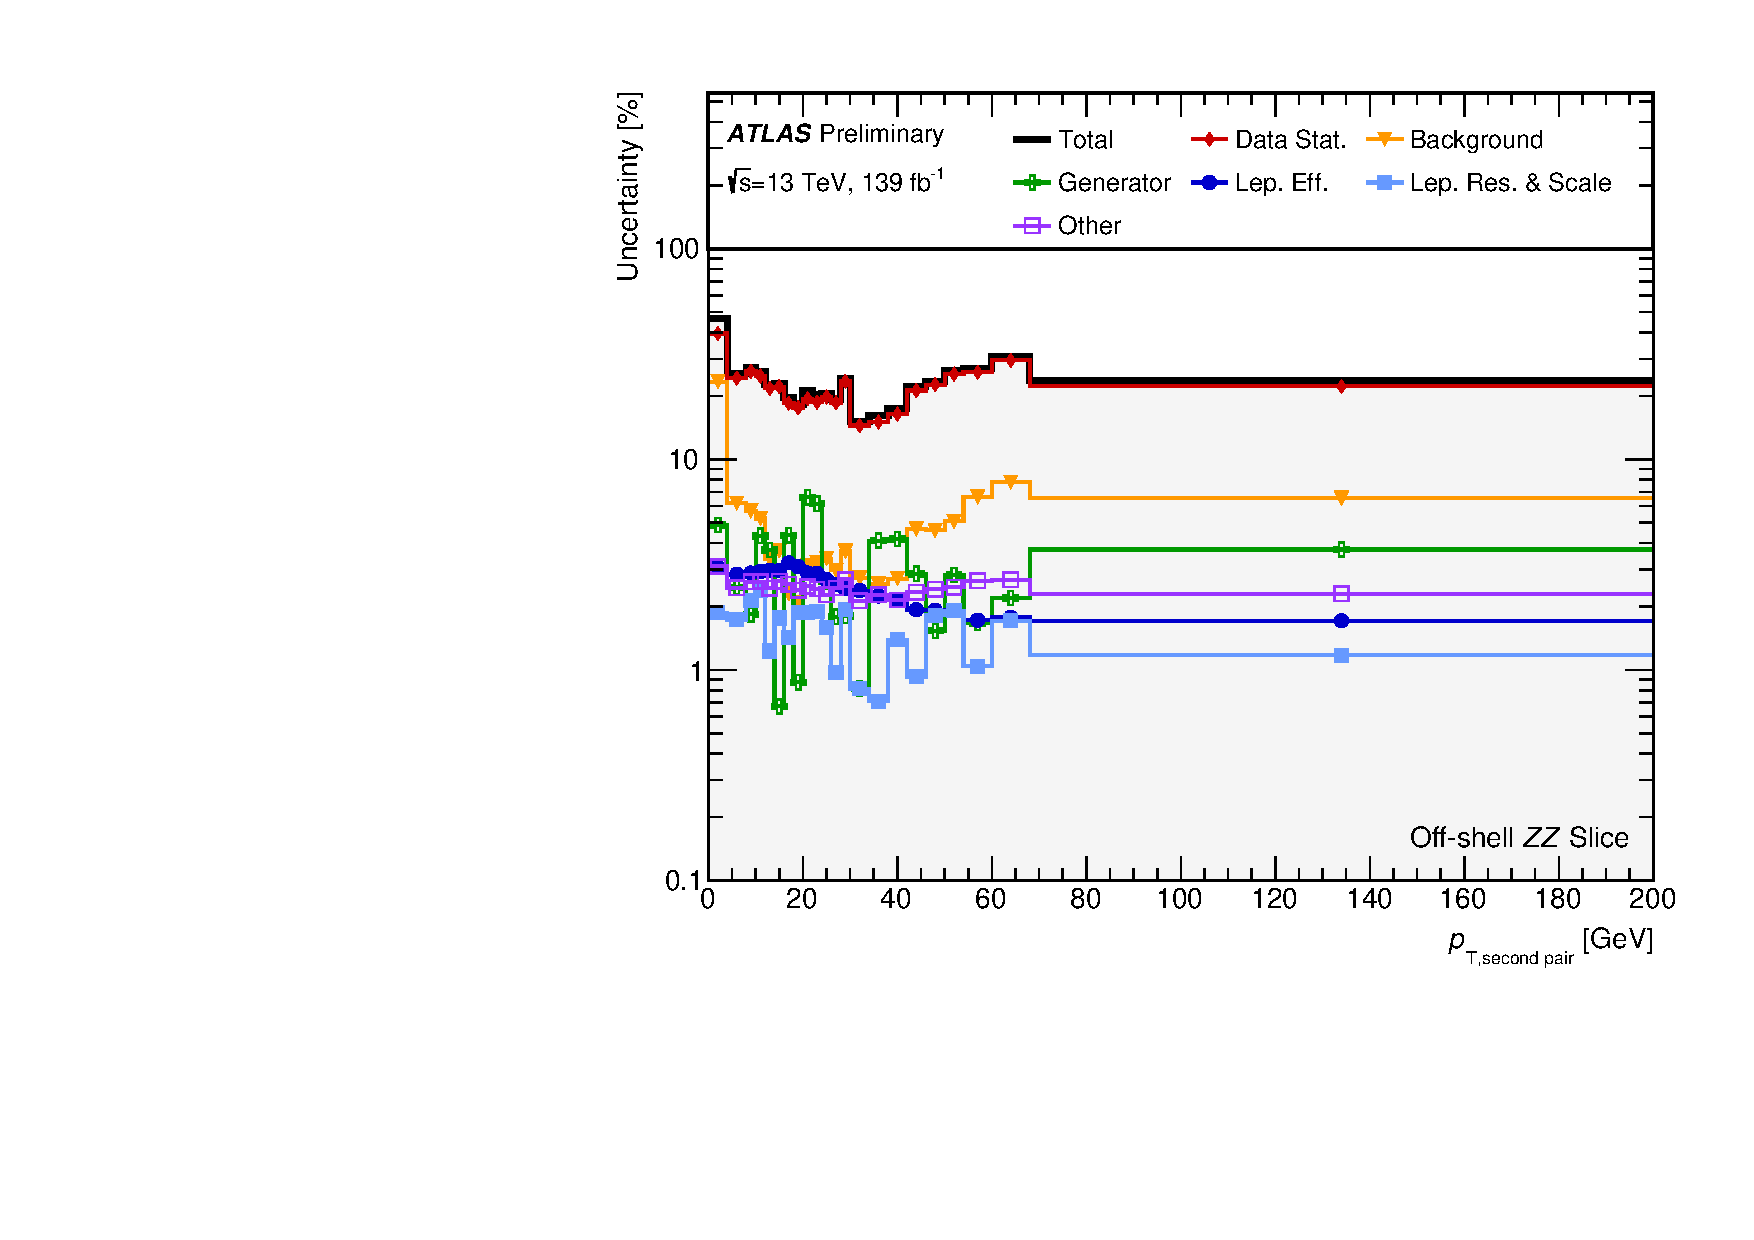
\includegraphics[width = 0.95\textwidth]{Figures/m4l/Systematics/Unfolded/UnfoldedSys_pt34_vs_M4l_Stack_Paper2.pdf}\end{subfigure}
    \begin{subfigure}{.49\textwidth}\centering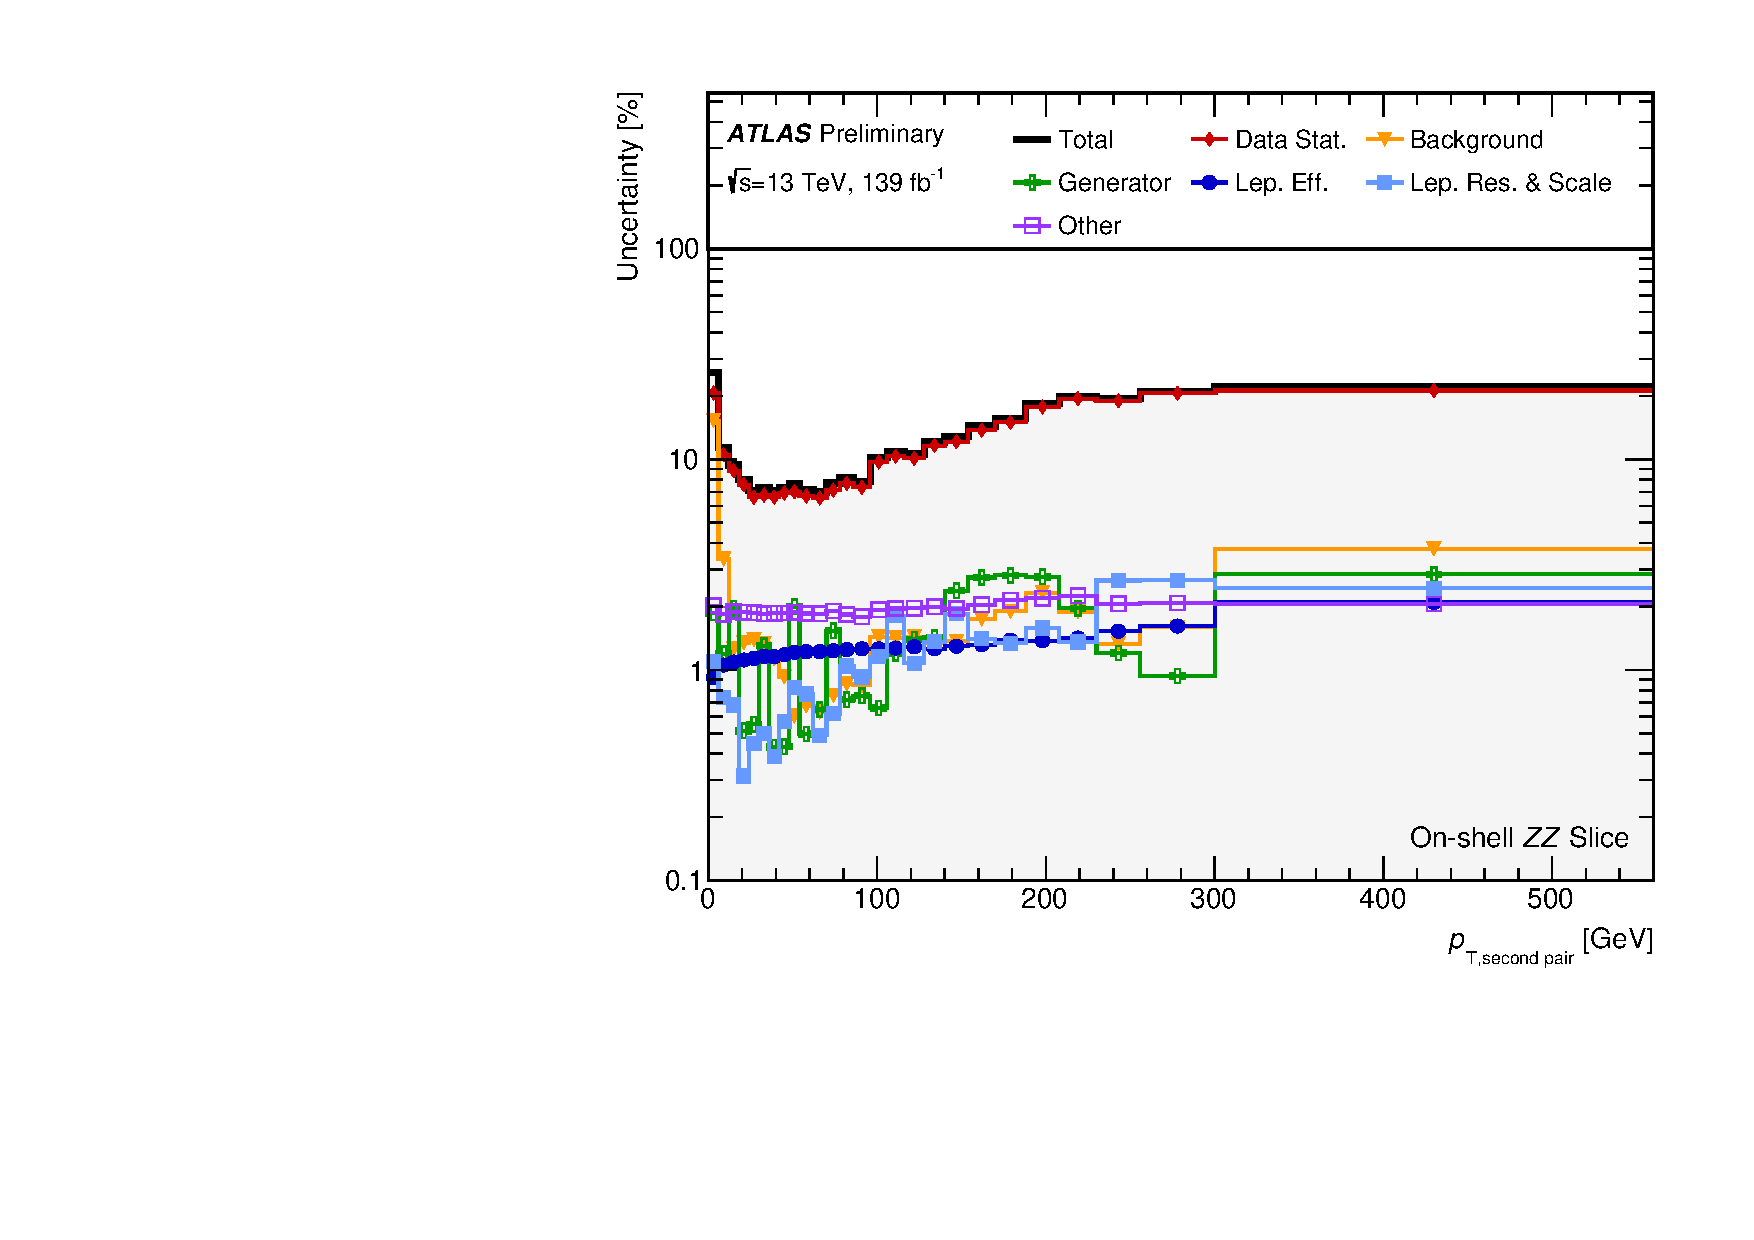
\includegraphics[width = 0.95\textwidth]{Figures/m4l/Systematics/Unfolded/UnfoldedSys_pt34_vs_M4l_Stack_Paper3.pdf}\end{subfigure}
    \caption{Unfolded systematics versus $\ptZTwo$, in slices of $\mFourL$.}
\end{figure}
